% Proposed Framework + Methodology (Updated Architecture)
% Compile with: pdflatex proposed_framework_methodology.tex
% (No results section included; this file focuses on architecture + methods.)

\documentclass[conference]{IEEEtran}

\usepackage[T1]{fontenc}
\usepackage{cite}
\usepackage{amsmath,amssymb}
\usepackage{graphicx}
\usepackage{hyperref}
\usepackage{xurl}

\usepackage{booktabs}
\usepackage{tikz}
\usetikzlibrary{arrows.meta,positioning,fit,shapes.geometric}

% Optional (for the editable Results template)
% \usepackage{booktabs}
% \usepackage{multirow}
% \usepackage{siunitx}
% \usepackage{tikz}
% \usepackage{pgfplots}
% \usepackage{pgfplotstable}
% \pgfplotsset{compat=1.18}

\hypersetup{
  hidelinks,
  pdfauthor={},
  pdftitle={Federated Agentic Defense for Zero-Day Attacks},
}

\title{Federated Agentic Defense for Zero-Day Attacks: \ \ Proposed Framework and Methodology}

\author{\IEEEauthorblockN{Author Names Omitted for Review}\n\IEEEauthorblockA{Department / University\\
Email: contact@domain}}

\begin{document}
\maketitle

\begin{abstract}
This document provides a detailed description of the proposed framework and methodology for an updated multi-agent intrusion detection and response architecture. The system combines (i) a federated unsupervised anomaly gate (Agent~1), (ii) a supervised gradient-boosted tree classifier for known attack taxonomy mapping with an explicit ``Unknown/Zero-day'' mode (Agent~2), and (iii) a retrieval-augmented large language model (LLM) action planner that generates grounded, structured mitigation steps (Agent~3). We explicitly scope federated learning claims to Agent~1 only and defer empirical evaluation results to a separate section.
\end{abstract}

\begin{IEEEkeywords}
Federated learning, intrusion detection, anomaly detection, autoencoder, XGBoost, zero-day, open set recognition, RAG, LLM, MITRE ATT\&CK, differential privacy.
\end{IEEEkeywords}

\section{Proposed Framework}
\subsection{Design Goals and Threat Model}
Modern intrusion detection systems (IDS) face two practical challenges: (i) \emph{distribution shift} and previously-unseen behaviors (``zero-day'' conditions), and (ii) \emph{data-sharing constraints} across organizations and network segments due to privacy, compliance, and operational concerns. Federated learning (FL) addresses the second challenge by allowing model training across decentralized clients without centralizing raw data \cite{mcmahan2017fedavg,kairouz2021flsurvey}. However, FL alone does not guarantee robust operational response. To close the loop, we introduce an \emph{agentic} architecture that transforms detections into actionable plans and provides interpretable context.

We assume adversaries may conduct reconnaissance, exploitation, denial-of-service, and other network-level attacks, and that labeled data for all future threats is unavailable. We also assume participating sites (clients) are \emph{honest-but-curious} by default, motivating privacy-preserving update sharing; stronger adversarial FL defenses (e.g., Byzantine robustness) are outside the scope of this methodology section \cite{blanchard2017byzantine}. 

\subsection{System Overview}
The framework consists of three cooperating agents and a coordinator:

\begin{itemize}
  \item \textbf{Agent~1 (Federated Autoencoder Anomaly Gate):} An unsupervised tabular autoencoder trained via FL across multiple clients. It produces an anomaly score from reconstruction error and serves as a fast gate to prioritize suspicious flows \cite{sakurada2014ae,chalapathy2019anomaly}.
  \item \textbf{Agent~2 (XGBoost Known-Attack Classifier + Unknown Mode):} A supervised gradient-boosted tree classifier that maps flows to a fixed attack taxonomy when confidence is sufficient; otherwise it outputs ``Unknown/Zero-day'' \cite{xgboost2016,scheirer2013openset,bendale2016openset}.
  \item \textbf{Agent~3 (RAG + LLM Action Planner):} A retrieval-augmented generation module that queries a threat-intelligence knowledge base (e.g., ATT\&CK techniques, CVE summaries, playbooks) and uses an LLM to output structured mitigation steps grounded in retrieved evidence \cite{lewis2020rag,attck,cve,nist80061}.
  \item \textbf{Integration Coordinator:} Orchestrates the inference-time pipeline and assembles a unified semantic threat report for analyst consumption.
\end{itemize}

\subsection{Inference-Time Data Flow}
Let $x \in \mathbb{R}^d$ denote a single preprocessed network-flow feature vector.

\subsubsection{Stage~1: Agent~1 anomaly scoring}
Agent~1 computes a reconstruction $\hat{x}$ and anomaly score $s(x)$:
\begin{equation}
  s(x) = \frac{1}{d}\lVert x - \hat{x} \rVert_2^2.
  \label{eq:recon_error}
\end{equation}
A threshold $\tau$ converts $s(x)$ to a binary anomaly decision. If $s(x) > \tau$, the sample is flagged as anomalous and forwarded with high priority.

\subsubsection{Stage~2: Agent~2 taxonomy classification with ``Unknown'' mode}
Agent~2 produces class probabilities $p(c\mid x)$ over a known label set $\mathcal{C}$ (e.g., standard IDS categories). The predicted label is:
\begin{equation}
  \hat{c} = \arg\max_{c \in \mathcal{C}} p(c\mid x).
\end{equation}
To represent novelty or ambiguity, we apply an open-set style decision rule:
\begin{equation}
  y(x) =
  \begin{cases}
    \hat{c}, & \max_{c \in \mathcal{C}} p(c\mid x) \ge \gamma \\
    \text{Unknown/Zero-day}, & \text{otherwise,}
  \end{cases}
  \label{eq:unknown_rule}
\end{equation}
where $\gamma$ is a confidence threshold. This prevents forced misclassification when evidence is weak and provides an explicit operational trigger for deeper analysis \cite{scheirer2013openset,bendale2016openset}.

\subsubsection{Stage~3: Agent~3 retrieval and action planning (RAG)}
Agent~3 constructs a query from upstream signals (anomaly score, predicted category, confidence, optional mapped technique hints). It retrieves top-$k$ relevant passages from a vector index and prompts an LLM to produce structured mitigation actions grounded in the retrieved evidence \cite{lewis2020rag}.

\subsubsection{Coordinator output}
The coordinator returns a semantic report containing: anomaly decision and score; classification (or Unknown) and confidence; retrieved references (CVE/ATT\&CK/KB snippets); and an action plan with prioritized steps.

\subsection{Federated Scope Claim (Explicit)}
This work \textbf{claims federated learning for Agent~1 only}. FedAvg-style aggregation applies directly to neural network parameters \cite{mcmahan2017fedavg}. In contrast, direct weight averaging for tree ensembles is non-trivial; federated boosting requires specialized procedures beyond FedAvg \cite{kairouz2021flsurvey}. Accordingly, Agent~2 is treated as centrally trained or locally trained per-site within this methodology.

\section{System Architecture of the Proposed Framework}
\label{sec:system_architecture}

This section summarizes the end-to-end architecture and how components interact at runtime and during federated training. We focus on \emph{connectivity, responsibilities, and control flow} rather than the internal details of each agent (which are provided in the Methodology section).

\subsection{Top-Level Components}
The proposed system comprises five logical components:
\begin{itemize}
  \item \textbf{Data plane (network flows):} Raw traffic is summarized into flow records (e.g., UNSW-NB15-style features) and preprocessed into a fixed-dimensional vector $x \in \mathbb{R}^d$.
  \item \textbf{Agent~1 (Federated anomaly gate):} A lightweight unsupervised gate that filters benign traffic early and forwards suspicious flows downstream. This is the \emph{only} component trained via FL in our framework \cite{mcmahan2017fedavg}.
  \item \textbf{Agent~2 (Known-attack classifier + Unknown mode):} A fast supervised classifier that labels known attack families when confident and emits \emph{Unknown/Zero-day} otherwise to prevent forced misclassification.
  \item \textbf{Agent~3 (RAG+LLM action planner):} A retrieval-augmented planner that produces a grounded analyst-facing report and recommended mitigations using external threat intelligence \cite{lewis2020rag,attck,cve,nist80061}.
  \item \textbf{Coordinator (orchestrator):} Executes the staged pipeline, applies routing policies, and aggregates outputs into a single incident record.
\end{itemize}

\subsection{Connectivity and Execution Semantics}
The runtime pipeline is intentionally \emph{hierarchical}: most flows terminate at Agent~1 (benign), fewer reach Agent~2 (suspicious), and only the lowest-confidence / unknown cases invoke Agent~3 (expensive reasoning). This selective offloading reduces LLM calls and yields a practical ``defense-in-depth'' control flow.

\textbf{Routing policy.} A flow $x$ is processed as follows:
\begin{enumerate}
  \item Agent~1 produces an anomaly score $s(x)$ and gate decision.
  \item If anomalous, Agent~2 outputs $(\hat{c}, c(x))$ where $\hat{c}$ is the predicted class and $c(x)$ is confidence; if $c(x)$ is low, it returns \emph{Unknown/Zero-day}.
  \item The coordinator invokes Agent~3 when (i) Agent~2 returns Unknown, or (ii) confidence is below a configured threshold, or (iii) the incident requires contextual enrichment.
\end{enumerate}

\subsection{Federated Learning Placement and Purpose}
Federated learning is introduced to address cross-site data-sharing constraints while improving generalization of the \emph{anomaly gate}. Each client trains Agent~1 locally on its private, potentially non-IID traffic, and a server aggregates updates into a global model using FedAvg \cite{mcmahan2017fedavg,kairouz2021flsurvey}. The resulting global anomaly gate reduces site-specific blind spots while avoiding raw data pooling.

\subsection{Fed--RAG Bridge: Why It Exists and What It Does}
The \emph{Fed--RAG bridge} connects learning dynamics in Agent~1 to the knowledge-grounded explanation and action layer in Agent~3. Its purpose is to ensure that when the federated anomaly detector evolves (across rounds, clients, and non-IID conditions), the system:
\begin{itemize}
  \item maintains consistent operator-facing explanations for ``why this is anomalous,'' and
  \item refreshes retrieval context and suggested mitigations when the anomaly profile indicates drift or novelty.
\end{itemize}

At a high level, the bridge monitors federated-round metadata (e.g., reconstruction-error distribution shifts, threshold movement, and client-specific score statistics). When a drift signal exceeds a significance threshold, the bridge triggers Agent~3 to regenerate or update the evidence pack and action plan for representative flagged samples. This introduces an explicit mechanism for \emph{keeping the explanation layer aligned} with the evolving detector, while preserving the FL constraint that raw traffic is not centralized.

\begin{figure*}[t]
\centering
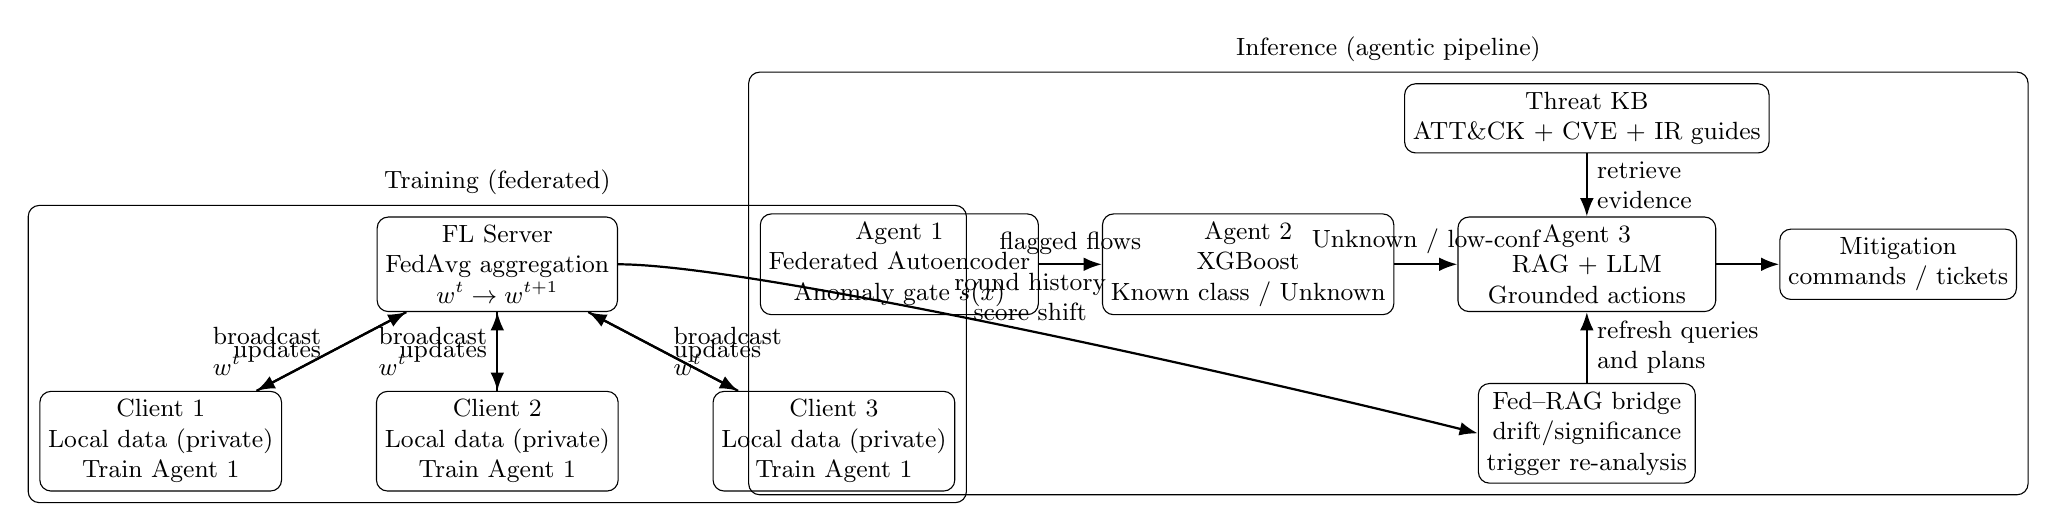
\begin{tikzpicture}[
  font=\small,
  node distance=7mm and 9mm,
  box/.style={draw, rounded corners, align=center, minimum height=7mm, inner sep=3pt},
  bigbox/.style={box, minimum width=0.27\textwidth},
  sbox/.style={box, minimum width=0.19\textwidth},
  arr/.style={-Latex, thick}
]

% --- Training side (FL) ---
\node[box, minimum width=0.23\textwidth] (flsrv) {FL Server\\FedAvg aggregation\\$w^{t}\rightarrow w^{t+1}$};
\node[sbox, below left=10mm and 12mm of flsrv] (c1) {Client 1\\Local data (private)\\Train Agent 1};
\node[sbox, below=10mm of flsrv] (c2) {Client 2\\Local data (private)\\Train Agent 1};
\node[sbox, below right=10mm and 12mm of flsrv] (c3) {Client 3\\Local data (private)\\Train Agent 1};

\draw[arr] (flsrv) -- node[left, align=left] {broadcast\\$w^t$} (c1);
\draw[arr] (flsrv) -- node[left, align=left] {broadcast\\$w^t$} (c2);
\draw[arr] (flsrv) -- node[right, align=left] {broadcast\\$w^t$} (c3);

\draw[arr] (c1) -- node[left, align=left] {updates} (flsrv);
\draw[arr] (c2) -- node[left, align=left] {updates} (flsrv);
\draw[arr] (c3) -- node[right, align=left] {updates} (flsrv);

% --- Inference side (pipeline) ---
\node[bigbox, right=18mm of flsrv] (a1) {Agent 1\\Federated Autoencoder\\Anomaly gate $s(x)$};
\node[bigbox, right=8mm of a1] (a2) {Agent 2\\XGBoost\\Known class / Unknown};
\node[bigbox, right=8mm of a2] (a3) {Agent 3\\RAG + LLM\\Grounded actions};
\node[box, right=8mm of a3, minimum width=0.18\textwidth] (mit) {Mitigation\\commands / tickets};

\node[box, above=8mm of a3, minimum width=0.22\textwidth] (kb) {Threat KB\\ATT\&CK + CVE + IR guides};

\draw[arr] (a1) -- node[above] {flagged flows} (a2);
\draw[arr] (a2) -- node[above] {Unknown / low-conf} (a3);
\draw[arr] (a3) -- (mit);
\draw[arr] (kb) -- node[right, align=left] {retrieve\\evidence} (a3);

% --- Bridge ---
\node[box, below=9mm of a3, minimum width=0.22\textwidth] (bridge) {Fed--RAG bridge\\drift/significance\\trigger re-analysis};
\draw[arr] (flsrv.east) .. controls +(18mm,0mm) and +(-24mm,6mm) .. node[above, align=center] {round history\\score shift} (bridge.west);
\draw[arr] (bridge.north) -- node[right, align=left] {refresh queries\\and plans} (a3.south);

\node[fit=(flsrv)(c1)(c2)(c3), draw, rounded corners, inner sep=4pt, label={[font=\small]above:Training (federated)}] {};
\node[fit=(a1)(a2)(a3)(kb)(bridge)(mit), draw, rounded corners, inner sep=4pt, label={[font=\small]above:Inference (agentic pipeline)}] {};

\end{tikzpicture}
\caption{Overall system architecture: federated training for Agent~1 only, hierarchical inference across three agents, and a Fed--RAG bridge that keeps knowledge-grounded explanations aligned with evolving anomaly profiles.}
\label{fig:overall_architecture}
\end{figure*}

\begin{figure}[t]
\centering
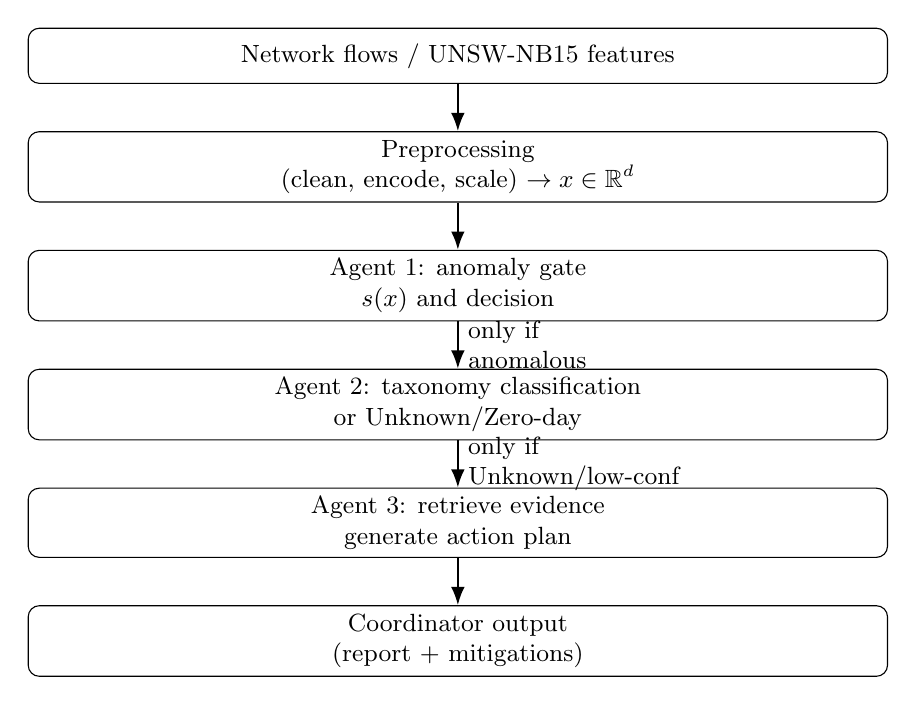
\begin{tikzpicture}[
  font=\small,
  node distance=6mm and 7mm,
  box/.style={draw, rounded corners, align=center, minimum height=7mm, inner sep=3pt, minimum width=0.9\columnwidth},
  arr/.style={-Latex, thick}
]
\node[box] (data) {Network flows / UNSW-NB15 features};
\node[box, below=of data] (prep) {Preprocessing\\(clean, encode, scale) $\rightarrow x\in\mathbb{R}^d$};
\node[box, below=of prep] (g1) {Agent 1: anomaly gate\\$s(x)$ and decision};
\node[box, below=of g1] (g2) {Agent 2: taxonomy classification\\or Unknown/Zero-day};
\node[box, below=of g2] (g3) {Agent 3: retrieve evidence\\generate action plan};
\node[box, below=of g3] (out) {Coordinator output\\(report + mitigations)};

\draw[arr] (data) -- (prep);
\draw[arr] (prep) -- (g1);
\draw[arr] (g1) -- node[right, align=left] {only if\\anomalous} (g2);
\draw[arr] (g2) -- node[right, align=left] {only if\\Unknown/low-conf} (g3);
\draw[arr] (g3) -- (out);
\end{tikzpicture}
\caption{Inference-time dataflow and selective escalation across agents.}
\label{fig:dataflow}
\end{figure}

\section{Methodology}
\subsection{Data Representation and Preprocessing}
We represent each network flow as a mixed-type feature vector including numerical, binary, and categorical attributes commonly used in IDS datasets (e.g., protocol, service, state, packet/byte counts, timing/rate statistics). A widely used benchmark for such settings is UNSW-NB15 \cite{moustafa2015unsw}, which includes a multi-class attack taxonomy.

Preprocessing is applied identically for training and inference:
\begin{itemize}
  \item \textbf{Cleaning and schema validation:} Remove invalid rows, handle missing values, and ensure consistent column schema.
  \item \textbf{Imputation:} Numerical features are imputed with mean/median/zero; categorical values with mode or an ``unknown'' token.
  \item \textbf{Categorical encoding:} Label encoding or one-hot encoding for categorical columns (e.g., protocol/service/state).
  \item \textbf{Scaling:} Standardization or min--max normalization for numerical columns to stabilize optimization.
  \item \textbf{Feature vector assembly:} Concatenate transformed features to obtain fixed-dimensional $x \in \mathbb{R}^d$.
\end{itemize}

\subsection{Agent~1: Autoencoder Training and Threshold Calibration}
\subsubsection{Architecture}
Agent~1 uses a symmetric multilayer perceptron autoencoder with encoder $f_\theta$ and decoder $g_\phi$:
\begin{equation}
  z = f_{\theta}(x),\quad \hat{x} = g_{\phi}(z).
\end{equation}
Hidden layers employ non-linear activations (e.g., LeakyReLU). Dropout and batch normalization may be used to improve generalization \cite{goodfellow2016dl}.

\subsubsection{Local objective and optimization}
Each client minimizes reconstruction loss over mini-batches $B$:
\begin{equation}
  \mathcal{L}_{AE}(\theta,\phi) = \frac{1}{|B|}\sum_{x\in B}\frac{1}{d}\lVert x - g_{\phi}(f_{\theta}(x)) \rVert_2^2.
\end{equation}
Optimization uses Adam with learning-rate scheduling and early stopping. The autoencoder is trained primarily on benign/normal traffic when available, consistent with anomaly detection practice \cite{chalapathy2019anomaly}.

\subsubsection{Threshold selection}
We calibrate the anomaly threshold $\tau$ using benign validation data:
\begin{equation}
  \tau = \mu_{benign} + k\sigma_{benign},
\end{equation}
or alternatively via a quantile (e.g., 0.95/0.99) of benign reconstruction errors. The calibration choice is reported and fixed before evaluation to avoid leakage.

\subsection{Federated Learning for Agent~1}
\subsubsection{Protocol}
We adopt the standard FL setting with $N$ clients. At each round $t$:
\begin{enumerate}
  \item The server broadcasts global parameters $w^t$.
  \item Each selected client $i$ performs $E$ local epochs on its private dataset and returns updated parameters $w_i^{t+1}$.
  \item The server aggregates using FedAvg:
  \begin{equation}
    w^{t+1} = \sum_{i=1}^{N} \frac{n_i}{\sum_j n_j} w_i^{t+1},
  \end{equation}
  where $n_i$ is the number of training samples at client $i$.
\end{enumerate}
FedAvg is widely adopted for communication-efficient decentralized training \cite{mcmahan2017fedavg}. A practical implementation can be orchestrated using Flower \cite{beutel2020flower}.

\subsubsection{Client heterogeneity}
Clients may have non-IID data (different traffic baselines, device mixes, and attack exposure). We account for this by (i) using weighted aggregation by $n_i$, (ii) reporting client participation, and (iii) optionally tuning $E$ and learning rate schedules to improve stability under heterogeneity \cite{kairouz2021flsurvey}.

\subsection{Privacy-Preserving Update Sharing (Optional)}
To reduce information leakage from model updates, we optionally apply a DP-inspired mechanism: per-layer (or per-tensor) clipping followed by additive Gaussian noise \cite{dwork2006dp,abadi2016dpsgd}.

Let $\Delta w$ be a client update (difference between local and global weights). Clipping with norm bound $C$:
\begin{equation}
  \Delta w \leftarrow \Delta w \cdot \min\left(1, \frac{C}{\lVert \Delta w \rVert_2}\right).
\end{equation}
Noise addition:
\begin{equation}
  \Delta w \leftarrow \Delta w + \mathcal{N}(0, \sigma^2 C^2 I).
\end{equation}
The server then aggregates noisy updates. For strict DP claims, we recommend using a formal accountant and reporting $(\varepsilon,\delta)$ under the chosen sampling and composition assumptions \cite{abadi2016dpsgd}.

\subsection{Agent~2: XGBoost Classification with Open-Set ``Unknown'' Handling}
\subsubsection{Model and training}
Agent~2 employs XGBoost for multi-class classification on tabular features \cite{xgboost2016}. The model outputs probability estimates $p(c\mid x)$ for classes in $\mathcal{C}$. Training minimizes multi-class log loss with regularization on tree complexity.

\subsubsection{Unknown/zero-day rule}
We apply Eq.~(\ref{eq:unknown_rule}) to detect low-confidence predictions and explicitly label them as Unknown/Zero-day. This is motivated by open set recognition, where the classifier must identify inputs not belonging to any known class \cite{scheirer2013openset,bendale2016openset}. In the proposed pipeline, Unknown outputs are prioritized for richer context retrieval and action planning.

\subsection{Agent~3: RAG-Based Action Planning}
\subsubsection{Knowledge base and retrieval}
We maintain a threat knowledge base consisting of:
\begin{itemize}
  \item MITRE ATT\&CK techniques, tactics, and procedure descriptions \cite{attck}
  \item CVE descriptions and vulnerability metadata \cite{cve}
  \item Incident response guidance and organizational playbooks (e.g., NIST IR) \cite{nist80061}
\end{itemize}
Documents are embedded and indexed for similarity search. For a query $q$, retrieval returns the top-$k$ passages $\{d_1,\dots,d_k\}$.

\subsubsection{Grounded generation}
Agent~3 prompts an LLM with retrieved context and the current detection summary. Retrieval-augmented generation reduces unsupported claims by conditioning outputs on explicit evidence \cite{lewis2020rag}. The LLM is instructed to output structured fields: severity, indicators, recommended actions, and references.

\subsubsection{Fallback behavior}
If retrieval or LLM access fails, Agent~3 returns a deterministic minimal set of mitigation steps based on severity and category to ensure operational continuity.

\subsection{Implementation Notes (Reproducibility-Oriented)}
To support reproducibility, the methodology recommends documenting:
\begin{itemize}
  \item Feature schema and preprocessing configuration (encoding, scaling).
  \item Agent~1 architecture (layer sizes, latent dimension, dropout/batch norm).
  \item FL hyperparameters (rounds, $E$, client fraction, optimizer, learning rate).
  \item DP parameters when used ($C$, $\sigma$, accountant configuration).
  \item Agent~2 hyperparameters (trees, depth, learning rate) and confidence threshold $\gamma$.
  \item Agent~3 retrieval configuration (embedding model, $k$, corpus sources) and prompting template.
\end{itemize}

% Optional: main novelty section as a separate include
% % FL + RAG Bridge Methodology (Novelty) — standalone section file
% Intended usage: % FL + RAG Bridge Methodology (Novelty) — standalone section file
% Intended usage: % FL + RAG Bridge Methodology (Novelty) — standalone section file
% Intended usage: \input{fl_rag_bridge_methodology.tex} from your main IEEEtran paper.

\section{Federated Learning--RAG Bridge Methodology (Main Novelty)}
\label{sec:fl-rag-bridge-methods}

This section formalizes the proposed \emph{Federated Learning--RAG Bridge} mechanism, which connects privacy-preserving global model evolution (from federated rounds) to improved, grounded threat explanations and action plans. The key idea is that the knowledge base (KB) does not ``learn new facts''; instead, the system learns to \emph{retrieve and present the right facts at the right time} as the global detection model changes.

\subsection{Motivation}
Federated learning improves detection models over time by aggregating decentralized updates without centralizing raw traffic. However, typical FL pipelines provide \emph{silent improvements}: detection accuracy changes, but the analyst-facing explanation layer remains static or purely local. In operational security, analysts require (i) evidence-backed context (e.g., MITRE ATT\&CK techniques, relevant CVEs), and (ii) actionable response steps.

The FL+RAG Bridge addresses this gap by monitoring global model updates and triggering targeted \emph{re-analysis} and \emph{explanation regeneration} for previously ambiguous or suspicious events. This design supports continuous knowledge transfer across organizations: once one client observes an attack pattern and contributes updates, other clients can benefit in subsequent rounds without sharing packets or logs.

\subsection{Bridge Interfaces and State}
\label{sec:bridge-interfaces}

The bridge maintains the following state across rounds:
\begin{itemize}
  \item \textbf{Round history:} a log of federated rounds, participating clients, update drift, and significance.
  \item \textbf{Previous global weights:} model snapshots used to compute drift between rounds.
  \item \textbf{Trigger queue:} pending trigger events requesting RAG re-analysis.
  \item \textbf{Explanation cache:} per-sample explanations keyed by (sample, round) to enable cross-round comparison.
\end{itemize}

The bridge connects to a coordinator that can (i) re-run analysis on queued samples and (ii) generate RAG-grounded explanations using the current KB + LLM.

\subsection{Update Semantics: From Weight Changes to Meaning}
\label{sec:update-semantics}

After each federated round $t$, the bridge receives a dictionary of model updates (e.g., autoencoder weights). It computes a normalized drift statistic between the previous global weights $w^{t-1}$ and new weights $w^{t}$.

For a set of parameter tensors $\{W_k\}$, a normalized per-tensor drift can be computed as:
\begin{equation}
\delta_k = \frac{\lVert W_k^{t} - W_k^{t-1} \rVert_2}{\lVert W_k^{t-1} \rVert_2 + \epsilon},
\end{equation}
with $\epsilon$ a small constant for numerical stability. The overall drift is aggregated (e.g., mean over $k$):
\begin{equation}
\Delta^{t} = \frac{1}{K}\sum_{k=1}^{K} \delta_k.
\end{equation}

\subsubsection{Significance levels}
To avoid ``always-on'' regeneration, the bridge discretizes drift into significance levels:
\begin{itemize}
  \item \textbf{Minimal:} $\Delta^{t} < 1\%$
  \item \textbf{Moderate:} $1\% \le \Delta^{t} < 5\%$
  \item \textbf{Significant:} $5\% \le \Delta^{t} < 15\%$
  \item \textbf{Major:} $\Delta^{t} \ge 15\%$
\end{itemize}
These thresholds are configurable; the methodology recommends fixing them before evaluation.

\subsection{Triggering Policy}
\label{sec:trigger-policy}

The bridge defines a trigger event $e^{t}$ when a round completes and the update significance is at least \emph{Moderate}. Each trigger event includes:
\begin{itemize}
  \item \textbf{Trigger type:} weight update / new pattern / confidence shift.
  \item \textbf{Round index:} $t$.
  \item \textbf{Affected categories:} categories most likely impacted by the update (for autoencoder, this may be ``all'').
  \item \textbf{Priority:} derived from significance (e.g., Major = highest priority).
\end{itemize}

The coordinator processes the trigger by re-analyzing a queue of samples collected from:
\begin{itemize}
  \item ``Unknown/Zero-day'' predictions from Agent~2 (low confidence),
  \item high anomaly scores from Agent~1,
  \item analyst-flagged suspicious flows.
\end{itemize}

\subsection{RAG Re-analysis and Explanation Regeneration}
\label{sec:rag-reanalysis}

For each queued sample $x$, the coordinator constructs a compact detection summary (category, confidence, anomaly flag/score, and any technique hints). The bridge then requests an explanation with federated context at round $t$.

\subsubsection{Retrieval step}
A query $q(x,t)$ is formed from the detection summary and routed to the KB vector index to retrieve top-$k$ passages $\{d_1,\dots,d_k\}$. Retrieval is designed to surface:
\begin{itemize}
  \item relevant MITRE ATT\&CK techniques and mitigations,
  \item related CVE references and IOCs,
  \item playbook-like response steps.
\end{itemize}

\subsubsection{Generation step}
The LLM is prompted with the retrieved context and instructed to output:
\begin{enumerate}
  \item a short threat summary,
  \item a \textbf{Recommended Actions} list ordered by priority,
  \item explicit CVE identifiers when applicable.
\end{enumerate}
RAG grounding is used to reduce unsupported claims and improve traceability \cite{lewis2020rag}.

\subsection{Cross-Round Comparison}
\label{sec:cross-round}

A key novelty is measuring how explanations evolve across rounds. For a sample $x$ and rounds $a<b$, the bridge can compare cached outputs:
\begin{itemize}
  \item confidence change $\Delta c = c^{b}-c^{a}$,
  \item change in ``zero-day'' status,
  \item changes in cited CVEs / techniques.
\end{itemize}
This enables a results section to show that federated learning improves not only detection but also the quality and specificity of analyst-facing explanations.

\subsection{Evaluation Metrics for the Bridge}
\label{sec:bridge-metrics}

We recommend reporting:
\begin{itemize}
  \item \textbf{Trigger dynamics:} number of trigger events per round; number of samples reprocessed.
  \item \textbf{Explanation quality vs rounds:} an aggregate score combining factuality proxies (valid CVE/ATT\&CK references), completeness (severity/indicators/actions), and specificity.
  \item \textbf{Zero-day explanation adequacy:} whether the explanation expresses appropriate uncertainty, compares to nearest known patterns, and provides investigation guidance.
  \item \textbf{Latency:} retrieval and generation latency distributions.
\end{itemize}

\subsection{Relationship to the Slide Concepts}
\label{sec:slide-mapping}

The bridge corresponds to the following conceptual claims (as illustrated in your slide deck):
\begin{itemize}
  \item \textbf{RAG Update Process:} improved global models trigger re-processing of queued suspicious samples and regeneration of explanations.
  \item \textbf{FL+RAG Bridge vs Traditional FL:} traditional FL improves detection silently, while the bridge ties model drift to explanation refresh.
  \item \textbf{Knowledge transfer via LOAO:} client-specific held-out attacks become detectable after several rounds without raw-data sharing.
\end{itemize}

% End of section
 from your main IEEEtran paper.

\section{Federated Learning--RAG Bridge Methodology (Main Novelty)}
\label{sec:fl-rag-bridge-methods}

This section formalizes the proposed \emph{Federated Learning--RAG Bridge} mechanism, which connects privacy-preserving global model evolution (from federated rounds) to improved, grounded threat explanations and action plans. The key idea is that the knowledge base (KB) does not ``learn new facts''; instead, the system learns to \emph{retrieve and present the right facts at the right time} as the global detection model changes.

\subsection{Motivation}
Federated learning improves detection models over time by aggregating decentralized updates without centralizing raw traffic. However, typical FL pipelines provide \emph{silent improvements}: detection accuracy changes, but the analyst-facing explanation layer remains static or purely local. In operational security, analysts require (i) evidence-backed context (e.g., MITRE ATT\&CK techniques, relevant CVEs), and (ii) actionable response steps.

The FL+RAG Bridge addresses this gap by monitoring global model updates and triggering targeted \emph{re-analysis} and \emph{explanation regeneration} for previously ambiguous or suspicious events. This design supports continuous knowledge transfer across organizations: once one client observes an attack pattern and contributes updates, other clients can benefit in subsequent rounds without sharing packets or logs.

\subsection{Bridge Interfaces and State}
\label{sec:bridge-interfaces}

The bridge maintains the following state across rounds:
\begin{itemize}
  \item \textbf{Round history:} a log of federated rounds, participating clients, update drift, and significance.
  \item \textbf{Previous global weights:} model snapshots used to compute drift between rounds.
  \item \textbf{Trigger queue:} pending trigger events requesting RAG re-analysis.
  \item \textbf{Explanation cache:} per-sample explanations keyed by (sample, round) to enable cross-round comparison.
\end{itemize}

The bridge connects to a coordinator that can (i) re-run analysis on queued samples and (ii) generate RAG-grounded explanations using the current KB + LLM.

\subsection{Update Semantics: From Weight Changes to Meaning}
\label{sec:update-semantics}

After each federated round $t$, the bridge receives a dictionary of model updates (e.g., autoencoder weights). It computes a normalized drift statistic between the previous global weights $w^{t-1}$ and new weights $w^{t}$.

For a set of parameter tensors $\{W_k\}$, a normalized per-tensor drift can be computed as:
\begin{equation}
\delta_k = \frac{\lVert W_k^{t} - W_k^{t-1} \rVert_2}{\lVert W_k^{t-1} \rVert_2 + \epsilon},
\end{equation}
with $\epsilon$ a small constant for numerical stability. The overall drift is aggregated (e.g., mean over $k$):
\begin{equation}
\Delta^{t} = \frac{1}{K}\sum_{k=1}^{K} \delta_k.
\end{equation}

\subsubsection{Significance levels}
To avoid ``always-on'' regeneration, the bridge discretizes drift into significance levels:
\begin{itemize}
  \item \textbf{Minimal:} $\Delta^{t} < 1\%$
  \item \textbf{Moderate:} $1\% \le \Delta^{t} < 5\%$
  \item \textbf{Significant:} $5\% \le \Delta^{t} < 15\%$
  \item \textbf{Major:} $\Delta^{t} \ge 15\%$
\end{itemize}
These thresholds are configurable; the methodology recommends fixing them before evaluation.

\subsection{Triggering Policy}
\label{sec:trigger-policy}

The bridge defines a trigger event $e^{t}$ when a round completes and the update significance is at least \emph{Moderate}. Each trigger event includes:
\begin{itemize}
  \item \textbf{Trigger type:} weight update / new pattern / confidence shift.
  \item \textbf{Round index:} $t$.
  \item \textbf{Affected categories:} categories most likely impacted by the update (for autoencoder, this may be ``all'').
  \item \textbf{Priority:} derived from significance (e.g., Major = highest priority).
\end{itemize}

The coordinator processes the trigger by re-analyzing a queue of samples collected from:
\begin{itemize}
  \item ``Unknown/Zero-day'' predictions from Agent~2 (low confidence),
  \item high anomaly scores from Agent~1,
  \item analyst-flagged suspicious flows.
\end{itemize}

\subsection{RAG Re-analysis and Explanation Regeneration}
\label{sec:rag-reanalysis}

For each queued sample $x$, the coordinator constructs a compact detection summary (category, confidence, anomaly flag/score, and any technique hints). The bridge then requests an explanation with federated context at round $t$.

\subsubsection{Retrieval step}
A query $q(x,t)$ is formed from the detection summary and routed to the KB vector index to retrieve top-$k$ passages $\{d_1,\dots,d_k\}$. Retrieval is designed to surface:
\begin{itemize}
  \item relevant MITRE ATT\&CK techniques and mitigations,
  \item related CVE references and IOCs,
  \item playbook-like response steps.
\end{itemize}

\subsubsection{Generation step}
The LLM is prompted with the retrieved context and instructed to output:
\begin{enumerate}
  \item a short threat summary,
  \item a \textbf{Recommended Actions} list ordered by priority,
  \item explicit CVE identifiers when applicable.
\end{enumerate}
RAG grounding is used to reduce unsupported claims and improve traceability \cite{lewis2020rag}.

\subsection{Cross-Round Comparison}
\label{sec:cross-round}

A key novelty is measuring how explanations evolve across rounds. For a sample $x$ and rounds $a<b$, the bridge can compare cached outputs:
\begin{itemize}
  \item confidence change $\Delta c = c^{b}-c^{a}$,
  \item change in ``zero-day'' status,
  \item changes in cited CVEs / techniques.
\end{itemize}
This enables a results section to show that federated learning improves not only detection but also the quality and specificity of analyst-facing explanations.

\subsection{Evaluation Metrics for the Bridge}
\label{sec:bridge-metrics}

We recommend reporting:
\begin{itemize}
  \item \textbf{Trigger dynamics:} number of trigger events per round; number of samples reprocessed.
  \item \textbf{Explanation quality vs rounds:} an aggregate score combining factuality proxies (valid CVE/ATT\&CK references), completeness (severity/indicators/actions), and specificity.
  \item \textbf{Zero-day explanation adequacy:} whether the explanation expresses appropriate uncertainty, compares to nearest known patterns, and provides investigation guidance.
  \item \textbf{Latency:} retrieval and generation latency distributions.
\end{itemize}

\subsection{Relationship to the Slide Concepts}
\label{sec:slide-mapping}

The bridge corresponds to the following conceptual claims (as illustrated in your slide deck):
\begin{itemize}
  \item \textbf{RAG Update Process:} improved global models trigger re-processing of queued suspicious samples and regeneration of explanations.
  \item \textbf{FL+RAG Bridge vs Traditional FL:} traditional FL improves detection silently, while the bridge ties model drift to explanation refresh.
  \item \textbf{Knowledge transfer via LOAO:} client-specific held-out attacks become detectable after several rounds without raw-data sharing.
\end{itemize}

% End of section
 from your main IEEEtran paper.

\section{Federated Learning--RAG Bridge Methodology (Main Novelty)}
\label{sec:fl-rag-bridge-methods}

This section formalizes the proposed \emph{Federated Learning--RAG Bridge} mechanism, which connects privacy-preserving global model evolution (from federated rounds) to improved, grounded threat explanations and action plans. The key idea is that the knowledge base (KB) does not ``learn new facts''; instead, the system learns to \emph{retrieve and present the right facts at the right time} as the global detection model changes.

\subsection{Motivation}
Federated learning improves detection models over time by aggregating decentralized updates without centralizing raw traffic. However, typical FL pipelines provide \emph{silent improvements}: detection accuracy changes, but the analyst-facing explanation layer remains static or purely local. In operational security, analysts require (i) evidence-backed context (e.g., MITRE ATT\&CK techniques, relevant CVEs), and (ii) actionable response steps.

The FL+RAG Bridge addresses this gap by monitoring global model updates and triggering targeted \emph{re-analysis} and \emph{explanation regeneration} for previously ambiguous or suspicious events. This design supports continuous knowledge transfer across organizations: once one client observes an attack pattern and contributes updates, other clients can benefit in subsequent rounds without sharing packets or logs.

\subsection{Bridge Interfaces and State}
\label{sec:bridge-interfaces}

The bridge maintains the following state across rounds:
\begin{itemize}
  \item \textbf{Round history:} a log of federated rounds, participating clients, update drift, and significance.
  \item \textbf{Previous global weights:} model snapshots used to compute drift between rounds.
  \item \textbf{Trigger queue:} pending trigger events requesting RAG re-analysis.
  \item \textbf{Explanation cache:} per-sample explanations keyed by (sample, round) to enable cross-round comparison.
\end{itemize}

The bridge connects to a coordinator that can (i) re-run analysis on queued samples and (ii) generate RAG-grounded explanations using the current KB + LLM.

\subsection{Update Semantics: From Weight Changes to Meaning}
\label{sec:update-semantics}

After each federated round $t$, the bridge receives a dictionary of model updates (e.g., autoencoder weights). It computes a normalized drift statistic between the previous global weights $w^{t-1}$ and new weights $w^{t}$.

For a set of parameter tensors $\{W_k\}$, a normalized per-tensor drift can be computed as:
\begin{equation}
\delta_k = \frac{\lVert W_k^{t} - W_k^{t-1} \rVert_2}{\lVert W_k^{t-1} \rVert_2 + \epsilon},
\end{equation}
with $\epsilon$ a small constant for numerical stability. The overall drift is aggregated (e.g., mean over $k$):
\begin{equation}
\Delta^{t} = \frac{1}{K}\sum_{k=1}^{K} \delta_k.
\end{equation}

\subsubsection{Significance levels}
To avoid ``always-on'' regeneration, the bridge discretizes drift into significance levels:
\begin{itemize}
  \item \textbf{Minimal:} $\Delta^{t} < 1\%$
  \item \textbf{Moderate:} $1\% \le \Delta^{t} < 5\%$
  \item \textbf{Significant:} $5\% \le \Delta^{t} < 15\%$
  \item \textbf{Major:} $\Delta^{t} \ge 15\%$
\end{itemize}
These thresholds are configurable; the methodology recommends fixing them before evaluation.

\subsection{Triggering Policy}
\label{sec:trigger-policy}

The bridge defines a trigger event $e^{t}$ when a round completes and the update significance is at least \emph{Moderate}. Each trigger event includes:
\begin{itemize}
  \item \textbf{Trigger type:} weight update / new pattern / confidence shift.
  \item \textbf{Round index:} $t$.
  \item \textbf{Affected categories:} categories most likely impacted by the update (for autoencoder, this may be ``all'').
  \item \textbf{Priority:} derived from significance (e.g., Major = highest priority).
\end{itemize}

The coordinator processes the trigger by re-analyzing a queue of samples collected from:
\begin{itemize}
  \item ``Unknown/Zero-day'' predictions from Agent~2 (low confidence),
  \item high anomaly scores from Agent~1,
  \item analyst-flagged suspicious flows.
\end{itemize}

\subsection{RAG Re-analysis and Explanation Regeneration}
\label{sec:rag-reanalysis}

For each queued sample $x$, the coordinator constructs a compact detection summary (category, confidence, anomaly flag/score, and any technique hints). The bridge then requests an explanation with federated context at round $t$.

\subsubsection{Retrieval step}
A query $q(x,t)$ is formed from the detection summary and routed to the KB vector index to retrieve top-$k$ passages $\{d_1,\dots,d_k\}$. Retrieval is designed to surface:
\begin{itemize}
  \item relevant MITRE ATT\&CK techniques and mitigations,
  \item related CVE references and IOCs,
  \item playbook-like response steps.
\end{itemize}

\subsubsection{Generation step}
The LLM is prompted with the retrieved context and instructed to output:
\begin{enumerate}
  \item a short threat summary,
  \item a \textbf{Recommended Actions} list ordered by priority,
  \item explicit CVE identifiers when applicable.
\end{enumerate}
RAG grounding is used to reduce unsupported claims and improve traceability \cite{lewis2020rag}.

\subsection{Cross-Round Comparison}
\label{sec:cross-round}

A key novelty is measuring how explanations evolve across rounds. For a sample $x$ and rounds $a<b$, the bridge can compare cached outputs:
\begin{itemize}
  \item confidence change $\Delta c = c^{b}-c^{a}$,
  \item change in ``zero-day'' status,
  \item changes in cited CVEs / techniques.
\end{itemize}
This enables a results section to show that federated learning improves not only detection but also the quality and specificity of analyst-facing explanations.

\subsection{Evaluation Metrics for the Bridge}
\label{sec:bridge-metrics}

We recommend reporting:
\begin{itemize}
  \item \textbf{Trigger dynamics:} number of trigger events per round; number of samples reprocessed.
  \item \textbf{Explanation quality vs rounds:} an aggregate score combining factuality proxies (valid CVE/ATT\&CK references), completeness (severity/indicators/actions), and specificity.
  \item \textbf{Zero-day explanation adequacy:} whether the explanation expresses appropriate uncertainty, compares to nearest known patterns, and provides investigation guidance.
  \item \textbf{Latency:} retrieval and generation latency distributions.
\end{itemize}

\subsection{Relationship to the Slide Concepts}
\label{sec:slide-mapping}

The bridge corresponds to the following conceptual claims (as illustrated in your slide deck):
\begin{itemize}
  \item \textbf{RAG Update Process:} improved global models trigger re-processing of queued suspicious samples and regeneration of explanations.
  \item \textbf{FL+RAG Bridge vs Traditional FL:} traditional FL improves detection silently, while the bridge ties model drift to explanation refresh.
  \item \textbf{Knowledge transfer via LOAO:} client-specific held-out attacks become detectable after several rounds without raw-data sharing.
\end{itemize}

% End of section


% Optional: system architecture section as a separate include
% % System Architecture (copy-paste ready)
% Intended usage: % System Architecture (copy-paste ready)
% Intended usage: % System Architecture (copy-paste ready)
% Intended usage: \input{system_architecture_proposed_framework.tex} from an IEEEtran main paper.
%
% Requires the following packages in the main preamble:
%   \usepackage{amsmath,amssymb}
%   \usepackage{hyperref}
%   \usepackage{xurl}
%   \usepackage{tikz}
%   \usetikzlibrary{arrows.meta,positioning,fit,shapes.geometric}
%
% Notes:
% - This section is intentionally high-level; it describes connectivity and roles.
% - Detailed agent internals (losses, hyperparameters, training procedures) belong in the Methodology section.

\section{System Architecture of the Proposed Framework}
\label{sec:system_architecture}

This section presents the overall architecture of the proposed three-agent framework and how its components interact during (i) federated training and (ii) inference-time decision making. The design follows a \emph{hierarchical offloading} principle: inexpensive detection runs first, and only uncertain or high-risk cases escalate to more expensive reasoning.

\subsection{Top-Level Components}
The system consists of five logical components:
\begin{itemize}
  \item \textbf{Data plane (network flows):} Raw traffic is summarized into flow-level records and transformed into a fixed-dimensional feature vector $x\in\mathbb{R}^d$ using a consistent preprocessing pipeline.
  \item \textbf{Agent~1 (Federated anomaly gate):} An unsupervised autoencoder produces an anomaly score $s(x)$ and filters likely-benign traffic early. To respect privacy constraints across sites, Agent~1 is trained using federated averaging (FedAvg) across clients, without centralizing raw data \cite{mcmahan2017fedavg,kairouz2021flsurvey}.
  \item \textbf{Agent~2 (Known-attack classifier + Unknown mode):} A supervised gradient-boosted tree model predicts a known taxonomy label when confidence is sufficient; otherwise it outputs \emph{Unknown/Zero-day} to avoid forced misclassification under distribution shift \cite{chen2016xgboost,scheirer2013openset,bendale2016openmax}.
  \item \textbf{Agent~3 (RAG+LLM action planner):} A retrieval-augmented generation (RAG) module retrieves relevant threat-intelligence evidence and prompts an LLM to produce a structured analyst-facing action plan grounded in the retrieved context \cite{lewis2020rag,nist80061,mitreattack,mitrecve}.
  \item \textbf{Coordinator (orchestrator):} The coordinator applies routing logic, executes the staged pipeline, and assembles a unified incident report (scores, labels, retrieved evidence, and recommended actions).
\end{itemize}

\subsection{Connectivity and Selective Escalation}
Most flows terminate at Agent~1 as benign. Only flows exceeding the anomaly threshold are forwarded to Agent~2 for taxonomy classification. Agent~3 is invoked sparingly for cases that are most costly to resolve automatically: low-confidence predictions, explicit Unknown/Zero-day outputs, or incidents requiring contextual enrichment (e.g., mapping to ATT\&CK techniques and mitigations).

\textbf{Operational routing.} For a preprocessed flow vector $x$:
\begin{enumerate}
  \item Agent~1 computes $s(x)$ and returns a gate decision (benign vs. suspicious).
  \item If suspicious, Agent~2 returns a predicted class $\hat{c}$ and confidence $c(x)$; if $c(x)$ falls below a threshold $\gamma$, it outputs \emph{Unknown/Zero-day} \cite{scheirer2013openset}.
  \item The coordinator invokes Agent~3 when Agent~2 returns Unknown or confidence is low, producing a grounded summary and mitigation plan.
\end{enumerate}

\subsection{Federated Learning Placement and Purpose}
Federated learning is placed at Agent~1 to improve the generality of the anomaly gate across non-IID client environments while preserving privacy. Clients train locally on private traffic, and an FL server aggregates updates into a global model using FedAvg \cite{mcmahan2017fedavg}. This placement is deliberate: parameter averaging is straightforward for neural networks, whereas federated learning for tree ensembles typically requires specialized protocols beyond simple averaging \cite{kairouz2021flsurvey}. Therefore, in this framework we \emph{claim FL for Agent~1 only}.

\subsection{Fed--RAG Bridge: Purpose and Role}
The Fed--RAG bridge links the evolving federated detector (Agent~1) to the knowledge-grounded reasoning layer (Agent~3). Its purpose is twofold:
\begin{itemize}
  \item \textbf{Explainability alignment:} As Agent~1 updates across rounds, the distribution of anomaly scores and the ``shape'' of flagged traffic can drift. The bridge ensures that operator-facing explanations remain consistent with the current detector behavior.
  \item \textbf{Evidence refresh under drift/novelty:} When federated-round metadata indicates significant drift (e.g., shifts in reconstruction-error statistics or threshold movement), the bridge triggers re-analysis and refreshes the retrieval context used by Agent~3, improving actionability under emerging threats.
\end{itemize}

\begin{figure*}[t]
\centering
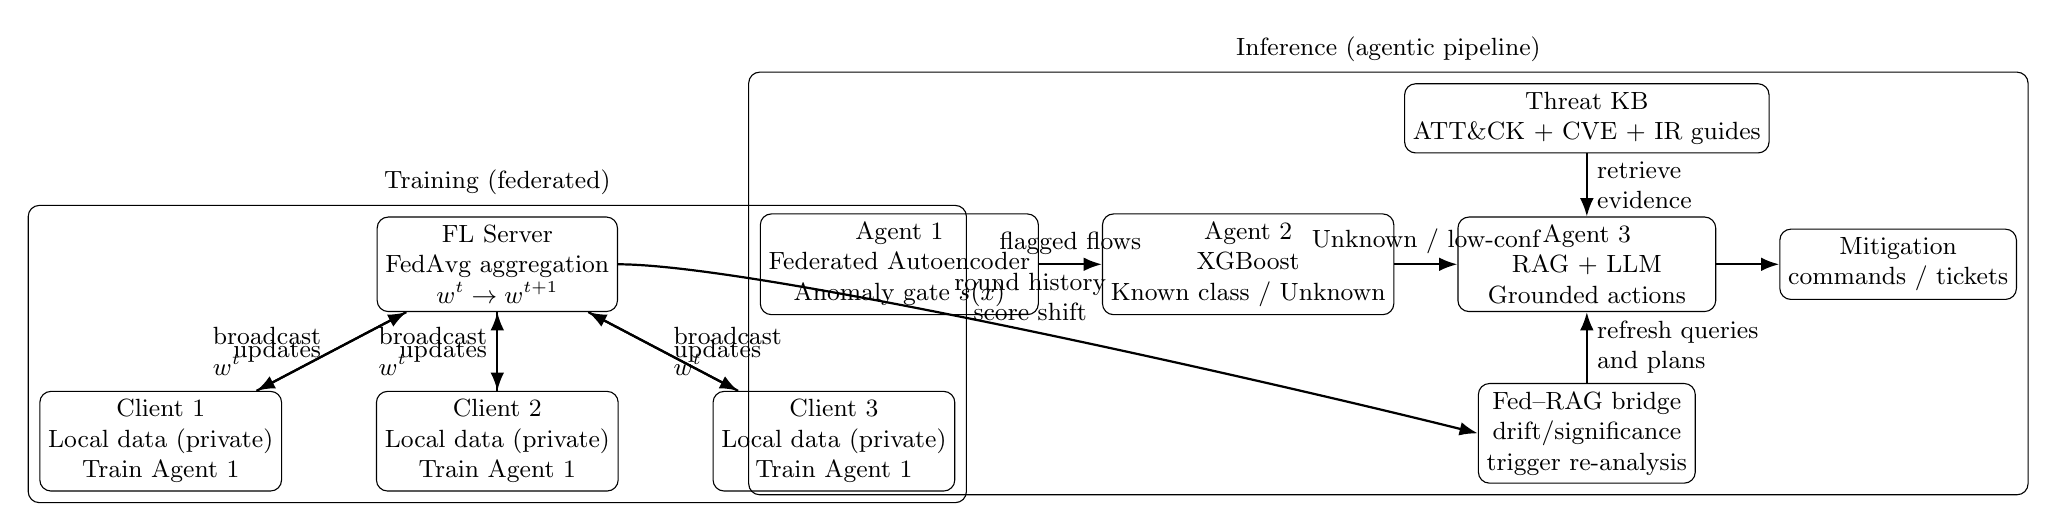
\begin{tikzpicture}[
  font=\small,
  node distance=7mm and 9mm,
  box/.style={draw, rounded corners, align=center, minimum height=7mm, inner sep=3pt},
  bigbox/.style={box, minimum width=0.27\textwidth},
  sbox/.style={box, minimum width=0.19\textwidth},
  arr/.style={-Latex, thick}
]

% --- Training side (FL) ---
\node[box, minimum width=0.23\textwidth] (flsrv) {FL Server\\FedAvg aggregation\\$w^{t}\rightarrow w^{t+1}$};
\node[sbox, below left=10mm and 12mm of flsrv] (c1) {Client 1\\Local data (private)\\Train Agent 1};
\node[sbox, below=10mm of flsrv] (c2) {Client 2\\Local data (private)\\Train Agent 1};
\node[sbox, below right=10mm and 12mm of flsrv] (c3) {Client 3\\Local data (private)\\Train Agent 1};

\draw[arr] (flsrv) -- node[left, align=left] {broadcast\\$w^t$} (c1);
\draw[arr] (flsrv) -- node[left, align=left] {broadcast\\$w^t$} (c2);
\draw[arr] (flsrv) -- node[right, align=left] {broadcast\\$w^t$} (c3);

\draw[arr] (c1) -- node[left, align=left] {updates} (flsrv);
\draw[arr] (c2) -- node[left, align=left] {updates} (flsrv);
\draw[arr] (c3) -- node[right, align=left] {updates} (flsrv);

% --- Inference side (pipeline) ---
\node[bigbox, right=18mm of flsrv] (a1) {Agent 1\\Federated Autoencoder\\Anomaly gate $s(x)$};
\node[bigbox, right=8mm of a1] (a2) {Agent 2\\XGBoost\\Known class / Unknown};
\node[bigbox, right=8mm of a2] (a3) {Agent 3\\RAG + LLM\\Grounded actions};
\node[box, right=8mm of a3, minimum width=0.18\textwidth] (mit) {Mitigation\\commands / tickets};

\node[box, above=8mm of a3, minimum width=0.22\textwidth] (kb) {Threat KB\\ATT\&CK + CVE + IR guides};

\draw[arr] (a1) -- node[above] {flagged flows} (a2);
\draw[arr] (a2) -- node[above] {Unknown / low-conf} (a3);
\draw[arr] (a3) -- (mit);
\draw[arr] (kb) -- node[right, align=left] {retrieve\\evidence} (a3);

% --- Bridge ---
\node[box, below=9mm of a3, minimum width=0.22\textwidth] (bridge) {Fed--RAG bridge\\drift/significance\\trigger re-analysis};
\draw[arr] (flsrv.east) .. controls +(18mm,0mm) and +(-24mm,6mm) .. node[above, align=center] {round history\\score shift} (bridge.west);
\draw[arr] (bridge.north) -- node[right, align=left] {refresh queries\\and plans} (a3.south);

\node[fit=(flsrv)(c1)(c2)(c3), draw, rounded corners, inner sep=4pt, label={[font=\small]above:Training (federated)}] {};
\node[fit=(a1)(a2)(a3)(kb)(bridge)(mit), draw, rounded corners, inner sep=4pt, label={[font=\small]above:Inference (agentic pipeline)}] {};

\end{tikzpicture}
\caption{Overall system architecture: federated training for Agent~1 only, hierarchical inference across three agents, and a Fed--RAG bridge that refreshes retrieval and explanations when the anomaly profile drifts.}
\label{fig:overall_architecture}
\end{figure*}

\begin{figure}[t]
\centering
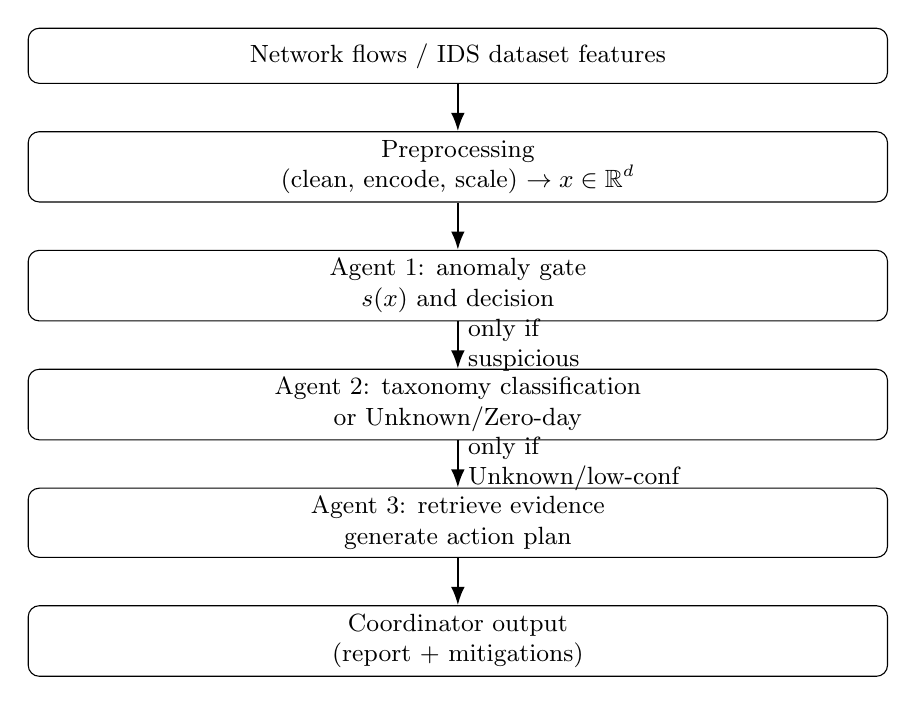
\begin{tikzpicture}[
  font=\small,
  node distance=6mm and 7mm,
  box/.style={draw, rounded corners, align=center, minimum height=7mm, inner sep=3pt, minimum width=0.9\columnwidth},
  arr/.style={-Latex, thick}
]
\node[box] (data) {Network flows / IDS dataset features};
\node[box, below=of data] (prep) {Preprocessing\\(clean, encode, scale) $\rightarrow x\in\mathbb{R}^d$};
\node[box, below=of prep] (g1) {Agent 1: anomaly gate\\$s(x)$ and decision};
\node[box, below=of g1] (g2) {Agent 2: taxonomy classification\\or Unknown/Zero-day};
\node[box, below=of g2] (g3) {Agent 3: retrieve evidence\\generate action plan};
\node[box, below=of g3] (out) {Coordinator output\\(report + mitigations)};

\draw[arr] (data) -- (prep);
\draw[arr] (prep) -- (g1);
\draw[arr] (g1) -- node[right, align=left] {only if\\suspicious} (g2);
\draw[arr] (g2) -- node[right, align=left] {only if\\Unknown/low-conf} (g3);
\draw[arr] (g3) -- (out);
\end{tikzpicture}
\caption{Inference-time dataflow and selective escalation across agents.}
\label{fig:dataflow}
\end{figure}

% -----------------------------
% References for this standalone architecture section.
% If your main paper uses BibTeX, move these \bibitem entries into your .bib
% and remove this thebibliography environment.
\begin{thebibliography}{99}
\bibitem{mcmahan2017fedavg}
B.~McMahan, E.~Moore, D.~Ramage, S.~Hampson, and B.~A. y~Arcas, ``Communication-Efficient Learning of Deep Networks from Decentralized Data,'' in \emph{Proc. AISTATS}, 2017.

\bibitem{kairouz2021flsurvey}
P.~Kairouz \emph{et al.}, ``Advances and Open Problems in Federated Learning,'' \emph{Foundations and Trends in Machine Learning}, vol.~14, no.~1--2, pp.~1--210, 2021.

\bibitem{chen2016xgboost}
T.~Chen and C.~Guestrin, ``XGBoost: A Scalable Tree Boosting System,'' in \emph{Proc. ACM SIGKDD}, 2016, pp.~785--794.

\bibitem{scheirer2013openset}
W.~J. Scheirer, A.~Rocha, R.~J. Micheals, and T.~E. Boult, ``Toward Open Set Recognition,'' \emph{IEEE Trans. Pattern Anal. Mach. Intell.}, vol.~35, no.~7, pp.~1757--1772, 2013.

\bibitem{bendale2016openmax}
A.~Bendale and T.~E. Boult, ``Towards Open Set Deep Networks,'' in \emph{Proc. CVPR}, 2016.

\bibitem{lewis2020rag}
P.~Lewis \emph{et al.}, ``Retrieval-Augmented Generation for Knowledge-Intensive NLP Tasks,'' in \emph{Proc. NeurIPS}, 2020.

\bibitem{nist80061}
K.~Scarfone, P.~Mell, A.~Souppaya, and M.~Olsen, ``Computer Security Incident Handling Guide,'' NIST Special Publication 800-61 Revision 2, 2012.

\bibitem{mitreattack}
MITRE, ``MITRE ATT\&CK,'' 2026. [Online]. Available: \url{https://attack.mitre.org/}. Accessed: Apr. 19, 2026.

\bibitem{mitrecve}
MITRE, ``Common Vulnerabilities and Exposures (CVE),'' 2026. [Online]. Available: \url{https://www.cve.org/}. Accessed: Apr. 19, 2026.
\end{thebibliography}
 from an IEEEtran main paper.
%
% Requires the following packages in the main preamble:
%   \usepackage{amsmath,amssymb}
%   \usepackage{hyperref}
%   \usepackage{xurl}
%   \usepackage{tikz}
%   \usetikzlibrary{arrows.meta,positioning,fit,shapes.geometric}
%
% Notes:
% - This section is intentionally high-level; it describes connectivity and roles.
% - Detailed agent internals (losses, hyperparameters, training procedures) belong in the Methodology section.

\section{System Architecture of the Proposed Framework}
\label{sec:system_architecture}

This section presents the overall architecture of the proposed three-agent framework and how its components interact during (i) federated training and (ii) inference-time decision making. The design follows a \emph{hierarchical offloading} principle: inexpensive detection runs first, and only uncertain or high-risk cases escalate to more expensive reasoning.

\subsection{Top-Level Components}
The system consists of five logical components:
\begin{itemize}
  \item \textbf{Data plane (network flows):} Raw traffic is summarized into flow-level records and transformed into a fixed-dimensional feature vector $x\in\mathbb{R}^d$ using a consistent preprocessing pipeline.
  \item \textbf{Agent~1 (Federated anomaly gate):} An unsupervised autoencoder produces an anomaly score $s(x)$ and filters likely-benign traffic early. To respect privacy constraints across sites, Agent~1 is trained using federated averaging (FedAvg) across clients, without centralizing raw data \cite{mcmahan2017fedavg,kairouz2021flsurvey}.
  \item \textbf{Agent~2 (Known-attack classifier + Unknown mode):} A supervised gradient-boosted tree model predicts a known taxonomy label when confidence is sufficient; otherwise it outputs \emph{Unknown/Zero-day} to avoid forced misclassification under distribution shift \cite{chen2016xgboost,scheirer2013openset,bendale2016openmax}.
  \item \textbf{Agent~3 (RAG+LLM action planner):} A retrieval-augmented generation (RAG) module retrieves relevant threat-intelligence evidence and prompts an LLM to produce a structured analyst-facing action plan grounded in the retrieved context \cite{lewis2020rag,nist80061,mitreattack,mitrecve}.
  \item \textbf{Coordinator (orchestrator):} The coordinator applies routing logic, executes the staged pipeline, and assembles a unified incident report (scores, labels, retrieved evidence, and recommended actions).
\end{itemize}

\subsection{Connectivity and Selective Escalation}
Most flows terminate at Agent~1 as benign. Only flows exceeding the anomaly threshold are forwarded to Agent~2 for taxonomy classification. Agent~3 is invoked sparingly for cases that are most costly to resolve automatically: low-confidence predictions, explicit Unknown/Zero-day outputs, or incidents requiring contextual enrichment (e.g., mapping to ATT\&CK techniques and mitigations).

\textbf{Operational routing.} For a preprocessed flow vector $x$:
\begin{enumerate}
  \item Agent~1 computes $s(x)$ and returns a gate decision (benign vs. suspicious).
  \item If suspicious, Agent~2 returns a predicted class $\hat{c}$ and confidence $c(x)$; if $c(x)$ falls below a threshold $\gamma$, it outputs \emph{Unknown/Zero-day} \cite{scheirer2013openset}.
  \item The coordinator invokes Agent~3 when Agent~2 returns Unknown or confidence is low, producing a grounded summary and mitigation plan.
\end{enumerate}

\subsection{Federated Learning Placement and Purpose}
Federated learning is placed at Agent~1 to improve the generality of the anomaly gate across non-IID client environments while preserving privacy. Clients train locally on private traffic, and an FL server aggregates updates into a global model using FedAvg \cite{mcmahan2017fedavg}. This placement is deliberate: parameter averaging is straightforward for neural networks, whereas federated learning for tree ensembles typically requires specialized protocols beyond simple averaging \cite{kairouz2021flsurvey}. Therefore, in this framework we \emph{claim FL for Agent~1 only}.

\subsection{Fed--RAG Bridge: Purpose and Role}
The Fed--RAG bridge links the evolving federated detector (Agent~1) to the knowledge-grounded reasoning layer (Agent~3). Its purpose is twofold:
\begin{itemize}
  \item \textbf{Explainability alignment:} As Agent~1 updates across rounds, the distribution of anomaly scores and the ``shape'' of flagged traffic can drift. The bridge ensures that operator-facing explanations remain consistent with the current detector behavior.
  \item \textbf{Evidence refresh under drift/novelty:} When federated-round metadata indicates significant drift (e.g., shifts in reconstruction-error statistics or threshold movement), the bridge triggers re-analysis and refreshes the retrieval context used by Agent~3, improving actionability under emerging threats.
\end{itemize}

\begin{figure*}[t]
\centering
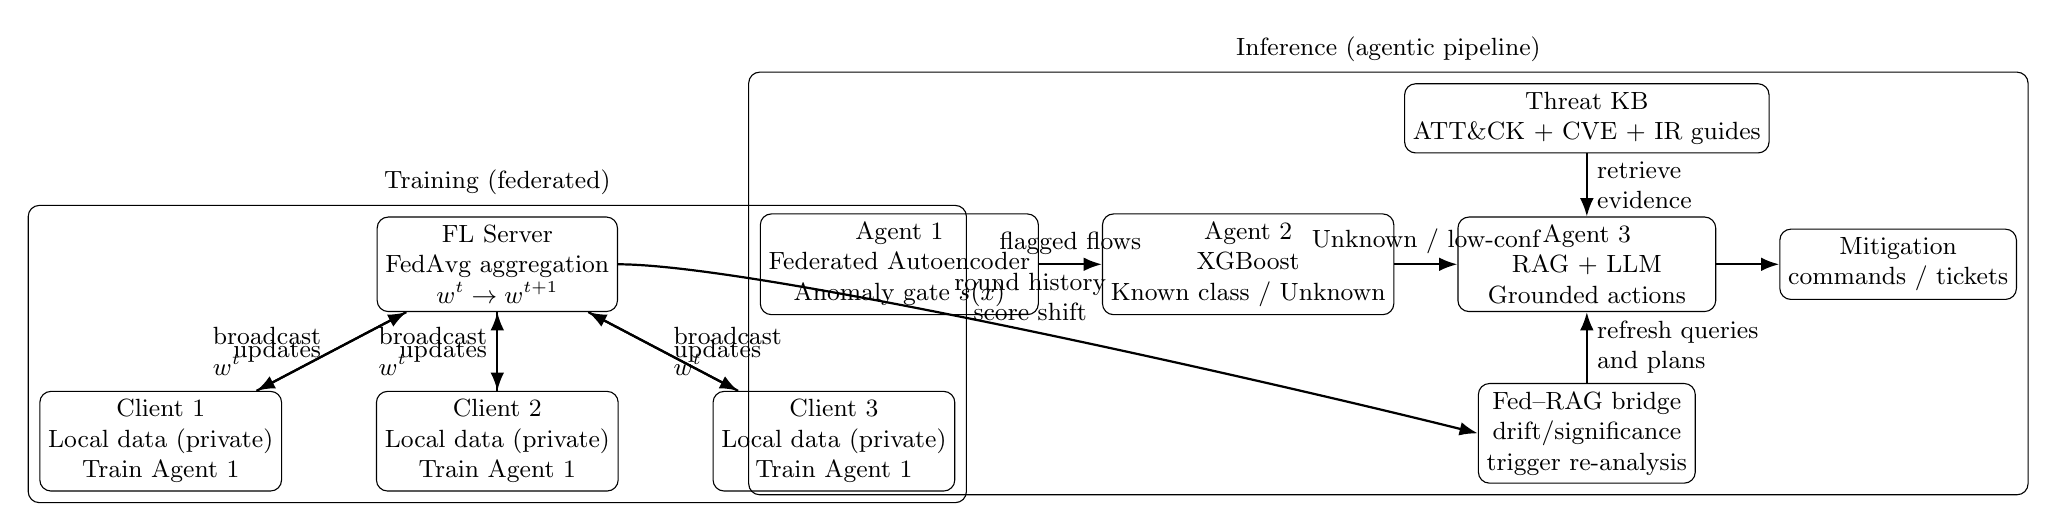
\begin{tikzpicture}[
  font=\small,
  node distance=7mm and 9mm,
  box/.style={draw, rounded corners, align=center, minimum height=7mm, inner sep=3pt},
  bigbox/.style={box, minimum width=0.27\textwidth},
  sbox/.style={box, minimum width=0.19\textwidth},
  arr/.style={-Latex, thick}
]

% --- Training side (FL) ---
\node[box, minimum width=0.23\textwidth] (flsrv) {FL Server\\FedAvg aggregation\\$w^{t}\rightarrow w^{t+1}$};
\node[sbox, below left=10mm and 12mm of flsrv] (c1) {Client 1\\Local data (private)\\Train Agent 1};
\node[sbox, below=10mm of flsrv] (c2) {Client 2\\Local data (private)\\Train Agent 1};
\node[sbox, below right=10mm and 12mm of flsrv] (c3) {Client 3\\Local data (private)\\Train Agent 1};

\draw[arr] (flsrv) -- node[left, align=left] {broadcast\\$w^t$} (c1);
\draw[arr] (flsrv) -- node[left, align=left] {broadcast\\$w^t$} (c2);
\draw[arr] (flsrv) -- node[right, align=left] {broadcast\\$w^t$} (c3);

\draw[arr] (c1) -- node[left, align=left] {updates} (flsrv);
\draw[arr] (c2) -- node[left, align=left] {updates} (flsrv);
\draw[arr] (c3) -- node[right, align=left] {updates} (flsrv);

% --- Inference side (pipeline) ---
\node[bigbox, right=18mm of flsrv] (a1) {Agent 1\\Federated Autoencoder\\Anomaly gate $s(x)$};
\node[bigbox, right=8mm of a1] (a2) {Agent 2\\XGBoost\\Known class / Unknown};
\node[bigbox, right=8mm of a2] (a3) {Agent 3\\RAG + LLM\\Grounded actions};
\node[box, right=8mm of a3, minimum width=0.18\textwidth] (mit) {Mitigation\\commands / tickets};

\node[box, above=8mm of a3, minimum width=0.22\textwidth] (kb) {Threat KB\\ATT\&CK + CVE + IR guides};

\draw[arr] (a1) -- node[above] {flagged flows} (a2);
\draw[arr] (a2) -- node[above] {Unknown / low-conf} (a3);
\draw[arr] (a3) -- (mit);
\draw[arr] (kb) -- node[right, align=left] {retrieve\\evidence} (a3);

% --- Bridge ---
\node[box, below=9mm of a3, minimum width=0.22\textwidth] (bridge) {Fed--RAG bridge\\drift/significance\\trigger re-analysis};
\draw[arr] (flsrv.east) .. controls +(18mm,0mm) and +(-24mm,6mm) .. node[above, align=center] {round history\\score shift} (bridge.west);
\draw[arr] (bridge.north) -- node[right, align=left] {refresh queries\\and plans} (a3.south);

\node[fit=(flsrv)(c1)(c2)(c3), draw, rounded corners, inner sep=4pt, label={[font=\small]above:Training (federated)}] {};
\node[fit=(a1)(a2)(a3)(kb)(bridge)(mit), draw, rounded corners, inner sep=4pt, label={[font=\small]above:Inference (agentic pipeline)}] {};

\end{tikzpicture}
\caption{Overall system architecture: federated training for Agent~1 only, hierarchical inference across three agents, and a Fed--RAG bridge that refreshes retrieval and explanations when the anomaly profile drifts.}
\label{fig:overall_architecture}
\end{figure*}

\begin{figure}[t]
\centering
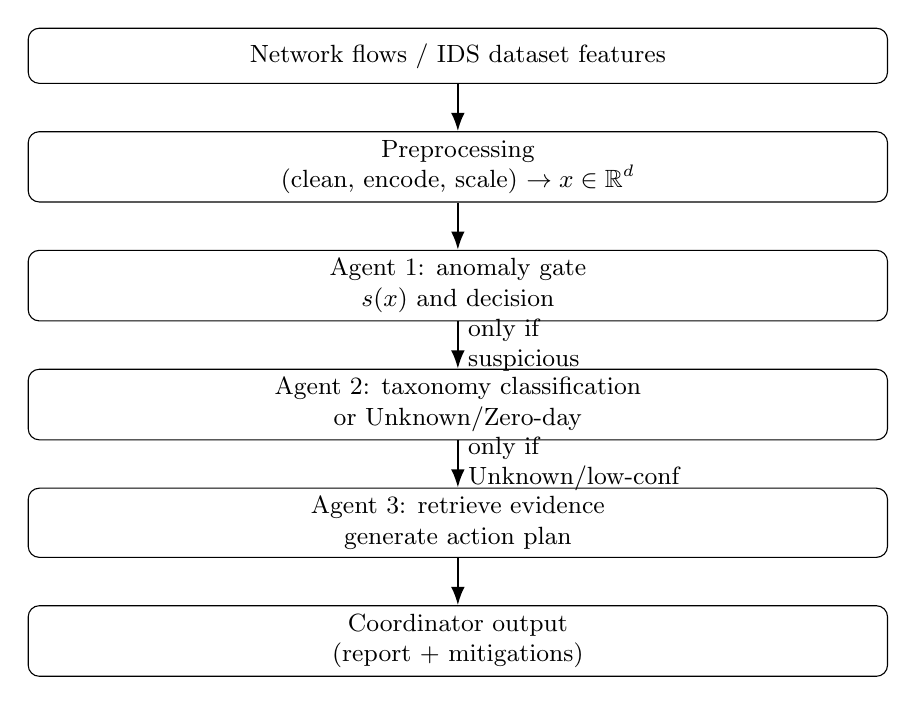
\begin{tikzpicture}[
  font=\small,
  node distance=6mm and 7mm,
  box/.style={draw, rounded corners, align=center, minimum height=7mm, inner sep=3pt, minimum width=0.9\columnwidth},
  arr/.style={-Latex, thick}
]
\node[box] (data) {Network flows / IDS dataset features};
\node[box, below=of data] (prep) {Preprocessing\\(clean, encode, scale) $\rightarrow x\in\mathbb{R}^d$};
\node[box, below=of prep] (g1) {Agent 1: anomaly gate\\$s(x)$ and decision};
\node[box, below=of g1] (g2) {Agent 2: taxonomy classification\\or Unknown/Zero-day};
\node[box, below=of g2] (g3) {Agent 3: retrieve evidence\\generate action plan};
\node[box, below=of g3] (out) {Coordinator output\\(report + mitigations)};

\draw[arr] (data) -- (prep);
\draw[arr] (prep) -- (g1);
\draw[arr] (g1) -- node[right, align=left] {only if\\suspicious} (g2);
\draw[arr] (g2) -- node[right, align=left] {only if\\Unknown/low-conf} (g3);
\draw[arr] (g3) -- (out);
\end{tikzpicture}
\caption{Inference-time dataflow and selective escalation across agents.}
\label{fig:dataflow}
\end{figure}

% -----------------------------
% References for this standalone architecture section.
% If your main paper uses BibTeX, move these \bibitem entries into your .bib
% and remove this thebibliography environment.
\begin{thebibliography}{99}
\bibitem{mcmahan2017fedavg}
B.~McMahan, E.~Moore, D.~Ramage, S.~Hampson, and B.~A. y~Arcas, ``Communication-Efficient Learning of Deep Networks from Decentralized Data,'' in \emph{Proc. AISTATS}, 2017.

\bibitem{kairouz2021flsurvey}
P.~Kairouz \emph{et al.}, ``Advances and Open Problems in Federated Learning,'' \emph{Foundations and Trends in Machine Learning}, vol.~14, no.~1--2, pp.~1--210, 2021.

\bibitem{chen2016xgboost}
T.~Chen and C.~Guestrin, ``XGBoost: A Scalable Tree Boosting System,'' in \emph{Proc. ACM SIGKDD}, 2016, pp.~785--794.

\bibitem{scheirer2013openset}
W.~J. Scheirer, A.~Rocha, R.~J. Micheals, and T.~E. Boult, ``Toward Open Set Recognition,'' \emph{IEEE Trans. Pattern Anal. Mach. Intell.}, vol.~35, no.~7, pp.~1757--1772, 2013.

\bibitem{bendale2016openmax}
A.~Bendale and T.~E. Boult, ``Towards Open Set Deep Networks,'' in \emph{Proc. CVPR}, 2016.

\bibitem{lewis2020rag}
P.~Lewis \emph{et al.}, ``Retrieval-Augmented Generation for Knowledge-Intensive NLP Tasks,'' in \emph{Proc. NeurIPS}, 2020.

\bibitem{nist80061}
K.~Scarfone, P.~Mell, A.~Souppaya, and M.~Olsen, ``Computer Security Incident Handling Guide,'' NIST Special Publication 800-61 Revision 2, 2012.

\bibitem{mitreattack}
MITRE, ``MITRE ATT\&CK,'' 2026. [Online]. Available: \url{https://attack.mitre.org/}. Accessed: Apr. 19, 2026.

\bibitem{mitrecve}
MITRE, ``Common Vulnerabilities and Exposures (CVE),'' 2026. [Online]. Available: \url{https://www.cve.org/}. Accessed: Apr. 19, 2026.
\end{thebibliography}
 from an IEEEtran main paper.
%
% Requires the following packages in the main preamble:
%   \usepackage{amsmath,amssymb}
%   \usepackage{hyperref}
%   \usepackage{xurl}
%   \usepackage{tikz}
%   \usetikzlibrary{arrows.meta,positioning,fit,shapes.geometric}
%
% Notes:
% - This section is intentionally high-level; it describes connectivity and roles.
% - Detailed agent internals (losses, hyperparameters, training procedures) belong in the Methodology section.

\section{System Architecture of the Proposed Framework}
\label{sec:system_architecture}

This section presents the overall architecture of the proposed three-agent framework and how its components interact during (i) federated training and (ii) inference-time decision making. The design follows a \emph{hierarchical offloading} principle: inexpensive detection runs first, and only uncertain or high-risk cases escalate to more expensive reasoning.

\subsection{Top-Level Components}
The system consists of five logical components:
\begin{itemize}
  \item \textbf{Data plane (network flows):} Raw traffic is summarized into flow-level records and transformed into a fixed-dimensional feature vector $x\in\mathbb{R}^d$ using a consistent preprocessing pipeline.
  \item \textbf{Agent~1 (Federated anomaly gate):} An unsupervised autoencoder produces an anomaly score $s(x)$ and filters likely-benign traffic early. To respect privacy constraints across sites, Agent~1 is trained using federated averaging (FedAvg) across clients, without centralizing raw data \cite{mcmahan2017fedavg,kairouz2021flsurvey}.
  \item \textbf{Agent~2 (Known-attack classifier + Unknown mode):} A supervised gradient-boosted tree model predicts a known taxonomy label when confidence is sufficient; otherwise it outputs \emph{Unknown/Zero-day} to avoid forced misclassification under distribution shift \cite{chen2016xgboost,scheirer2013openset,bendale2016openmax}.
  \item \textbf{Agent~3 (RAG+LLM action planner):} A retrieval-augmented generation (RAG) module retrieves relevant threat-intelligence evidence and prompts an LLM to produce a structured analyst-facing action plan grounded in the retrieved context \cite{lewis2020rag,nist80061,mitreattack,mitrecve}.
  \item \textbf{Coordinator (orchestrator):} The coordinator applies routing logic, executes the staged pipeline, and assembles a unified incident report (scores, labels, retrieved evidence, and recommended actions).
\end{itemize}

\subsection{Connectivity and Selective Escalation}
Most flows terminate at Agent~1 as benign. Only flows exceeding the anomaly threshold are forwarded to Agent~2 for taxonomy classification. Agent~3 is invoked sparingly for cases that are most costly to resolve automatically: low-confidence predictions, explicit Unknown/Zero-day outputs, or incidents requiring contextual enrichment (e.g., mapping to ATT\&CK techniques and mitigations).

\textbf{Operational routing.} For a preprocessed flow vector $x$:
\begin{enumerate}
  \item Agent~1 computes $s(x)$ and returns a gate decision (benign vs. suspicious).
  \item If suspicious, Agent~2 returns a predicted class $\hat{c}$ and confidence $c(x)$; if $c(x)$ falls below a threshold $\gamma$, it outputs \emph{Unknown/Zero-day} \cite{scheirer2013openset}.
  \item The coordinator invokes Agent~3 when Agent~2 returns Unknown or confidence is low, producing a grounded summary and mitigation plan.
\end{enumerate}

\subsection{Federated Learning Placement and Purpose}
Federated learning is placed at Agent~1 to improve the generality of the anomaly gate across non-IID client environments while preserving privacy. Clients train locally on private traffic, and an FL server aggregates updates into a global model using FedAvg \cite{mcmahan2017fedavg}. This placement is deliberate: parameter averaging is straightforward for neural networks, whereas federated learning for tree ensembles typically requires specialized protocols beyond simple averaging \cite{kairouz2021flsurvey}. Therefore, in this framework we \emph{claim FL for Agent~1 only}.

\subsection{Fed--RAG Bridge: Purpose and Role}
The Fed--RAG bridge links the evolving federated detector (Agent~1) to the knowledge-grounded reasoning layer (Agent~3). Its purpose is twofold:
\begin{itemize}
  \item \textbf{Explainability alignment:} As Agent~1 updates across rounds, the distribution of anomaly scores and the ``shape'' of flagged traffic can drift. The bridge ensures that operator-facing explanations remain consistent with the current detector behavior.
  \item \textbf{Evidence refresh under drift/novelty:} When federated-round metadata indicates significant drift (e.g., shifts in reconstruction-error statistics or threshold movement), the bridge triggers re-analysis and refreshes the retrieval context used by Agent~3, improving actionability under emerging threats.
\end{itemize}

\begin{figure*}[t]
\centering
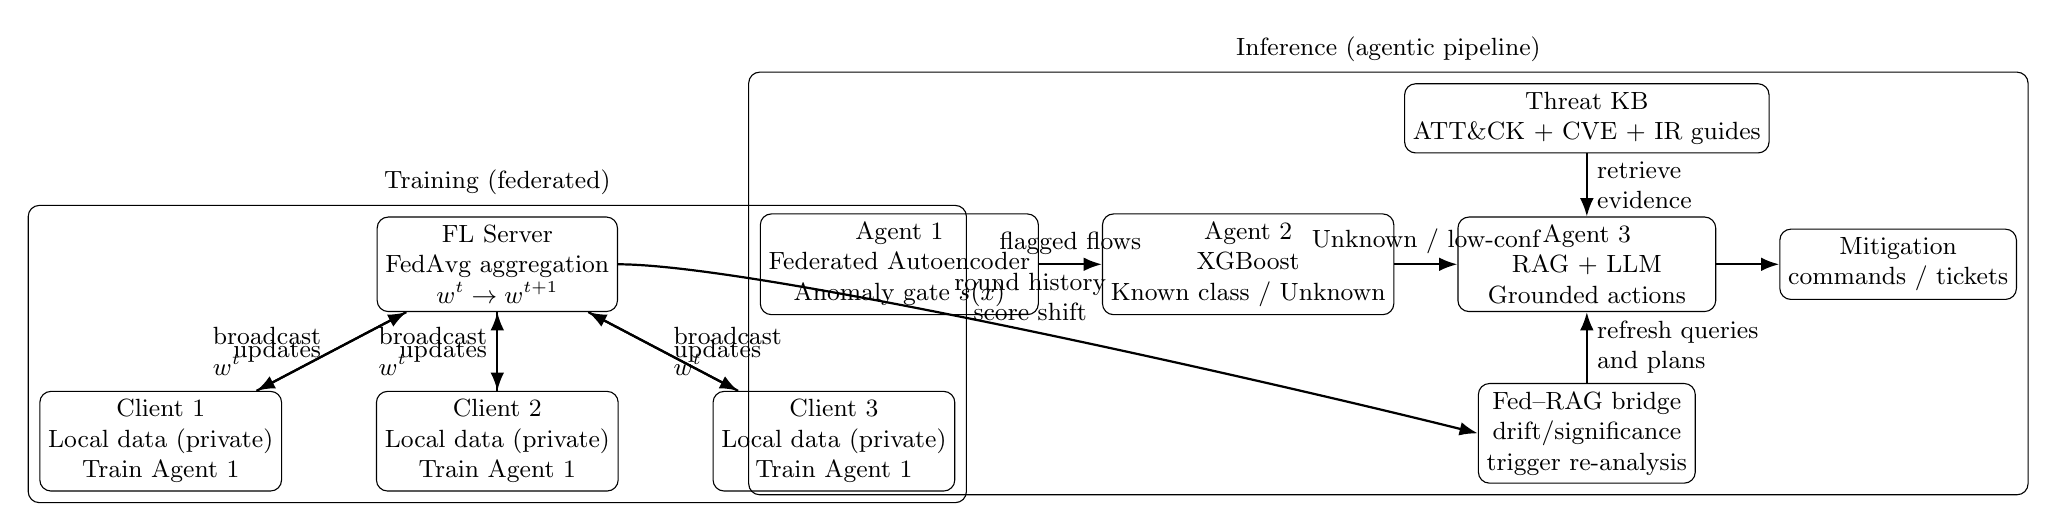
\begin{tikzpicture}[
  font=\small,
  node distance=7mm and 9mm,
  box/.style={draw, rounded corners, align=center, minimum height=7mm, inner sep=3pt},
  bigbox/.style={box, minimum width=0.27\textwidth},
  sbox/.style={box, minimum width=0.19\textwidth},
  arr/.style={-Latex, thick}
]

% --- Training side (FL) ---
\node[box, minimum width=0.23\textwidth] (flsrv) {FL Server\\FedAvg aggregation\\$w^{t}\rightarrow w^{t+1}$};
\node[sbox, below left=10mm and 12mm of flsrv] (c1) {Client 1\\Local data (private)\\Train Agent 1};
\node[sbox, below=10mm of flsrv] (c2) {Client 2\\Local data (private)\\Train Agent 1};
\node[sbox, below right=10mm and 12mm of flsrv] (c3) {Client 3\\Local data (private)\\Train Agent 1};

\draw[arr] (flsrv) -- node[left, align=left] {broadcast\\$w^t$} (c1);
\draw[arr] (flsrv) -- node[left, align=left] {broadcast\\$w^t$} (c2);
\draw[arr] (flsrv) -- node[right, align=left] {broadcast\\$w^t$} (c3);

\draw[arr] (c1) -- node[left, align=left] {updates} (flsrv);
\draw[arr] (c2) -- node[left, align=left] {updates} (flsrv);
\draw[arr] (c3) -- node[right, align=left] {updates} (flsrv);

% --- Inference side (pipeline) ---
\node[bigbox, right=18mm of flsrv] (a1) {Agent 1\\Federated Autoencoder\\Anomaly gate $s(x)$};
\node[bigbox, right=8mm of a1] (a2) {Agent 2\\XGBoost\\Known class / Unknown};
\node[bigbox, right=8mm of a2] (a3) {Agent 3\\RAG + LLM\\Grounded actions};
\node[box, right=8mm of a3, minimum width=0.18\textwidth] (mit) {Mitigation\\commands / tickets};

\node[box, above=8mm of a3, minimum width=0.22\textwidth] (kb) {Threat KB\\ATT\&CK + CVE + IR guides};

\draw[arr] (a1) -- node[above] {flagged flows} (a2);
\draw[arr] (a2) -- node[above] {Unknown / low-conf} (a3);
\draw[arr] (a3) -- (mit);
\draw[arr] (kb) -- node[right, align=left] {retrieve\\evidence} (a3);

% --- Bridge ---
\node[box, below=9mm of a3, minimum width=0.22\textwidth] (bridge) {Fed--RAG bridge\\drift/significance\\trigger re-analysis};
\draw[arr] (flsrv.east) .. controls +(18mm,0mm) and +(-24mm,6mm) .. node[above, align=center] {round history\\score shift} (bridge.west);
\draw[arr] (bridge.north) -- node[right, align=left] {refresh queries\\and plans} (a3.south);

\node[fit=(flsrv)(c1)(c2)(c3), draw, rounded corners, inner sep=4pt, label={[font=\small]above:Training (federated)}] {};
\node[fit=(a1)(a2)(a3)(kb)(bridge)(mit), draw, rounded corners, inner sep=4pt, label={[font=\small]above:Inference (agentic pipeline)}] {};

\end{tikzpicture}
\caption{Overall system architecture: federated training for Agent~1 only, hierarchical inference across three agents, and a Fed--RAG bridge that refreshes retrieval and explanations when the anomaly profile drifts.}
\label{fig:overall_architecture}
\end{figure*}

\begin{figure}[t]
\centering
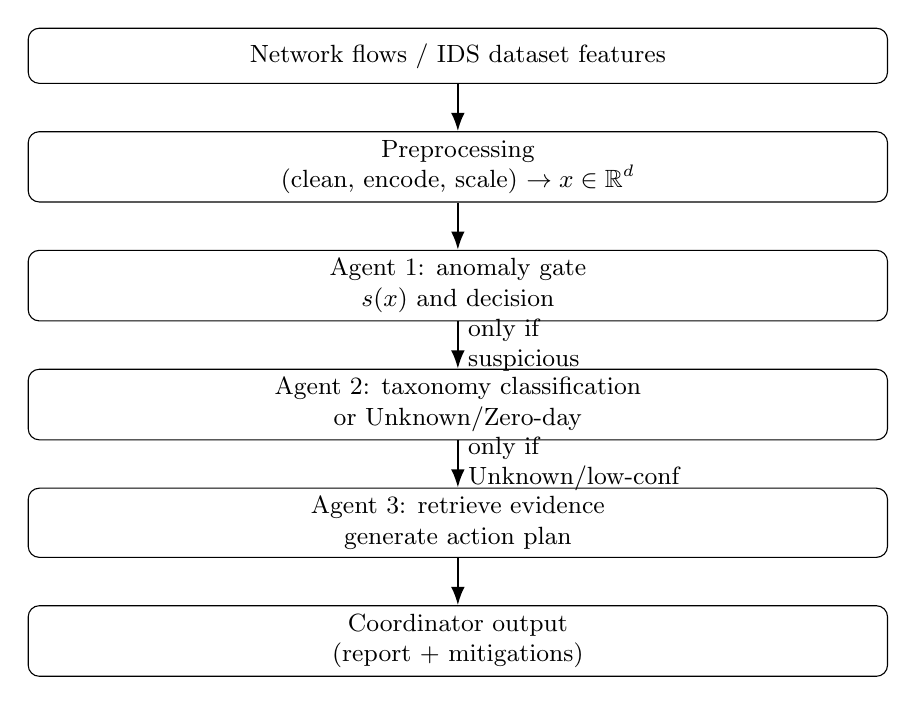
\begin{tikzpicture}[
  font=\small,
  node distance=6mm and 7mm,
  box/.style={draw, rounded corners, align=center, minimum height=7mm, inner sep=3pt, minimum width=0.9\columnwidth},
  arr/.style={-Latex, thick}
]
\node[box] (data) {Network flows / IDS dataset features};
\node[box, below=of data] (prep) {Preprocessing\\(clean, encode, scale) $\rightarrow x\in\mathbb{R}^d$};
\node[box, below=of prep] (g1) {Agent 1: anomaly gate\\$s(x)$ and decision};
\node[box, below=of g1] (g2) {Agent 2: taxonomy classification\\or Unknown/Zero-day};
\node[box, below=of g2] (g3) {Agent 3: retrieve evidence\\generate action plan};
\node[box, below=of g3] (out) {Coordinator output\\(report + mitigations)};

\draw[arr] (data) -- (prep);
\draw[arr] (prep) -- (g1);
\draw[arr] (g1) -- node[right, align=left] {only if\\suspicious} (g2);
\draw[arr] (g2) -- node[right, align=left] {only if\\Unknown/low-conf} (g3);
\draw[arr] (g3) -- (out);
\end{tikzpicture}
\caption{Inference-time dataflow and selective escalation across agents.}
\label{fig:dataflow}
\end{figure}

% -----------------------------
% References for this standalone architecture section.
% If your main paper uses BibTeX, move these \bibitem entries into your .bib
% and remove this thebibliography environment.
\begin{thebibliography}{99}
\bibitem{mcmahan2017fedavg}
B.~McMahan, E.~Moore, D.~Ramage, S.~Hampson, and B.~A. y~Arcas, ``Communication-Efficient Learning of Deep Networks from Decentralized Data,'' in \emph{Proc. AISTATS}, 2017.

\bibitem{kairouz2021flsurvey}
P.~Kairouz \emph{et al.}, ``Advances and Open Problems in Federated Learning,'' \emph{Foundations and Trends in Machine Learning}, vol.~14, no.~1--2, pp.~1--210, 2021.

\bibitem{chen2016xgboost}
T.~Chen and C.~Guestrin, ``XGBoost: A Scalable Tree Boosting System,'' in \emph{Proc. ACM SIGKDD}, 2016, pp.~785--794.

\bibitem{scheirer2013openset}
W.~J. Scheirer, A.~Rocha, R.~J. Micheals, and T.~E. Boult, ``Toward Open Set Recognition,'' \emph{IEEE Trans. Pattern Anal. Mach. Intell.}, vol.~35, no.~7, pp.~1757--1772, 2013.

\bibitem{bendale2016openmax}
A.~Bendale and T.~E. Boult, ``Towards Open Set Deep Networks,'' in \emph{Proc. CVPR}, 2016.

\bibitem{lewis2020rag}
P.~Lewis \emph{et al.}, ``Retrieval-Augmented Generation for Knowledge-Intensive NLP Tasks,'' in \emph{Proc. NeurIPS}, 2020.

\bibitem{nist80061}
K.~Scarfone, P.~Mell, A.~Souppaya, and M.~Olsen, ``Computer Security Incident Handling Guide,'' NIST Special Publication 800-61 Revision 2, 2012.

\bibitem{mitreattack}
MITRE, ``MITRE ATT\&CK,'' 2026. [Online]. Available: \url{https://attack.mitre.org/}. Accessed: Apr. 19, 2026.

\bibitem{mitrecve}
MITRE, ``Common Vulnerabilities and Exposures (CVE),'' 2026. [Online]. Available: \url{https://www.cve.org/}. Accessed: Apr. 19, 2026.
\end{thebibliography}


% Optional: detailed three-agent methodology as a separate include
% % Methodology (copy-paste ready)
% Intended usage: % Methodology (copy-paste ready)
% Intended usage: % Methodology (copy-paste ready)
% Intended usage: \input{methodology_three_agents.tex} from an IEEEtran main paper.
% Required packages in main preamble: amsmath, amssymb, graphicx, booktabs, siunitx, tikz.
% TikZ libraries recommended: \usetikzlibrary{positioning,arrows.meta}
% If you compile standalone, wrap this in an IEEEtran document and include the bibliography.

\section{Methodology}
\label{sec:methodology}

We propose a hierarchical, three-agent intrusion detection and response pipeline that balances (i) real-time filtering, (ii) accurate attack-family classification, and (iii) grounded analyst-facing action planning. The design follows a progressive offloading strategy: low-cost models handle the full traffic stream, while expensive reasoning is invoked only for ambiguous or high-risk events. This is aligned with practical intrusion detection deployments, where early-stage filters reduce throughput to downstream analysis stages \cite{Mirsky2018Kitsune}.

\subsection{Data Preparation and Preprocessing}
\label{sec:data_preparation}

This section describes dataset selection, splits, cleaning, feature engineering, and preprocessing. These steps precede the three agents and ensure that all models operate on consistent feature representations.

\subsubsection{Dataset selection and files}
\textbf{Primary benchmark.} We use UNSW-NB15 as the main benchmark dataset for network intrusion detection, due to its diversity of attack types and its structured feature representation \cite{Moustafa2015UNSW,Moustafa2015UNSW2}.

\textbf{Structured train/test splits.} We use the official structured CSV files:
\begin{itemize}
  \item \emph{Training:} \texttt{UNSW\_NB15\_training-set.csv}
  \item \emph{Testing:} \texttt{UNSW\_NB15\_testing-set.csv}
\end{itemize}

\textbf{Raw distribution evaluation.} To approximate ``in-the-wild'' distributions and validate robustness, we additionally evaluate on the raw UNSW-NB15 split files (\texttt{UNSW-NB15\_1.csv} to \texttt{UNSW-NB15\_4.csv}). These files contain the same 49 columns but do not include headers and may differ in column ordering; therefore we load them with an explicit schema to avoid column-mismatch errors.

\subsubsection{Loading, schema alignment, and cleaning}
We implement dataset ingestion using modular components (a \emph{DataLoader} for loading/initial cleaning and a \emph{Preprocessor} for normalization and encoding). This modularity supports reproducibility and simplifies extending to additional datasets.

\textbf{Schema alignment for raw files.} For raw files without headers, we use a dedicated loader that assigns the 49 column names explicitly (47 features plus \texttt{attack\_cat} and \texttt{label}) and normalizes label fields:
\begin{itemize}
  \item Missing or empty \texttt{attack\_cat} values are mapped to \emph{Normal}.
  \item The binary \texttt{label} field is coerced to integer, where 0 indicates normal and 1 indicates attack.
  \item Category strings are stripped and standardized (e.g., minor whitespace variants are normalized).
\end{itemize}

\textbf{Missing values and numeric coercion.} We treat missing values and invalid numeric fields using robust conversions (coerce-to-numeric followed by imputation). In the general preprocessing pipeline, we use simple imputers (median for numeric features and mode for categorical features) to avoid dropping flows and to preserve deployment realism \cite{Pedregosa2011Scikit}.

\subsubsection{Feature engineering}
We compute derived features that improve separability and capture traffic dynamics. In particular, we compute the connection rate:
\begin{equation}
\texttt{rate} = \frac{\texttt{spkts}+\texttt{dpkts}}{\texttt{dur}+\epsilon},
\end{equation}
with $\epsilon>0$ to avoid division by zero. All engineered features are computed deterministically and are included consistently across train/test and raw evaluation.

\subsubsection{Normalization and encoding}
\textbf{Numerical scaling.} We apply min--max scaling to numerical features, matching the default configuration used by the pipeline. Min--max scaling is particularly suitable for autoencoders, where feature ranges can dominate reconstruction loss if left unnormalized. Our implementation uses standard preprocessing utilities (e.g., \texttt{MinMaxScaler}) \cite{Pedregosa2011Scikit}.

\textbf{Categorical encoding.} Categorical columns (e.g., \texttt{proto}, \texttt{service}, \texttt{state}) are encoded either via integer factorization (label encoding) or via one-hot encoding depending on the experiment configuration. In our baseline, we use label encoding to keep the feature dimensionality stable and to simplify deployment.

\subsubsection{Sampling and reproducibility}
To enable fair comparisons across models, we use fixed random seeds (e.g., \texttt{random\_state}=42) for sampling and train/test splits. All preprocessing artifacts (scaler parameters, encoders, and imputers) are fit on the training split and reused unchanged for validation/test transformations, preventing leakage.

\textbf{Class-imbalance handling for supervised training.} UNSW-NB15 exhibits class imbalance (normal traffic dominates, while some attack categories are rare). For Agent~2 training, we apply SMOTE oversampling \emph{only on the training split} after preprocessing to improve minority-class recall while keeping evaluation unbiased \cite{Chawla2002SMOTE}.

\subsection{Pipeline Overview and Decision Flow}
\label{sec:method_overview}

Let $x \in \mathbb{R}^d$ denote a network-flow feature vector extracted from raw packets (e.g., connection statistics, byte/packet counts, TTL/state features, and aggregate temporal features). We follow the feature format provided by standard IDS benchmarks such as UNSW-NB15 \cite{Moustafa2015UNSW}.

The pipeline produces:
\begin{itemize}
  \item a gate decision (Normal vs Anomalous),
  \item a threat category label among known classes, optionally with an ``Unknown/Zero-day'' flag,
  \item a grounded, structured action plan (recommended actions, relevant ATT\&CK techniques, and candidate CVEs when applicable).
\end{itemize}

\textbf{Preprocessing.} For Agents 1 and 2, tabular features are standardized using statistics computed on the training split (mean/variance scaling). Categorical features (if present) are one-hot encoded. The anomaly score produced by Agent 1 is appended to the Agent 2 feature vector to provide a consistent signal of ``distance from normality''.

\textbf{Hierarchical offloading policy.} The system executes:
\begin{enumerate}
  \item \textbf{Agent 1 (Autoencoder gate):} compute anomaly score $s(x)$ and decide $g(x)\in\{\text{Normal},\text{Anomalous}\}$.
  \item \textbf{Agent 2 (XGBoost classifier):} if $g(x)=\text{Anomalous}$, predict class probabilities $p(y\mid x)$ over $K$ known categories and a confidence score $c(x)=\max_y p(y\mid x)$.
  \item \textbf{Agent 3 (RAG+LLM action planner):} if $c(x)<\gamma$ (low confidence) or if Agent 2 explicitly flags ``Unknown/Zero-day'', retrieve threat-intelligence context and generate an action plan.
\end{enumerate}

\textbf{Rationale.} Agent 1 is optimized for high recall and low latency, ensuring that potentially malicious traffic is not missed. Agent 2 provides a low-cost categorical interpretation to support automated response policies for known threats. Agent 3 is invoked selectively to (i) explain uncertain events and (ii) provide grounded response actions using external threat intelligence, reducing hallucinations relative to purely parametric generation \cite{Lewis2020RAG}.

\begin{figure}[t]
\centering
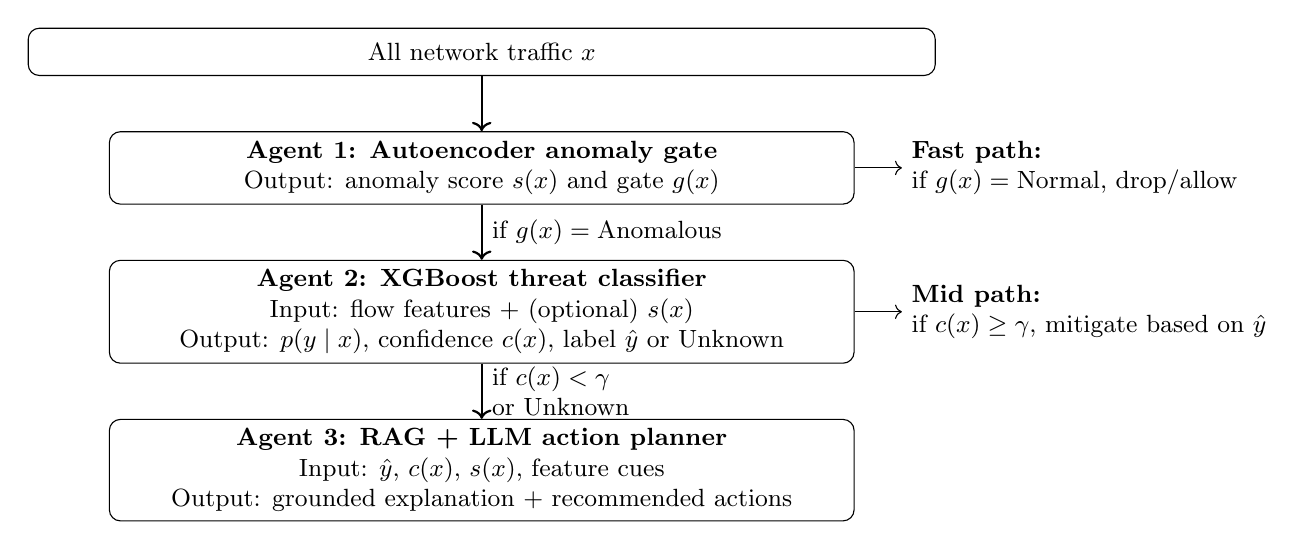
\begin{tikzpicture}[node distance=7mm, font=\small]
  \node[draw, rounded corners, align=center, minimum width=0.95\columnwidth, minimum height=6mm] (traffic) {All network traffic $x$};

  \node[draw, rounded corners, align=center, below=of traffic, minimum width=0.78\columnwidth] (a1) {\textbf{Agent 1: Autoencoder anomaly gate}\\
  Output: anomaly score $s(x)$ and gate $g(x)$};

  \node[draw, rounded corners, align=center, below=of a1, minimum width=0.78\columnwidth] (a2) {\textbf{Agent 2: XGBoost threat classifier}\\
  Input: flow features + (optional) $s(x)$\\
  Output: $p(y\mid x)$, confidence $c(x)$, label $\hat{y}$ or Unknown};

  \node[draw, rounded corners, align=center, below=of a2, minimum width=0.78\columnwidth] (a3) {\textbf{Agent 3: RAG + LLM action planner}\\
  Input: $\hat{y}$, $c(x)$, $s(x)$, feature cues\\
  Output: grounded explanation + recommended actions};

  \draw[->, thick] (traffic) -- (a1);
  \draw[->, thick] (a1) -- node[right, align=left] {if $g(x)=\text{Anomalous}$} (a2);
  \draw[->, thick] (a2) -- node[right, align=left] {if $c(x)<\gamma$\\or Unknown} (a3);

  \node[align=left, right=6mm of a1] (drop) {\textbf{Fast path:}\\if $g(x)=\text{Normal}$, drop/allow};
  \draw[->] (a1.east) -- (drop.west);

  \node[align=left, right=6mm of a2] (mit) {\textbf{Mid path:}\\if $c(x)\ge\gamma$, mitigate based on $\hat{y}$};
  \draw[->] (a2.east) -- (mit.west);
\end{tikzpicture}
\caption{Hierarchical offloading decision flow for the three-agent pipeline.}
\label{fig:hierarchical_offloading}
\end{figure}

\subsection{Agent 1: Autoencoder Anomaly Detector (Gate)}
\label{sec:agent1_method}

\subsubsection{Model architecture}
Agent 1 is a feed-forward PyTorch autoencoder trained to reconstruct benign-dominant traffic. The architecture follows a symmetric bottleneck design (input dimension $d=40$):
\begin{equation}
40 \rightarrow 32 \rightarrow 16 \rightarrow 8 \rightarrow 16 \rightarrow 32 \rightarrow 40,
\end{equation}
where the bottleneck encourages compression into a low-dimensional latent representation. Autoencoders are widely used for anomaly detection by learning normal patterns and flagging reconstruction deviations \cite{Hinton2006Reducing,Mirsky2018Kitsune}.

\textbf{Training objective.} The autoencoder is trained to minimize reconstruction loss on the training split, dominated by Normal traffic:
\begin{equation}
 \min_\theta\; \mathbb{E}_{x\sim\mathcal{D}_{\text{train}}}\left[\lVert x - f_\theta(x)\rVert_2^2\right].
\end{equation}
We use mini-batch optimization (Adam) with early stopping based on validation loss to prevent overfitting.

\subsubsection{Anomaly scoring}
Let $f_\theta(\cdot)$ denote the autoencoder reconstruction function. The anomaly score is computed as the mean squared reconstruction error:
\begin{equation}
 s(x) = \frac{1}{d}\lVert x - f_\theta(x) \rVert_2^2.
\end{equation}
The gate decision is:
\begin{equation}
 g(x) = \mathbb{I}[s(x) \ge \tau],
\end{equation}
where $\tau$ is calibrated on a validation split to achieve a target recall/false-positive trade-off. We select $\tau$ using either (i) a quantile rule on Normal reconstruction errors or (ii) a validation sweep to maximize attack recall at an acceptable false-positive rate.

\textbf{Operating point.} Since the system is designed to avoid missing attacks, we bias $\tau$ toward high recall even if it increases false positives; downstream agents and RAG-based reasoning mitigate the cost by handling only escalated flows.

\subsubsection{Confidence signal}
We additionally expose a normalized confidence proxy derived from the distance to the threshold:
\begin{equation}
 \kappa(x) = \sigma\left(\alpha\,(s(x)-\tau)\right),
\end{equation}
where $\sigma$ is a logistic function and $\alpha$ controls steepness. This scalar is used (i) as an auxiliary feature for Agent 2 to improve separability and (ii) as an escalation cue to Agent 3 when confidence is low.

\subsection{Agent 2: XGBoost Threat Classifier}
\label{sec:agent2_method}

Agent 2 performs supervised multi-class classification over $K=10$ categories (Normal plus nine attack families). We use gradient-boosted decision trees due to their strong performance on tabular intrusion datasets and low inference latency \cite{Chen2016XGBoost}.

\subsubsection{Input features}
For flows flagged anomalous by Agent 1, Agent 2 receives:
\begin{itemize}
  \item raw flow features $x$,
  \item the anomaly score $s(x)$ (or confidence proxy $\kappa(x)$) from Agent 1,
  \item optional engineered statistics (e.g., z-scored feature groups).
\end{itemize}

\textbf{Feature fusion.} The anomaly score acts as a global indicator of deviation from normal behavior and is particularly useful for borderline cases that may be underrepresented in supervised labels.

\subsubsection{Training and imbalance handling}
Class imbalance is addressed using SMOTE oversampling and class-weighted learning, augmented by per-class decision thresholds to balance recall for rare categories \cite{Chawla2002SMOTE}.

Concretely, SMOTE synthesizes minority samples by interpolating between nearest neighbors in feature space. In addition, we apply class weights inversely proportional to class frequency in the loss, and tune per-class decision thresholds on the validation split to improve minority recall without collapsing precision.

We use the following representative hyperparameters (as configured in our implementation): maximum depth $8$, learning rate $0.05$, and $200$ estimators. Early stopping is applied using a validation split.

\subsubsection{Open-set / ``Unknown'' handling (zero-day flag)}
To operationalize zero-day uncertainty, we convert the closed-set classifier into an open-set detector by thresholding confidence:
\begin{equation}
 c(x) = \max_{y\in\{1,\dots,K\}} p(y\mid x).
\end{equation}
If $c(x) < \gamma$ (with $\gamma=0.5$ in our implementation), Agent 2 outputs \emph{Unknown/Zero-day}. This confidence-threshold heuristic is a pragmatic approximation to open-set recognition when explicit unknown-class training is not available; it complements established open-set formulations by explicitly routing uncertain cases to deeper analysis \cite{Scheirer2013OpenSet,Bendale2016OpenMax}.

\textbf{Calibration note.} While boosting models often provide sharp probabilities, confidence thresholds are still sensitive to dataset shift. Therefore, $\gamma$ should be tuned with LOAO-style splits and monitored via false-unknown rate on benign traffic.

\subsection{Agent 3: Retrieval-Augmented Action Planning (RAG+LLM)}
\label{sec:agent3_method}

Agent 3 is invoked only for low-confidence or unknown cases and generates grounded analyst-facing outputs. We adopt Retrieval-Augmented Generation (RAG) to combine parametric LLM reasoning with non-parametric retrieval from a curated knowledge base \cite{Lewis2020RAG}.

\subsubsection{Knowledge sources and representation}
The knowledge base (KB) contains threat intelligence artifacts such as:
\begin{itemize}
  \item MITRE ATT\&CK techniques, tactics, and mitigations \cite{MITREATTACK},
  \item CVE/NVD vulnerability summaries and common exploitation patterns \cite{MITRECVE,NISTNVD},
  \item dataset-specific attack-pattern notes (e.g., UNSW-NB15 and CIC-IDS2017 mappings) \cite{Moustafa2015UNSW,Sharafaldin2018CICIDS}.
\end{itemize}
Each document is embedded into a dense vector space using a sentence embedding model (HuggingFace-style encoders). In our implementation, we use a lightweight sentence-transformer family model to balance retrieval quality and throughput \cite{Reimers2019SentenceBERT}.

\subsubsection{Vector database and retrieval}
We store embeddings in a FAISS vector index for approximate nearest-neighbor retrieval \cite{Johnson2019FAISS}. For a query $q$, the retriever returns top-$k$ documents:
\begin{equation}
 \{d_1,\dots,d_k\} = \operatorname{TopK}(\operatorname{sim}(\phi(q),\phi(d)))
\end{equation}
where $\phi(\cdot)$ maps text to embeddings and $\operatorname{sim}$ is cosine similarity.

\textbf{Retrieval configuration.} We use $k\in\{3,5\}$ depending on prompt budget. Retrieved documents are de-duplicated by (technique ID, CVE ID) to reduce redundancy.

\subsubsection{Retrieval query construction}
The retrieval query is formed from the model outputs and salient feature cues:
\begin{equation}
 q = \{\hat{y},\,c(x),\,s(x),\,\text{feature importance/profile},\,\text{zero-day flag},\,\text{historical scope}\}.
\end{equation}
This structured query is realized as a text prompt that guides the retriever toward relevant technique and vulnerability entries.

\textbf{Why include features?} For ambiguous cases, adding a brief ``feature profile'' (e.g., unusually high packet rate, many half-open connections, abnormal TTL patterns) encourages retrieval of more specific techniques and mitigations, improving actionability.

\subsubsection{Augmentation and generation}
Retrieved evidence is concatenated (with metadata such as technique IDs and severity) and provided to the LLM with instructions to output:
\begin{enumerate}
  \item a concise threat summary,
  \item a ``why novel'' explanation when flagged unknown,
  \item a prioritized \textbf{Recommended Actions} list.
\end{enumerate}
We enforce a structured output format to improve downstream parsing and to support operational use. When the LLM is unavailable, we fall back to deterministic rule-based actions derived from the mapped action space (Table~\ref{tab:action_space}).

\begin{figure}[t]
\centering
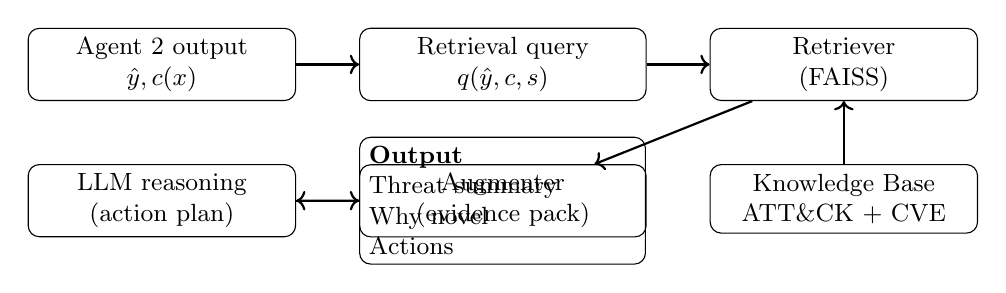
\begin{tikzpicture}[font=\small]
  \node[draw, rounded corners, align=center, minimum width=0.28\columnwidth, minimum height=7mm] (a2out) {Agent 2 output\\$\hat{y}, c(x)$};
  \node[draw, rounded corners, align=center, right=8mm of a2out, minimum width=0.30\columnwidth, minimum height=7mm] (query) {Retrieval query\\$q(\hat{y},c,s)$};
  \node[draw, rounded corners, align=center, right=8mm of query, minimum width=0.28\columnwidth, minimum height=7mm] (retr) {Retriever\\(FAISS)};

  \node[draw, rounded corners, align=center, below=8mm of retr, minimum width=0.28\columnwidth, minimum height=7mm] (kb) {Knowledge Base\\ATT\&CK + CVE};
  \node[draw, rounded corners, align=center, below=8mm of query, minimum width=0.30\columnwidth, minimum height=7mm] (aug) {Augmenter\\(evidence pack)};
  \node[draw, rounded corners, align=center, below=8mm of a2out, minimum width=0.28\columnwidth, minimum height=7mm] (llm) {LLM reasoning\\(action plan)};

  \draw[->, thick] (a2out) -- (query);
  \draw[->, thick] (query) -- (retr);
  \draw[->, thick] (kb) -- (retr);
  \draw[->, thick] (retr) -- (aug);
  \draw[->, thick] (aug) -- (llm);

  \node[draw, rounded corners, align=left, right=8mm of llm, text width=0.28\columnwidth] (out) {\textbf{Output}\\Threat summary\\Why novel\\Actions};
  \draw[->, thick] (llm) -- (out);
\end{tikzpicture}
\caption{Agent 3 RAG pipeline: retrieve evidence then generate structured actions.}
\label{fig:rag_pipeline}
\end{figure}

\subsection{Action Space and Mitigation Mapping}
\label{sec:action_space}

To connect classification outcomes to actionable guidance, we define a compact action space aligned to common NIDS categories and ATT\&CK technique identifiers. The mapping serves two purposes: (i) it provides a consistent schema to evaluate action-plan quality, and (ii) it enables deterministic fallbacks when the LLM cannot be used.

\begin{table}[t]
\caption{Action space mapping from dataset labels to ATT\&CK techniques (representative).}
\label{tab:action_space}
\centering
\begin{tabular}{clll}
\toprule
\textbf{ID} & \textbf{Category} & \textbf{Dataset mapping} & \textbf{MITRE techniques}\\
\midrule
0 & Normal & Normal/Benign & --\\
1 & DoS/DDoS & DoS (UNSW), DoS Hulk (CIC) & T1498, T1499\\
2 & Reconnaissance & Recon (UNSW), PortScan (CIC) & T1046, T1595\\
3 & Exploits & Exploits/Shellcode (UNSW) & T1190, T1059\\
4 & Brute Force & Fuzzers (UNSW) & T1110, T1078\\
5 & Malware & Backdoor/Worms/Generic (UNSW) & T1059, T1071\\
6 & Analysis & Analysis (UNSW), Heartbleed (CIC) & T1040, T1557\\
\bottomrule
\end{tabular}
\end{table}

\subsection{Reproducibility Notes}
\label{sec:reproducibility_notes}

We report all hyperparameters required to reproduce the pipeline, including Agent 1 architecture and $\tau$, Agent 2 hyperparameters and confidence threshold $\gamma$, and Agent 3 retrieval configuration (embedding model, $k$, and KB sources). Since Agent 3 depends on an external LLM endpoint, we fix the prompt template and decoding parameters (temperature, max tokens) and cache retrieved evidence to ensure consistent outputs across reruns. We also log seeds and software versions to reduce variance in reported results \cite{Dodge2019Reporting}.

% -----------------------------
% References for this standalone Methodology section.
% If your main paper uses BibTeX, move these \bibitem entries into your .bib.
\begin{thebibliography}{99}
\bibitem{Moustafa2015UNSW}
N. Moustafa and J. Slay, ``UNSW-NB15: A comprehensive data set for network intrusion detection systems,'' in \emph{Proc. Military Communications and Information Systems Conference (MilCIS)}, 2015.

\bibitem{Moustafa2015UNSW2}
N. Moustafa and J. Slay, ``The evaluation of network anomaly detection systems: Statistical analysis of the UNSW-NB15 data set and the comparison with the KDD99 data set,'' \emph{Information Security Journal: A Global Perspective}, vol. 25, no. 1--3, pp. 18--31, 2016.

\bibitem{Sharafaldin2018CICIDS}
I. Sharafaldin, A. H. Lashkari, and A. A. Ghorbani, ``Toward generating a new intrusion detection dataset and intrusion traffic characterization,'' in \emph{Proc. Int. Conf. Information Systems Security and Privacy (ICISSP)}, 2018.

\bibitem{Hinton2006Reducing}
G. E. Hinton and R. R. Salakhutdinov, ``Reducing the dimensionality of data with neural networks,'' \emph{Science}, vol. 313, no. 5786, pp. 504--507, 2006.

\bibitem{Mirsky2018Kitsune}
Y. Mirsky, T. Doitshman, Y. Elovici, and A. Shabtai, ``Kitsune: An ensemble of autoencoders for online network intrusion detection,'' in \emph{Proc. NDSS}, 2018.

\bibitem{Chen2016XGBoost}
T. Chen and C. Guestrin, ``XGBoost: A scalable tree boosting system,'' in \emph{Proc. ACM SIGKDD}, 2016, pp. 785--794.

\bibitem{Chawla2002SMOTE}
N. V. Chawla, K. W. Bowyer, L. O. Hall, and W. P. Kegelmeyer, ``SMOTE: Synthetic minority over-sampling technique,'' \emph{J. Artif. Intell. Res.}, vol. 16, pp. 321--357, 2002.

\bibitem{Pedregosa2011Scikit}
F. Pedregosa \emph{et al.}, ``Scikit-learn: Machine learning in Python,'' \emph{J. Mach. Learn. Res.}, vol. 12, pp. 2825--2830, 2011.

\bibitem{Scheirer2013OpenSet}
W. J. Scheirer, A. Rocha, R. J. Micheals, and T. E. Boult, ``Toward open set recognition,'' \emph{IEEE Trans. Pattern Anal. Mach. Intell.}, vol. 35, no. 7, pp. 1757--1772, 2013.

\bibitem{Bendale2016OpenMax}
A. Bendale and T. E. Boult, ``Towards open set deep networks,'' in \emph{Proc. CVPR}, 2016.

\bibitem{Lewis2020RAG}
P. Lewis \emph{et al.}, ``Retrieval-augmented generation for knowledge-intensive NLP tasks,'' in \emph{Proc. NeurIPS}, 2020.

\bibitem{Reimers2019SentenceBERT}
N. Reimers and I. Gurevych, ``Sentence-BERT: Sentence embeddings using Siamese BERT-networks,'' in \emph{Proc. EMNLP-IJCNLP}, 2019.

\bibitem{Johnson2019FAISS}
J. Johnson, M. Douze, and H. J\'egou, ``Billion-scale similarity search with GPUs,'' \emph{IEEE Trans. Big Data}, vol. 7, no. 3, pp. 535--547, 2021 (early access 2019).

\bibitem{MITREATTACK}
MITRE, ``MITRE ATT\&CK,'' 2026. [Online]. Available: \url{https://attack.mitre.org/}. Accessed: Apr. 18, 2026.

\bibitem{MITRECVE}
MITRE, ``Common Vulnerabilities and Exposures (CVE),'' 2026. [Online]. Available: \url{https://www.cve.org/}. Accessed: Apr. 18, 2026.

\bibitem{NISTNVD}
National Institute of Standards and Technology, ``National Vulnerability Database (NVD),'' 2026. [Online]. Available: \url{https://nvd.nist.gov/}. Accessed: Apr. 18, 2026.

\bibitem{Dodge2019Reporting}
J. Dodge \emph{et al.}, ``Show your work: Improved reporting of experimental results,'' in \emph{Proc. EMNLP-IJCNLP}, 2019.
\end{thebibliography}
 from an IEEEtran main paper.
% Required packages in main preamble: amsmath, amssymb, graphicx, booktabs, siunitx, tikz.
% TikZ libraries recommended: \usetikzlibrary{positioning,arrows.meta}
% If you compile standalone, wrap this in an IEEEtran document and include the bibliography.

\section{Methodology}
\label{sec:methodology}

We propose a hierarchical, three-agent intrusion detection and response pipeline that balances (i) real-time filtering, (ii) accurate attack-family classification, and (iii) grounded analyst-facing action planning. The design follows a progressive offloading strategy: low-cost models handle the full traffic stream, while expensive reasoning is invoked only for ambiguous or high-risk events. This is aligned with practical intrusion detection deployments, where early-stage filters reduce throughput to downstream analysis stages \cite{Mirsky2018Kitsune}.

\subsection{Data Preparation and Preprocessing}
\label{sec:data_preparation}

This section describes dataset selection, splits, cleaning, feature engineering, and preprocessing. These steps precede the three agents and ensure that all models operate on consistent feature representations.

\subsubsection{Dataset selection and files}
\textbf{Primary benchmark.} We use UNSW-NB15 as the main benchmark dataset for network intrusion detection, due to its diversity of attack types and its structured feature representation \cite{Moustafa2015UNSW,Moustafa2015UNSW2}.

\textbf{Structured train/test splits.} We use the official structured CSV files:
\begin{itemize}
  \item \emph{Training:} \texttt{UNSW\_NB15\_training-set.csv}
  \item \emph{Testing:} \texttt{UNSW\_NB15\_testing-set.csv}
\end{itemize}

\textbf{Raw distribution evaluation.} To approximate ``in-the-wild'' distributions and validate robustness, we additionally evaluate on the raw UNSW-NB15 split files (\texttt{UNSW-NB15\_1.csv} to \texttt{UNSW-NB15\_4.csv}). These files contain the same 49 columns but do not include headers and may differ in column ordering; therefore we load them with an explicit schema to avoid column-mismatch errors.

\subsubsection{Loading, schema alignment, and cleaning}
We implement dataset ingestion using modular components (a \emph{DataLoader} for loading/initial cleaning and a \emph{Preprocessor} for normalization and encoding). This modularity supports reproducibility and simplifies extending to additional datasets.

\textbf{Schema alignment for raw files.} For raw files without headers, we use a dedicated loader that assigns the 49 column names explicitly (47 features plus \texttt{attack\_cat} and \texttt{label}) and normalizes label fields:
\begin{itemize}
  \item Missing or empty \texttt{attack\_cat} values are mapped to \emph{Normal}.
  \item The binary \texttt{label} field is coerced to integer, where 0 indicates normal and 1 indicates attack.
  \item Category strings are stripped and standardized (e.g., minor whitespace variants are normalized).
\end{itemize}

\textbf{Missing values and numeric coercion.} We treat missing values and invalid numeric fields using robust conversions (coerce-to-numeric followed by imputation). In the general preprocessing pipeline, we use simple imputers (median for numeric features and mode for categorical features) to avoid dropping flows and to preserve deployment realism \cite{Pedregosa2011Scikit}.

\subsubsection{Feature engineering}
We compute derived features that improve separability and capture traffic dynamics. In particular, we compute the connection rate:
\begin{equation}
\texttt{rate} = \frac{\texttt{spkts}+\texttt{dpkts}}{\texttt{dur}+\epsilon},
\end{equation}
with $\epsilon>0$ to avoid division by zero. All engineered features are computed deterministically and are included consistently across train/test and raw evaluation.

\subsubsection{Normalization and encoding}
\textbf{Numerical scaling.} We apply min--max scaling to numerical features, matching the default configuration used by the pipeline. Min--max scaling is particularly suitable for autoencoders, where feature ranges can dominate reconstruction loss if left unnormalized. Our implementation uses standard preprocessing utilities (e.g., \texttt{MinMaxScaler}) \cite{Pedregosa2011Scikit}.

\textbf{Categorical encoding.} Categorical columns (e.g., \texttt{proto}, \texttt{service}, \texttt{state}) are encoded either via integer factorization (label encoding) or via one-hot encoding depending on the experiment configuration. In our baseline, we use label encoding to keep the feature dimensionality stable and to simplify deployment.

\subsubsection{Sampling and reproducibility}
To enable fair comparisons across models, we use fixed random seeds (e.g., \texttt{random\_state}=42) for sampling and train/test splits. All preprocessing artifacts (scaler parameters, encoders, and imputers) are fit on the training split and reused unchanged for validation/test transformations, preventing leakage.

\textbf{Class-imbalance handling for supervised training.} UNSW-NB15 exhibits class imbalance (normal traffic dominates, while some attack categories are rare). For Agent~2 training, we apply SMOTE oversampling \emph{only on the training split} after preprocessing to improve minority-class recall while keeping evaluation unbiased \cite{Chawla2002SMOTE}.

\subsection{Pipeline Overview and Decision Flow}
\label{sec:method_overview}

Let $x \in \mathbb{R}^d$ denote a network-flow feature vector extracted from raw packets (e.g., connection statistics, byte/packet counts, TTL/state features, and aggregate temporal features). We follow the feature format provided by standard IDS benchmarks such as UNSW-NB15 \cite{Moustafa2015UNSW}.

The pipeline produces:
\begin{itemize}
  \item a gate decision (Normal vs Anomalous),
  \item a threat category label among known classes, optionally with an ``Unknown/Zero-day'' flag,
  \item a grounded, structured action plan (recommended actions, relevant ATT\&CK techniques, and candidate CVEs when applicable).
\end{itemize}

\textbf{Preprocessing.} For Agents 1 and 2, tabular features are standardized using statistics computed on the training split (mean/variance scaling). Categorical features (if present) are one-hot encoded. The anomaly score produced by Agent 1 is appended to the Agent 2 feature vector to provide a consistent signal of ``distance from normality''.

\textbf{Hierarchical offloading policy.} The system executes:
\begin{enumerate}
  \item \textbf{Agent 1 (Autoencoder gate):} compute anomaly score $s(x)$ and decide $g(x)\in\{\text{Normal},\text{Anomalous}\}$.
  \item \textbf{Agent 2 (XGBoost classifier):} if $g(x)=\text{Anomalous}$, predict class probabilities $p(y\mid x)$ over $K$ known categories and a confidence score $c(x)=\max_y p(y\mid x)$.
  \item \textbf{Agent 3 (RAG+LLM action planner):} if $c(x)<\gamma$ (low confidence) or if Agent 2 explicitly flags ``Unknown/Zero-day'', retrieve threat-intelligence context and generate an action plan.
\end{enumerate}

\textbf{Rationale.} Agent 1 is optimized for high recall and low latency, ensuring that potentially malicious traffic is not missed. Agent 2 provides a low-cost categorical interpretation to support automated response policies for known threats. Agent 3 is invoked selectively to (i) explain uncertain events and (ii) provide grounded response actions using external threat intelligence, reducing hallucinations relative to purely parametric generation \cite{Lewis2020RAG}.

\begin{figure}[t]
\centering
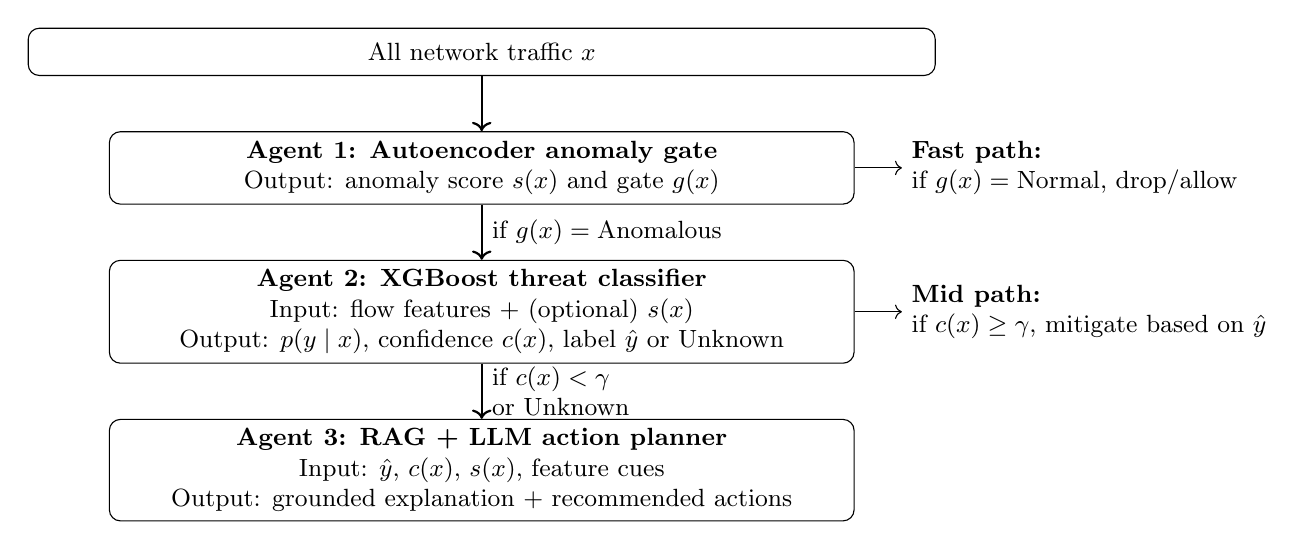
\begin{tikzpicture}[node distance=7mm, font=\small]
  \node[draw, rounded corners, align=center, minimum width=0.95\columnwidth, minimum height=6mm] (traffic) {All network traffic $x$};

  \node[draw, rounded corners, align=center, below=of traffic, minimum width=0.78\columnwidth] (a1) {\textbf{Agent 1: Autoencoder anomaly gate}\\
  Output: anomaly score $s(x)$ and gate $g(x)$};

  \node[draw, rounded corners, align=center, below=of a1, minimum width=0.78\columnwidth] (a2) {\textbf{Agent 2: XGBoost threat classifier}\\
  Input: flow features + (optional) $s(x)$\\
  Output: $p(y\mid x)$, confidence $c(x)$, label $\hat{y}$ or Unknown};

  \node[draw, rounded corners, align=center, below=of a2, minimum width=0.78\columnwidth] (a3) {\textbf{Agent 3: RAG + LLM action planner}\\
  Input: $\hat{y}$, $c(x)$, $s(x)$, feature cues\\
  Output: grounded explanation + recommended actions};

  \draw[->, thick] (traffic) -- (a1);
  \draw[->, thick] (a1) -- node[right, align=left] {if $g(x)=\text{Anomalous}$} (a2);
  \draw[->, thick] (a2) -- node[right, align=left] {if $c(x)<\gamma$\\or Unknown} (a3);

  \node[align=left, right=6mm of a1] (drop) {\textbf{Fast path:}\\if $g(x)=\text{Normal}$, drop/allow};
  \draw[->] (a1.east) -- (drop.west);

  \node[align=left, right=6mm of a2] (mit) {\textbf{Mid path:}\\if $c(x)\ge\gamma$, mitigate based on $\hat{y}$};
  \draw[->] (a2.east) -- (mit.west);
\end{tikzpicture}
\caption{Hierarchical offloading decision flow for the three-agent pipeline.}
\label{fig:hierarchical_offloading}
\end{figure}

\subsection{Agent 1: Autoencoder Anomaly Detector (Gate)}
\label{sec:agent1_method}

\subsubsection{Model architecture}
Agent 1 is a feed-forward PyTorch autoencoder trained to reconstruct benign-dominant traffic. The architecture follows a symmetric bottleneck design (input dimension $d=40$):
\begin{equation}
40 \rightarrow 32 \rightarrow 16 \rightarrow 8 \rightarrow 16 \rightarrow 32 \rightarrow 40,
\end{equation}
where the bottleneck encourages compression into a low-dimensional latent representation. Autoencoders are widely used for anomaly detection by learning normal patterns and flagging reconstruction deviations \cite{Hinton2006Reducing,Mirsky2018Kitsune}.

\textbf{Training objective.} The autoencoder is trained to minimize reconstruction loss on the training split, dominated by Normal traffic:
\begin{equation}
 \min_\theta\; \mathbb{E}_{x\sim\mathcal{D}_{\text{train}}}\left[\lVert x - f_\theta(x)\rVert_2^2\right].
\end{equation}
We use mini-batch optimization (Adam) with early stopping based on validation loss to prevent overfitting.

\subsubsection{Anomaly scoring}
Let $f_\theta(\cdot)$ denote the autoencoder reconstruction function. The anomaly score is computed as the mean squared reconstruction error:
\begin{equation}
 s(x) = \frac{1}{d}\lVert x - f_\theta(x) \rVert_2^2.
\end{equation}
The gate decision is:
\begin{equation}
 g(x) = \mathbb{I}[s(x) \ge \tau],
\end{equation}
where $\tau$ is calibrated on a validation split to achieve a target recall/false-positive trade-off. We select $\tau$ using either (i) a quantile rule on Normal reconstruction errors or (ii) a validation sweep to maximize attack recall at an acceptable false-positive rate.

\textbf{Operating point.} Since the system is designed to avoid missing attacks, we bias $\tau$ toward high recall even if it increases false positives; downstream agents and RAG-based reasoning mitigate the cost by handling only escalated flows.

\subsubsection{Confidence signal}
We additionally expose a normalized confidence proxy derived from the distance to the threshold:
\begin{equation}
 \kappa(x) = \sigma\left(\alpha\,(s(x)-\tau)\right),
\end{equation}
where $\sigma$ is a logistic function and $\alpha$ controls steepness. This scalar is used (i) as an auxiliary feature for Agent 2 to improve separability and (ii) as an escalation cue to Agent 3 when confidence is low.

\subsection{Agent 2: XGBoost Threat Classifier}
\label{sec:agent2_method}

Agent 2 performs supervised multi-class classification over $K=10$ categories (Normal plus nine attack families). We use gradient-boosted decision trees due to their strong performance on tabular intrusion datasets and low inference latency \cite{Chen2016XGBoost}.

\subsubsection{Input features}
For flows flagged anomalous by Agent 1, Agent 2 receives:
\begin{itemize}
  \item raw flow features $x$,
  \item the anomaly score $s(x)$ (or confidence proxy $\kappa(x)$) from Agent 1,
  \item optional engineered statistics (e.g., z-scored feature groups).
\end{itemize}

\textbf{Feature fusion.} The anomaly score acts as a global indicator of deviation from normal behavior and is particularly useful for borderline cases that may be underrepresented in supervised labels.

\subsubsection{Training and imbalance handling}
Class imbalance is addressed using SMOTE oversampling and class-weighted learning, augmented by per-class decision thresholds to balance recall for rare categories \cite{Chawla2002SMOTE}.

Concretely, SMOTE synthesizes minority samples by interpolating between nearest neighbors in feature space. In addition, we apply class weights inversely proportional to class frequency in the loss, and tune per-class decision thresholds on the validation split to improve minority recall without collapsing precision.

We use the following representative hyperparameters (as configured in our implementation): maximum depth $8$, learning rate $0.05$, and $200$ estimators. Early stopping is applied using a validation split.

\subsubsection{Open-set / ``Unknown'' handling (zero-day flag)}
To operationalize zero-day uncertainty, we convert the closed-set classifier into an open-set detector by thresholding confidence:
\begin{equation}
 c(x) = \max_{y\in\{1,\dots,K\}} p(y\mid x).
\end{equation}
If $c(x) < \gamma$ (with $\gamma=0.5$ in our implementation), Agent 2 outputs \emph{Unknown/Zero-day}. This confidence-threshold heuristic is a pragmatic approximation to open-set recognition when explicit unknown-class training is not available; it complements established open-set formulations by explicitly routing uncertain cases to deeper analysis \cite{Scheirer2013OpenSet,Bendale2016OpenMax}.

\textbf{Calibration note.} While boosting models often provide sharp probabilities, confidence thresholds are still sensitive to dataset shift. Therefore, $\gamma$ should be tuned with LOAO-style splits and monitored via false-unknown rate on benign traffic.

\subsection{Agent 3: Retrieval-Augmented Action Planning (RAG+LLM)}
\label{sec:agent3_method}

Agent 3 is invoked only for low-confidence or unknown cases and generates grounded analyst-facing outputs. We adopt Retrieval-Augmented Generation (RAG) to combine parametric LLM reasoning with non-parametric retrieval from a curated knowledge base \cite{Lewis2020RAG}.

\subsubsection{Knowledge sources and representation}
The knowledge base (KB) contains threat intelligence artifacts such as:
\begin{itemize}
  \item MITRE ATT\&CK techniques, tactics, and mitigations \cite{MITREATTACK},
  \item CVE/NVD vulnerability summaries and common exploitation patterns \cite{MITRECVE,NISTNVD},
  \item dataset-specific attack-pattern notes (e.g., UNSW-NB15 and CIC-IDS2017 mappings) \cite{Moustafa2015UNSW,Sharafaldin2018CICIDS}.
\end{itemize}
Each document is embedded into a dense vector space using a sentence embedding model (HuggingFace-style encoders). In our implementation, we use a lightweight sentence-transformer family model to balance retrieval quality and throughput \cite{Reimers2019SentenceBERT}.

\subsubsection{Vector database and retrieval}
We store embeddings in a FAISS vector index for approximate nearest-neighbor retrieval \cite{Johnson2019FAISS}. For a query $q$, the retriever returns top-$k$ documents:
\begin{equation}
 \{d_1,\dots,d_k\} = \operatorname{TopK}(\operatorname{sim}(\phi(q),\phi(d)))
\end{equation}
where $\phi(\cdot)$ maps text to embeddings and $\operatorname{sim}$ is cosine similarity.

\textbf{Retrieval configuration.} We use $k\in\{3,5\}$ depending on prompt budget. Retrieved documents are de-duplicated by (technique ID, CVE ID) to reduce redundancy.

\subsubsection{Retrieval query construction}
The retrieval query is formed from the model outputs and salient feature cues:
\begin{equation}
 q = \{\hat{y},\,c(x),\,s(x),\,\text{feature importance/profile},\,\text{zero-day flag},\,\text{historical scope}\}.
\end{equation}
This structured query is realized as a text prompt that guides the retriever toward relevant technique and vulnerability entries.

\textbf{Why include features?} For ambiguous cases, adding a brief ``feature profile'' (e.g., unusually high packet rate, many half-open connections, abnormal TTL patterns) encourages retrieval of more specific techniques and mitigations, improving actionability.

\subsubsection{Augmentation and generation}
Retrieved evidence is concatenated (with metadata such as technique IDs and severity) and provided to the LLM with instructions to output:
\begin{enumerate}
  \item a concise threat summary,
  \item a ``why novel'' explanation when flagged unknown,
  \item a prioritized \textbf{Recommended Actions} list.
\end{enumerate}
We enforce a structured output format to improve downstream parsing and to support operational use. When the LLM is unavailable, we fall back to deterministic rule-based actions derived from the mapped action space (Table~\ref{tab:action_space}).

\begin{figure}[t]
\centering
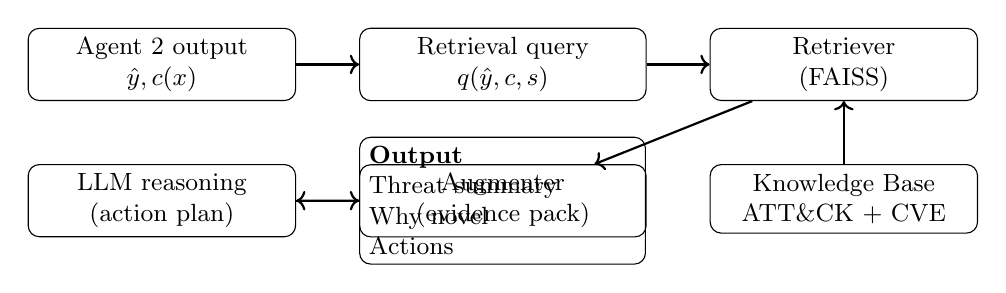
\begin{tikzpicture}[font=\small]
  \node[draw, rounded corners, align=center, minimum width=0.28\columnwidth, minimum height=7mm] (a2out) {Agent 2 output\\$\hat{y}, c(x)$};
  \node[draw, rounded corners, align=center, right=8mm of a2out, minimum width=0.30\columnwidth, minimum height=7mm] (query) {Retrieval query\\$q(\hat{y},c,s)$};
  \node[draw, rounded corners, align=center, right=8mm of query, minimum width=0.28\columnwidth, minimum height=7mm] (retr) {Retriever\\(FAISS)};

  \node[draw, rounded corners, align=center, below=8mm of retr, minimum width=0.28\columnwidth, minimum height=7mm] (kb) {Knowledge Base\\ATT\&CK + CVE};
  \node[draw, rounded corners, align=center, below=8mm of query, minimum width=0.30\columnwidth, minimum height=7mm] (aug) {Augmenter\\(evidence pack)};
  \node[draw, rounded corners, align=center, below=8mm of a2out, minimum width=0.28\columnwidth, minimum height=7mm] (llm) {LLM reasoning\\(action plan)};

  \draw[->, thick] (a2out) -- (query);
  \draw[->, thick] (query) -- (retr);
  \draw[->, thick] (kb) -- (retr);
  \draw[->, thick] (retr) -- (aug);
  \draw[->, thick] (aug) -- (llm);

  \node[draw, rounded corners, align=left, right=8mm of llm, text width=0.28\columnwidth] (out) {\textbf{Output}\\Threat summary\\Why novel\\Actions};
  \draw[->, thick] (llm) -- (out);
\end{tikzpicture}
\caption{Agent 3 RAG pipeline: retrieve evidence then generate structured actions.}
\label{fig:rag_pipeline}
\end{figure}

\subsection{Action Space and Mitigation Mapping}
\label{sec:action_space}

To connect classification outcomes to actionable guidance, we define a compact action space aligned to common NIDS categories and ATT\&CK technique identifiers. The mapping serves two purposes: (i) it provides a consistent schema to evaluate action-plan quality, and (ii) it enables deterministic fallbacks when the LLM cannot be used.

\begin{table}[t]
\caption{Action space mapping from dataset labels to ATT\&CK techniques (representative).}
\label{tab:action_space}
\centering
\begin{tabular}{clll}
\toprule
\textbf{ID} & \textbf{Category} & \textbf{Dataset mapping} & \textbf{MITRE techniques}\\
\midrule
0 & Normal & Normal/Benign & --\\
1 & DoS/DDoS & DoS (UNSW), DoS Hulk (CIC) & T1498, T1499\\
2 & Reconnaissance & Recon (UNSW), PortScan (CIC) & T1046, T1595\\
3 & Exploits & Exploits/Shellcode (UNSW) & T1190, T1059\\
4 & Brute Force & Fuzzers (UNSW) & T1110, T1078\\
5 & Malware & Backdoor/Worms/Generic (UNSW) & T1059, T1071\\
6 & Analysis & Analysis (UNSW), Heartbleed (CIC) & T1040, T1557\\
\bottomrule
\end{tabular}
\end{table}

\subsection{Reproducibility Notes}
\label{sec:reproducibility_notes}

We report all hyperparameters required to reproduce the pipeline, including Agent 1 architecture and $\tau$, Agent 2 hyperparameters and confidence threshold $\gamma$, and Agent 3 retrieval configuration (embedding model, $k$, and KB sources). Since Agent 3 depends on an external LLM endpoint, we fix the prompt template and decoding parameters (temperature, max tokens) and cache retrieved evidence to ensure consistent outputs across reruns. We also log seeds and software versions to reduce variance in reported results \cite{Dodge2019Reporting}.

% -----------------------------
% References for this standalone Methodology section.
% If your main paper uses BibTeX, move these \bibitem entries into your .bib.
\begin{thebibliography}{99}
\bibitem{Moustafa2015UNSW}
N. Moustafa and J. Slay, ``UNSW-NB15: A comprehensive data set for network intrusion detection systems,'' in \emph{Proc. Military Communications and Information Systems Conference (MilCIS)}, 2015.

\bibitem{Moustafa2015UNSW2}
N. Moustafa and J. Slay, ``The evaluation of network anomaly detection systems: Statistical analysis of the UNSW-NB15 data set and the comparison with the KDD99 data set,'' \emph{Information Security Journal: A Global Perspective}, vol. 25, no. 1--3, pp. 18--31, 2016.

\bibitem{Sharafaldin2018CICIDS}
I. Sharafaldin, A. H. Lashkari, and A. A. Ghorbani, ``Toward generating a new intrusion detection dataset and intrusion traffic characterization,'' in \emph{Proc. Int. Conf. Information Systems Security and Privacy (ICISSP)}, 2018.

\bibitem{Hinton2006Reducing}
G. E. Hinton and R. R. Salakhutdinov, ``Reducing the dimensionality of data with neural networks,'' \emph{Science}, vol. 313, no. 5786, pp. 504--507, 2006.

\bibitem{Mirsky2018Kitsune}
Y. Mirsky, T. Doitshman, Y. Elovici, and A. Shabtai, ``Kitsune: An ensemble of autoencoders for online network intrusion detection,'' in \emph{Proc. NDSS}, 2018.

\bibitem{Chen2016XGBoost}
T. Chen and C. Guestrin, ``XGBoost: A scalable tree boosting system,'' in \emph{Proc. ACM SIGKDD}, 2016, pp. 785--794.

\bibitem{Chawla2002SMOTE}
N. V. Chawla, K. W. Bowyer, L. O. Hall, and W. P. Kegelmeyer, ``SMOTE: Synthetic minority over-sampling technique,'' \emph{J. Artif. Intell. Res.}, vol. 16, pp. 321--357, 2002.

\bibitem{Pedregosa2011Scikit}
F. Pedregosa \emph{et al.}, ``Scikit-learn: Machine learning in Python,'' \emph{J. Mach. Learn. Res.}, vol. 12, pp. 2825--2830, 2011.

\bibitem{Scheirer2013OpenSet}
W. J. Scheirer, A. Rocha, R. J. Micheals, and T. E. Boult, ``Toward open set recognition,'' \emph{IEEE Trans. Pattern Anal. Mach. Intell.}, vol. 35, no. 7, pp. 1757--1772, 2013.

\bibitem{Bendale2016OpenMax}
A. Bendale and T. E. Boult, ``Towards open set deep networks,'' in \emph{Proc. CVPR}, 2016.

\bibitem{Lewis2020RAG}
P. Lewis \emph{et al.}, ``Retrieval-augmented generation for knowledge-intensive NLP tasks,'' in \emph{Proc. NeurIPS}, 2020.

\bibitem{Reimers2019SentenceBERT}
N. Reimers and I. Gurevych, ``Sentence-BERT: Sentence embeddings using Siamese BERT-networks,'' in \emph{Proc. EMNLP-IJCNLP}, 2019.

\bibitem{Johnson2019FAISS}
J. Johnson, M. Douze, and H. J\'egou, ``Billion-scale similarity search with GPUs,'' \emph{IEEE Trans. Big Data}, vol. 7, no. 3, pp. 535--547, 2021 (early access 2019).

\bibitem{MITREATTACK}
MITRE, ``MITRE ATT\&CK,'' 2026. [Online]. Available: \url{https://attack.mitre.org/}. Accessed: Apr. 18, 2026.

\bibitem{MITRECVE}
MITRE, ``Common Vulnerabilities and Exposures (CVE),'' 2026. [Online]. Available: \url{https://www.cve.org/}. Accessed: Apr. 18, 2026.

\bibitem{NISTNVD}
National Institute of Standards and Technology, ``National Vulnerability Database (NVD),'' 2026. [Online]. Available: \url{https://nvd.nist.gov/}. Accessed: Apr. 18, 2026.

\bibitem{Dodge2019Reporting}
J. Dodge \emph{et al.}, ``Show your work: Improved reporting of experimental results,'' in \emph{Proc. EMNLP-IJCNLP}, 2019.
\end{thebibliography}
 from an IEEEtran main paper.
% Required packages in main preamble: amsmath, amssymb, graphicx, booktabs, siunitx, tikz.
% TikZ libraries recommended: \usetikzlibrary{positioning,arrows.meta}
% If you compile standalone, wrap this in an IEEEtran document and include the bibliography.

\section{Methodology}
\label{sec:methodology}

We propose a hierarchical, three-agent intrusion detection and response pipeline that balances (i) real-time filtering, (ii) accurate attack-family classification, and (iii) grounded analyst-facing action planning. The design follows a progressive offloading strategy: low-cost models handle the full traffic stream, while expensive reasoning is invoked only for ambiguous or high-risk events. This is aligned with practical intrusion detection deployments, where early-stage filters reduce throughput to downstream analysis stages \cite{Mirsky2018Kitsune}.

\subsection{Data Preparation and Preprocessing}
\label{sec:data_preparation}

This section describes dataset selection, splits, cleaning, feature engineering, and preprocessing. These steps precede the three agents and ensure that all models operate on consistent feature representations.

\subsubsection{Dataset selection and files}
\textbf{Primary benchmark.} We use UNSW-NB15 as the main benchmark dataset for network intrusion detection, due to its diversity of attack types and its structured feature representation \cite{Moustafa2015UNSW,Moustafa2015UNSW2}.

\textbf{Structured train/test splits.} We use the official structured CSV files:
\begin{itemize}
  \item \emph{Training:} \texttt{UNSW\_NB15\_training-set.csv}
  \item \emph{Testing:} \texttt{UNSW\_NB15\_testing-set.csv}
\end{itemize}

\textbf{Raw distribution evaluation.} To approximate ``in-the-wild'' distributions and validate robustness, we additionally evaluate on the raw UNSW-NB15 split files (\texttt{UNSW-NB15\_1.csv} to \texttt{UNSW-NB15\_4.csv}). These files contain the same 49 columns but do not include headers and may differ in column ordering; therefore we load them with an explicit schema to avoid column-mismatch errors.

\subsubsection{Loading, schema alignment, and cleaning}
We implement dataset ingestion using modular components (a \emph{DataLoader} for loading/initial cleaning and a \emph{Preprocessor} for normalization and encoding). This modularity supports reproducibility and simplifies extending to additional datasets.

\textbf{Schema alignment for raw files.} For raw files without headers, we use a dedicated loader that assigns the 49 column names explicitly (47 features plus \texttt{attack\_cat} and \texttt{label}) and normalizes label fields:
\begin{itemize}
  \item Missing or empty \texttt{attack\_cat} values are mapped to \emph{Normal}.
  \item The binary \texttt{label} field is coerced to integer, where 0 indicates normal and 1 indicates attack.
  \item Category strings are stripped and standardized (e.g., minor whitespace variants are normalized).
\end{itemize}

\textbf{Missing values and numeric coercion.} We treat missing values and invalid numeric fields using robust conversions (coerce-to-numeric followed by imputation). In the general preprocessing pipeline, we use simple imputers (median for numeric features and mode for categorical features) to avoid dropping flows and to preserve deployment realism \cite{Pedregosa2011Scikit}.

\subsubsection{Feature engineering}
We compute derived features that improve separability and capture traffic dynamics. In particular, we compute the connection rate:
\begin{equation}
\texttt{rate} = \frac{\texttt{spkts}+\texttt{dpkts}}{\texttt{dur}+\epsilon},
\end{equation}
with $\epsilon>0$ to avoid division by zero. All engineered features are computed deterministically and are included consistently across train/test and raw evaluation.

\subsubsection{Normalization and encoding}
\textbf{Numerical scaling.} We apply min--max scaling to numerical features, matching the default configuration used by the pipeline. Min--max scaling is particularly suitable for autoencoders, where feature ranges can dominate reconstruction loss if left unnormalized. Our implementation uses standard preprocessing utilities (e.g., \texttt{MinMaxScaler}) \cite{Pedregosa2011Scikit}.

\textbf{Categorical encoding.} Categorical columns (e.g., \texttt{proto}, \texttt{service}, \texttt{state}) are encoded either via integer factorization (label encoding) or via one-hot encoding depending on the experiment configuration. In our baseline, we use label encoding to keep the feature dimensionality stable and to simplify deployment.

\subsubsection{Sampling and reproducibility}
To enable fair comparisons across models, we use fixed random seeds (e.g., \texttt{random\_state}=42) for sampling and train/test splits. All preprocessing artifacts (scaler parameters, encoders, and imputers) are fit on the training split and reused unchanged for validation/test transformations, preventing leakage.

\textbf{Class-imbalance handling for supervised training.} UNSW-NB15 exhibits class imbalance (normal traffic dominates, while some attack categories are rare). For Agent~2 training, we apply SMOTE oversampling \emph{only on the training split} after preprocessing to improve minority-class recall while keeping evaluation unbiased \cite{Chawla2002SMOTE}.

\subsection{Pipeline Overview and Decision Flow}
\label{sec:method_overview}

Let $x \in \mathbb{R}^d$ denote a network-flow feature vector extracted from raw packets (e.g., connection statistics, byte/packet counts, TTL/state features, and aggregate temporal features). We follow the feature format provided by standard IDS benchmarks such as UNSW-NB15 \cite{Moustafa2015UNSW}.

The pipeline produces:
\begin{itemize}
  \item a gate decision (Normal vs Anomalous),
  \item a threat category label among known classes, optionally with an ``Unknown/Zero-day'' flag,
  \item a grounded, structured action plan (recommended actions, relevant ATT\&CK techniques, and candidate CVEs when applicable).
\end{itemize}

\textbf{Preprocessing.} For Agents 1 and 2, tabular features are standardized using statistics computed on the training split (mean/variance scaling). Categorical features (if present) are one-hot encoded. The anomaly score produced by Agent 1 is appended to the Agent 2 feature vector to provide a consistent signal of ``distance from normality''.

\textbf{Hierarchical offloading policy.} The system executes:
\begin{enumerate}
  \item \textbf{Agent 1 (Autoencoder gate):} compute anomaly score $s(x)$ and decide $g(x)\in\{\text{Normal},\text{Anomalous}\}$.
  \item \textbf{Agent 2 (XGBoost classifier):} if $g(x)=\text{Anomalous}$, predict class probabilities $p(y\mid x)$ over $K$ known categories and a confidence score $c(x)=\max_y p(y\mid x)$.
  \item \textbf{Agent 3 (RAG+LLM action planner):} if $c(x)<\gamma$ (low confidence) or if Agent 2 explicitly flags ``Unknown/Zero-day'', retrieve threat-intelligence context and generate an action plan.
\end{enumerate}

\textbf{Rationale.} Agent 1 is optimized for high recall and low latency, ensuring that potentially malicious traffic is not missed. Agent 2 provides a low-cost categorical interpretation to support automated response policies for known threats. Agent 3 is invoked selectively to (i) explain uncertain events and (ii) provide grounded response actions using external threat intelligence, reducing hallucinations relative to purely parametric generation \cite{Lewis2020RAG}.

\begin{figure}[t]
\centering
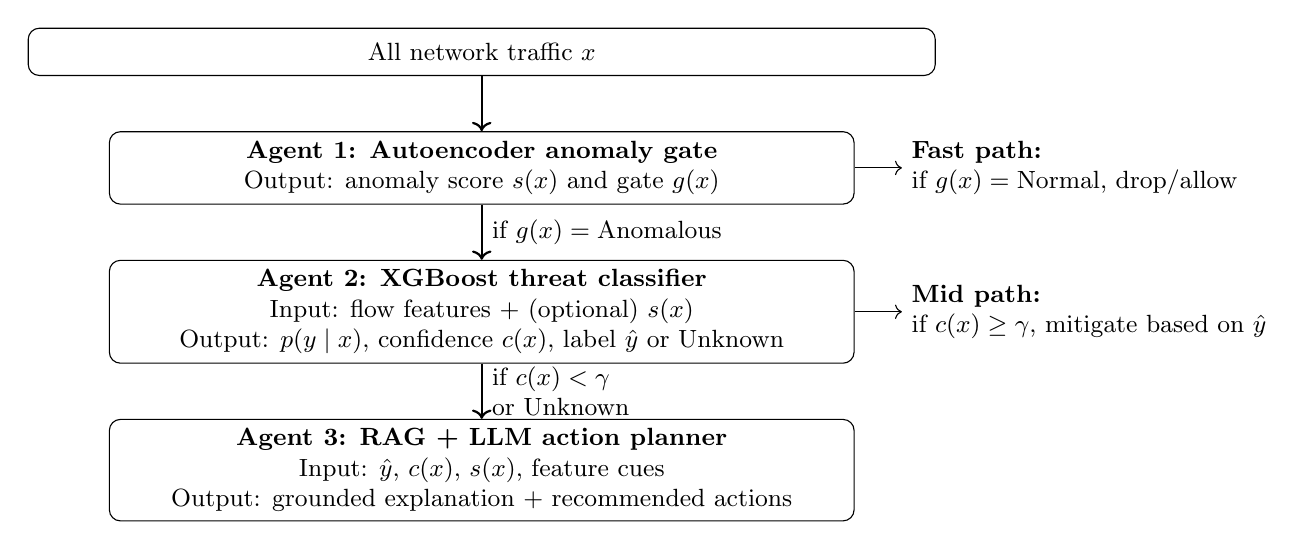
\begin{tikzpicture}[node distance=7mm, font=\small]
  \node[draw, rounded corners, align=center, minimum width=0.95\columnwidth, minimum height=6mm] (traffic) {All network traffic $x$};

  \node[draw, rounded corners, align=center, below=of traffic, minimum width=0.78\columnwidth] (a1) {\textbf{Agent 1: Autoencoder anomaly gate}\\
  Output: anomaly score $s(x)$ and gate $g(x)$};

  \node[draw, rounded corners, align=center, below=of a1, minimum width=0.78\columnwidth] (a2) {\textbf{Agent 2: XGBoost threat classifier}\\
  Input: flow features + (optional) $s(x)$\\
  Output: $p(y\mid x)$, confidence $c(x)$, label $\hat{y}$ or Unknown};

  \node[draw, rounded corners, align=center, below=of a2, minimum width=0.78\columnwidth] (a3) {\textbf{Agent 3: RAG + LLM action planner}\\
  Input: $\hat{y}$, $c(x)$, $s(x)$, feature cues\\
  Output: grounded explanation + recommended actions};

  \draw[->, thick] (traffic) -- (a1);
  \draw[->, thick] (a1) -- node[right, align=left] {if $g(x)=\text{Anomalous}$} (a2);
  \draw[->, thick] (a2) -- node[right, align=left] {if $c(x)<\gamma$\\or Unknown} (a3);

  \node[align=left, right=6mm of a1] (drop) {\textbf{Fast path:}\\if $g(x)=\text{Normal}$, drop/allow};
  \draw[->] (a1.east) -- (drop.west);

  \node[align=left, right=6mm of a2] (mit) {\textbf{Mid path:}\\if $c(x)\ge\gamma$, mitigate based on $\hat{y}$};
  \draw[->] (a2.east) -- (mit.west);
\end{tikzpicture}
\caption{Hierarchical offloading decision flow for the three-agent pipeline.}
\label{fig:hierarchical_offloading}
\end{figure}

\subsection{Agent 1: Autoencoder Anomaly Detector (Gate)}
\label{sec:agent1_method}

\subsubsection{Model architecture}
Agent 1 is a feed-forward PyTorch autoencoder trained to reconstruct benign-dominant traffic. The architecture follows a symmetric bottleneck design (input dimension $d=40$):
\begin{equation}
40 \rightarrow 32 \rightarrow 16 \rightarrow 8 \rightarrow 16 \rightarrow 32 \rightarrow 40,
\end{equation}
where the bottleneck encourages compression into a low-dimensional latent representation. Autoencoders are widely used for anomaly detection by learning normal patterns and flagging reconstruction deviations \cite{Hinton2006Reducing,Mirsky2018Kitsune}.

\textbf{Training objective.} The autoencoder is trained to minimize reconstruction loss on the training split, dominated by Normal traffic:
\begin{equation}
 \min_\theta\; \mathbb{E}_{x\sim\mathcal{D}_{\text{train}}}\left[\lVert x - f_\theta(x)\rVert_2^2\right].
\end{equation}
We use mini-batch optimization (Adam) with early stopping based on validation loss to prevent overfitting.

\subsubsection{Anomaly scoring}
Let $f_\theta(\cdot)$ denote the autoencoder reconstruction function. The anomaly score is computed as the mean squared reconstruction error:
\begin{equation}
 s(x) = \frac{1}{d}\lVert x - f_\theta(x) \rVert_2^2.
\end{equation}
The gate decision is:
\begin{equation}
 g(x) = \mathbb{I}[s(x) \ge \tau],
\end{equation}
where $\tau$ is calibrated on a validation split to achieve a target recall/false-positive trade-off. We select $\tau$ using either (i) a quantile rule on Normal reconstruction errors or (ii) a validation sweep to maximize attack recall at an acceptable false-positive rate.

\textbf{Operating point.} Since the system is designed to avoid missing attacks, we bias $\tau$ toward high recall even if it increases false positives; downstream agents and RAG-based reasoning mitigate the cost by handling only escalated flows.

\subsubsection{Confidence signal}
We additionally expose a normalized confidence proxy derived from the distance to the threshold:
\begin{equation}
 \kappa(x) = \sigma\left(\alpha\,(s(x)-\tau)\right),
\end{equation}
where $\sigma$ is a logistic function and $\alpha$ controls steepness. This scalar is used (i) as an auxiliary feature for Agent 2 to improve separability and (ii) as an escalation cue to Agent 3 when confidence is low.

\subsection{Agent 2: XGBoost Threat Classifier}
\label{sec:agent2_method}

Agent 2 performs supervised multi-class classification over $K=10$ categories (Normal plus nine attack families). We use gradient-boosted decision trees due to their strong performance on tabular intrusion datasets and low inference latency \cite{Chen2016XGBoost}.

\subsubsection{Input features}
For flows flagged anomalous by Agent 1, Agent 2 receives:
\begin{itemize}
  \item raw flow features $x$,
  \item the anomaly score $s(x)$ (or confidence proxy $\kappa(x)$) from Agent 1,
  \item optional engineered statistics (e.g., z-scored feature groups).
\end{itemize}

\textbf{Feature fusion.} The anomaly score acts as a global indicator of deviation from normal behavior and is particularly useful for borderline cases that may be underrepresented in supervised labels.

\subsubsection{Training and imbalance handling}
Class imbalance is addressed using SMOTE oversampling and class-weighted learning, augmented by per-class decision thresholds to balance recall for rare categories \cite{Chawla2002SMOTE}.

Concretely, SMOTE synthesizes minority samples by interpolating between nearest neighbors in feature space. In addition, we apply class weights inversely proportional to class frequency in the loss, and tune per-class decision thresholds on the validation split to improve minority recall without collapsing precision.

We use the following representative hyperparameters (as configured in our implementation): maximum depth $8$, learning rate $0.05$, and $200$ estimators. Early stopping is applied using a validation split.

\subsubsection{Open-set / ``Unknown'' handling (zero-day flag)}
To operationalize zero-day uncertainty, we convert the closed-set classifier into an open-set detector by thresholding confidence:
\begin{equation}
 c(x) = \max_{y\in\{1,\dots,K\}} p(y\mid x).
\end{equation}
If $c(x) < \gamma$ (with $\gamma=0.5$ in our implementation), Agent 2 outputs \emph{Unknown/Zero-day}. This confidence-threshold heuristic is a pragmatic approximation to open-set recognition when explicit unknown-class training is not available; it complements established open-set formulations by explicitly routing uncertain cases to deeper analysis \cite{Scheirer2013OpenSet,Bendale2016OpenMax}.

\textbf{Calibration note.} While boosting models often provide sharp probabilities, confidence thresholds are still sensitive to dataset shift. Therefore, $\gamma$ should be tuned with LOAO-style splits and monitored via false-unknown rate on benign traffic.

\subsection{Agent 3: Retrieval-Augmented Action Planning (RAG+LLM)}
\label{sec:agent3_method}

Agent 3 is invoked only for low-confidence or unknown cases and generates grounded analyst-facing outputs. We adopt Retrieval-Augmented Generation (RAG) to combine parametric LLM reasoning with non-parametric retrieval from a curated knowledge base \cite{Lewis2020RAG}.

\subsubsection{Knowledge sources and representation}
The knowledge base (KB) contains threat intelligence artifacts such as:
\begin{itemize}
  \item MITRE ATT\&CK techniques, tactics, and mitigations \cite{MITREATTACK},
  \item CVE/NVD vulnerability summaries and common exploitation patterns \cite{MITRECVE,NISTNVD},
  \item dataset-specific attack-pattern notes (e.g., UNSW-NB15 and CIC-IDS2017 mappings) \cite{Moustafa2015UNSW,Sharafaldin2018CICIDS}.
\end{itemize}
Each document is embedded into a dense vector space using a sentence embedding model (HuggingFace-style encoders). In our implementation, we use a lightweight sentence-transformer family model to balance retrieval quality and throughput \cite{Reimers2019SentenceBERT}.

\subsubsection{Vector database and retrieval}
We store embeddings in a FAISS vector index for approximate nearest-neighbor retrieval \cite{Johnson2019FAISS}. For a query $q$, the retriever returns top-$k$ documents:
\begin{equation}
 \{d_1,\dots,d_k\} = \operatorname{TopK}(\operatorname{sim}(\phi(q),\phi(d)))
\end{equation}
where $\phi(\cdot)$ maps text to embeddings and $\operatorname{sim}$ is cosine similarity.

\textbf{Retrieval configuration.} We use $k\in\{3,5\}$ depending on prompt budget. Retrieved documents are de-duplicated by (technique ID, CVE ID) to reduce redundancy.

\subsubsection{Retrieval query construction}
The retrieval query is formed from the model outputs and salient feature cues:
\begin{equation}
 q = \{\hat{y},\,c(x),\,s(x),\,\text{feature importance/profile},\,\text{zero-day flag},\,\text{historical scope}\}.
\end{equation}
This structured query is realized as a text prompt that guides the retriever toward relevant technique and vulnerability entries.

\textbf{Why include features?} For ambiguous cases, adding a brief ``feature profile'' (e.g., unusually high packet rate, many half-open connections, abnormal TTL patterns) encourages retrieval of more specific techniques and mitigations, improving actionability.

\subsubsection{Augmentation and generation}
Retrieved evidence is concatenated (with metadata such as technique IDs and severity) and provided to the LLM with instructions to output:
\begin{enumerate}
  \item a concise threat summary,
  \item a ``why novel'' explanation when flagged unknown,
  \item a prioritized \textbf{Recommended Actions} list.
\end{enumerate}
We enforce a structured output format to improve downstream parsing and to support operational use. When the LLM is unavailable, we fall back to deterministic rule-based actions derived from the mapped action space (Table~\ref{tab:action_space}).

\begin{figure}[t]
\centering
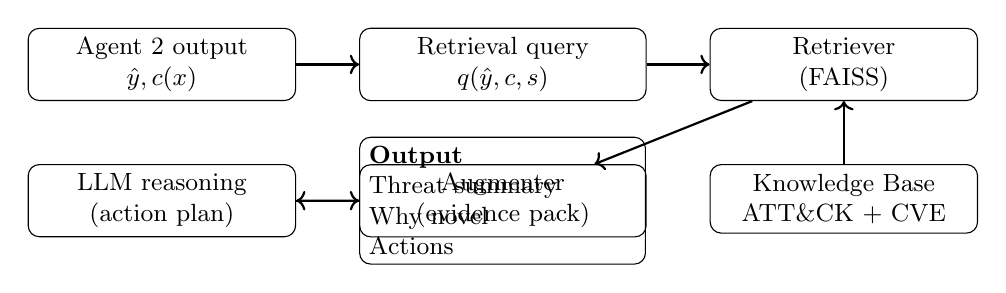
\begin{tikzpicture}[font=\small]
  \node[draw, rounded corners, align=center, minimum width=0.28\columnwidth, minimum height=7mm] (a2out) {Agent 2 output\\$\hat{y}, c(x)$};
  \node[draw, rounded corners, align=center, right=8mm of a2out, minimum width=0.30\columnwidth, minimum height=7mm] (query) {Retrieval query\\$q(\hat{y},c,s)$};
  \node[draw, rounded corners, align=center, right=8mm of query, minimum width=0.28\columnwidth, minimum height=7mm] (retr) {Retriever\\(FAISS)};

  \node[draw, rounded corners, align=center, below=8mm of retr, minimum width=0.28\columnwidth, minimum height=7mm] (kb) {Knowledge Base\\ATT\&CK + CVE};
  \node[draw, rounded corners, align=center, below=8mm of query, minimum width=0.30\columnwidth, minimum height=7mm] (aug) {Augmenter\\(evidence pack)};
  \node[draw, rounded corners, align=center, below=8mm of a2out, minimum width=0.28\columnwidth, minimum height=7mm] (llm) {LLM reasoning\\(action plan)};

  \draw[->, thick] (a2out) -- (query);
  \draw[->, thick] (query) -- (retr);
  \draw[->, thick] (kb) -- (retr);
  \draw[->, thick] (retr) -- (aug);
  \draw[->, thick] (aug) -- (llm);

  \node[draw, rounded corners, align=left, right=8mm of llm, text width=0.28\columnwidth] (out) {\textbf{Output}\\Threat summary\\Why novel\\Actions};
  \draw[->, thick] (llm) -- (out);
\end{tikzpicture}
\caption{Agent 3 RAG pipeline: retrieve evidence then generate structured actions.}
\label{fig:rag_pipeline}
\end{figure}

\subsection{Action Space and Mitigation Mapping}
\label{sec:action_space}

To connect classification outcomes to actionable guidance, we define a compact action space aligned to common NIDS categories and ATT\&CK technique identifiers. The mapping serves two purposes: (i) it provides a consistent schema to evaluate action-plan quality, and (ii) it enables deterministic fallbacks when the LLM cannot be used.

\begin{table}[t]
\caption{Action space mapping from dataset labels to ATT\&CK techniques (representative).}
\label{tab:action_space}
\centering
\begin{tabular}{clll}
\toprule
\textbf{ID} & \textbf{Category} & \textbf{Dataset mapping} & \textbf{MITRE techniques}\\
\midrule
0 & Normal & Normal/Benign & --\\
1 & DoS/DDoS & DoS (UNSW), DoS Hulk (CIC) & T1498, T1499\\
2 & Reconnaissance & Recon (UNSW), PortScan (CIC) & T1046, T1595\\
3 & Exploits & Exploits/Shellcode (UNSW) & T1190, T1059\\
4 & Brute Force & Fuzzers (UNSW) & T1110, T1078\\
5 & Malware & Backdoor/Worms/Generic (UNSW) & T1059, T1071\\
6 & Analysis & Analysis (UNSW), Heartbleed (CIC) & T1040, T1557\\
\bottomrule
\end{tabular}
\end{table}

\subsection{Reproducibility Notes}
\label{sec:reproducibility_notes}

We report all hyperparameters required to reproduce the pipeline, including Agent 1 architecture and $\tau$, Agent 2 hyperparameters and confidence threshold $\gamma$, and Agent 3 retrieval configuration (embedding model, $k$, and KB sources). Since Agent 3 depends on an external LLM endpoint, we fix the prompt template and decoding parameters (temperature, max tokens) and cache retrieved evidence to ensure consistent outputs across reruns. We also log seeds and software versions to reduce variance in reported results \cite{Dodge2019Reporting}.

% -----------------------------
% References for this standalone Methodology section.
% If your main paper uses BibTeX, move these \bibitem entries into your .bib.
\begin{thebibliography}{99}
\bibitem{Moustafa2015UNSW}
N. Moustafa and J. Slay, ``UNSW-NB15: A comprehensive data set for network intrusion detection systems,'' in \emph{Proc. Military Communications and Information Systems Conference (MilCIS)}, 2015.

\bibitem{Moustafa2015UNSW2}
N. Moustafa and J. Slay, ``The evaluation of network anomaly detection systems: Statistical analysis of the UNSW-NB15 data set and the comparison with the KDD99 data set,'' \emph{Information Security Journal: A Global Perspective}, vol. 25, no. 1--3, pp. 18--31, 2016.

\bibitem{Sharafaldin2018CICIDS}
I. Sharafaldin, A. H. Lashkari, and A. A. Ghorbani, ``Toward generating a new intrusion detection dataset and intrusion traffic characterization,'' in \emph{Proc. Int. Conf. Information Systems Security and Privacy (ICISSP)}, 2018.

\bibitem{Hinton2006Reducing}
G. E. Hinton and R. R. Salakhutdinov, ``Reducing the dimensionality of data with neural networks,'' \emph{Science}, vol. 313, no. 5786, pp. 504--507, 2006.

\bibitem{Mirsky2018Kitsune}
Y. Mirsky, T. Doitshman, Y. Elovici, and A. Shabtai, ``Kitsune: An ensemble of autoencoders for online network intrusion detection,'' in \emph{Proc. NDSS}, 2018.

\bibitem{Chen2016XGBoost}
T. Chen and C. Guestrin, ``XGBoost: A scalable tree boosting system,'' in \emph{Proc. ACM SIGKDD}, 2016, pp. 785--794.

\bibitem{Chawla2002SMOTE}
N. V. Chawla, K. W. Bowyer, L. O. Hall, and W. P. Kegelmeyer, ``SMOTE: Synthetic minority over-sampling technique,'' \emph{J. Artif. Intell. Res.}, vol. 16, pp. 321--357, 2002.

\bibitem{Pedregosa2011Scikit}
F. Pedregosa \emph{et al.}, ``Scikit-learn: Machine learning in Python,'' \emph{J. Mach. Learn. Res.}, vol. 12, pp. 2825--2830, 2011.

\bibitem{Scheirer2013OpenSet}
W. J. Scheirer, A. Rocha, R. J. Micheals, and T. E. Boult, ``Toward open set recognition,'' \emph{IEEE Trans. Pattern Anal. Mach. Intell.}, vol. 35, no. 7, pp. 1757--1772, 2013.

\bibitem{Bendale2016OpenMax}
A. Bendale and T. E. Boult, ``Towards open set deep networks,'' in \emph{Proc. CVPR}, 2016.

\bibitem{Lewis2020RAG}
P. Lewis \emph{et al.}, ``Retrieval-augmented generation for knowledge-intensive NLP tasks,'' in \emph{Proc. NeurIPS}, 2020.

\bibitem{Reimers2019SentenceBERT}
N. Reimers and I. Gurevych, ``Sentence-BERT: Sentence embeddings using Siamese BERT-networks,'' in \emph{Proc. EMNLP-IJCNLP}, 2019.

\bibitem{Johnson2019FAISS}
J. Johnson, M. Douze, and H. J\'egou, ``Billion-scale similarity search with GPUs,'' \emph{IEEE Trans. Big Data}, vol. 7, no. 3, pp. 535--547, 2021 (early access 2019).

\bibitem{MITREATTACK}
MITRE, ``MITRE ATT\&CK,'' 2026. [Online]. Available: \url{https://attack.mitre.org/}. Accessed: Apr. 18, 2026.

\bibitem{MITRECVE}
MITRE, ``Common Vulnerabilities and Exposures (CVE),'' 2026. [Online]. Available: \url{https://www.cve.org/}. Accessed: Apr. 18, 2026.

\bibitem{NISTNVD}
National Institute of Standards and Technology, ``National Vulnerability Database (NVD),'' 2026. [Online]. Available: \url{https://nvd.nist.gov/}. Accessed: Apr. 18, 2026.

\bibitem{Dodge2019Reporting}
J. Dodge \emph{et al.}, ``Show your work: Improved reporting of experimental results,'' in \emph{Proc. EMNLP-IJCNLP}, 2019.
\end{thebibliography}


\section*{Acknowledgment}
Placeholder.

\begin{thebibliography}{99}
\bibitem{mcmahan2017fedavg}
B.~McMahan, E.~Moore, D.~Ramage, S.~Hampson, and B.~A. y~Arcas, ``Communication-Efficient Learning of Deep Networks from Decentralized Data,'' in \emph{Proc. AISTATS}, 2017.

\bibitem{kairouz2021flsurvey}
P.~Kairouz \emph{et al.}, ``Advances and Open Problems in Federated Learning,'' \emph{Foundations and Trends in Machine Learning}, vol.~14, no.~1--2, pp.~1--210, 2021.

\bibitem{beutel2020flower}
D.~Beutel \emph{et al.}, ``Flower: A Friendly Federated Learning Research Framework,'' \emph{arXiv preprint arXiv:2007.14390}, 2020.

\bibitem{dwork2006dp}
C.~Dwork, ``Differential Privacy,'' in \emph{Proc. ICALP}, 2006.

\bibitem{abadi2016dpsgd}
M.~Abadi \emph{et al.}, ``Deep Learning with Differential Privacy,'' in \emph{Proc. ACM CCS}, 2016.

\bibitem{blanchard2017byzantine}
P.~Blanchard, R.~Guerraoui, J.~Stainer, ``Machine Learning with Adversaries: Byzantine Tolerant Gradient Descent,'' in \emph{Proc. NeurIPS}, 2017.

\bibitem{moustafa2015unsw}
N.~Moustafa and J.~Slay, ``UNSW-NB15: A Comprehensive Data Set for Network Intrusion Detection Systems,'' in \emph{Proc. MilCIS}, 2015.

\bibitem{xgboost2016}
T.~Chen and C.~Guestrin, ``XGBoost: A Scalable Tree Boosting System,'' in \emph{Proc. ACM SIGKDD}, 2016.

\bibitem{scheirer2013openset}
W.~J. Scheirer, A.~Rocha, A.~Sapkota, and T.~E. Boult, ``Toward Open Set Recognition,'' \emph{IEEE Transactions on Pattern Analysis and Machine Intelligence}, vol.~35, no.~7, pp.~1757--1772, 2013.

\bibitem{bendale2016openset}
A.~Bendale and T.~Boult, ``Towards Open Set Deep Networks,'' in \emph{Proc. CVPR}, 2016.

\bibitem{sakurada2014ae}
M.~Sakurada and T.~Yairi, ``Anomaly Detection Using Autoencoders with Nonlinear Dimensionality Reduction,'' in \emph{Proc. MLSDA}, 2014.

\bibitem{chalapathy2019anomaly}
R.~Chalapathy and S.~Chawla, ``Deep Learning for Anomaly Detection: A Survey,'' \emph{arXiv preprint arXiv:1901.03407}, 2019.

\bibitem{goodfellow2016dl}
I.~Goodfellow, Y.~Bengio, and A.~Courville, \emph{Deep Learning}. MIT Press, 2016.

\bibitem{lewis2020rag}
P.~Lewis \emph{et al.}, ``Retrieval-Augmented Generation for Knowledge-Intensive NLP Tasks,'' in \emph{Proc. NeurIPS}, 2020.

\bibitem{nist80061}
K.~Scarfone, P.~Mell, A.~Souppaya, and M.~Olsen, ``Computer Security Incident Handling Guide,'' NIST Special Publication 800-61 Revision 2, 2012.

\bibitem{attck}
MITRE, ``MITRE ATT\&CK,'' \url{https://attack.mitre.org/}, accessed 2026-04-17.

\bibitem{cve}
MITRE, ``Common Vulnerabilities and Exposures (CVE),'' \url{https://www.cve.org/}, accessed 2026-04-17.

\end{thebibliography}

% Optional: when you're ready to include results, uncomment and add packages above.
% % Results Section (copy-paste ready)
% Intended to be \input{}-ed from an IEEEtran main paper.
% Requires packages: booktabs, multirow, siunitx, pgfplots, pgfplotstable

% -----------------------------
\section{Results}
\label{sec:results}

We report results for the three-agent pipeline on UNSW-NB15-style IDS categories \cite{moustafa2015unsw}: Agent~1 (autoencoder anomaly gate), Agent~2 (XGBoost classifier with an ``Unknown/Zero-day'' option), and Agent~3 (RAG+LLM action planning grounded in MITRE ATT\&CK / CVE context) \cite{chen2016xgboost,lewis2020rag,mitreattack}.

\subsection{Experimental Protocol}
\label{sec:protocol}

\textbf{Dataset and labels.} We use UNSW-NB15 attack categories (e.g., \emph{DoS}, \emph{Exploits}, \emph{Reconnaissance}, \emph{Backdoor}, \emph{Fuzzers}, \emph{Shellcode}, \emph{Worms}) plus \emph{Normal} traffic \cite{moustafa2015unsw}. Agent~1 is evaluated as a binary gate (Normal vs Attack). Agent~2 is evaluated as a multi-class classifier on known categories.

\textbf{Zero-day definition: LOAO.} We define ``zero-day'' with a \emph{Left-One-Attack-Out (LOAO)} protocol. Each organization/client trains on a filtered local dataset that excludes one attack family; that excluded family becomes the client’s ``never-seen'' (zero-day) pattern at test time.

\textbf{LOAO configuration.} We use three clients:
\begin{itemize}
  \item Client A holds out \textbf{DoS} ($z_A=\text{DoS}$),
  \item Client B holds out \textbf{Exploits} ($z_B=\text{Exploits}$),
  \item Client C holds out \textbf{Reconnaissance} ($z_C=\text{Reconnaissance}$).
\end{itemize}

\textbf{Federated setup (Agent~1 only).} We run $R=10$ federated rounds with FedAvg \cite{mcmahan2017fedavg}, three clients participating each round, and one local epoch per round. We report per-round client validation accuracy (overall framework accuracy after gating) and show that clients converge toward a shared global model.

\subsection{Main Quantitative Results}
\label{sec:main-results}

\subsubsection{Agent~1 anomaly detection (autoencoder gate)}
Agent~1 separates benign and malicious flows using reconstruction error. Following the operating point selected in our implementation slides, we set the decision threshold to $\tau=0.0712$ and obtain high attack recall while maintaining low per-flow latency on CPU.

\begin{table}[t]
\caption{Agent~1 (Autoencoder) gate performance on UNSW-NB15-style binary split.}
\label{tab:agent1_main}
\centering
\begin{tabular}{lccccc}
\toprule
\textbf{Threshold $\tau$} & \textbf{ROC-AUC} & \textbf{PR-AUC} & \textbf{Recall / TPR} & \textbf{FPR} & \textbf{Latency}\\
\midrule
0.0712 & 0.98 & 0.99 & 0.9935 & 0.054 & \SI{0.8}{\milli\second}/flow (CPU)\\
\bottomrule
\end{tabular}
\end{table}

\textbf{Interpretation.} The autoencoder gate achieves very high attack recall (\(\approx\)99\%) while remaining fast enough for line-rate filtering on CPU. This enables the system to avoid invoking heavier components (e.g., LLM) for the majority of benign flows.

\begin{figure}[t]
\centering
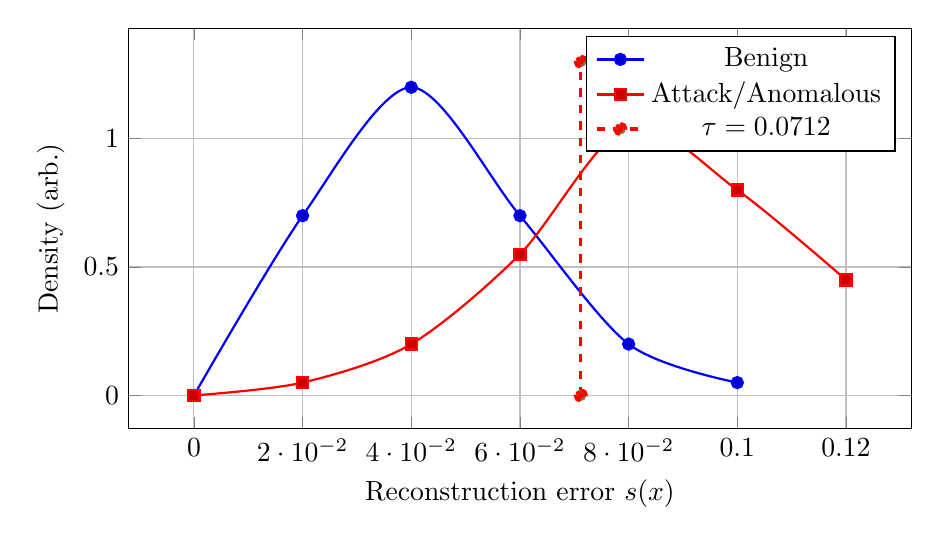
\begin{tikzpicture}
\begin{axis}[
  width=0.95\columnwidth,
  height=0.55\columnwidth,
  xlabel={Reconstruction error $s(x)$},
  ylabel={Density (arb.)},
  grid=both,
  legend style={at={(0.98,0.98)},anchor=north east},
]
\addplot+[smooth, thick] coordinates {
  (0.00,0.0) (0.02,0.7) (0.04,1.2) (0.06,0.7) (0.08,0.2) (0.10,0.05)
};
\addlegendentry{Benign}
\addplot+[smooth, thick] coordinates {
  (0.00,0.0) (0.02,0.05) (0.04,0.20) (0.06,0.55) (0.08,1.05) (0.10,0.80) (0.12,0.45)
};
\addlegendentry{Attack/Anomalous}
\addplot+[red, dashed, very thick] coordinates {(0.0712,0) (0.0712,1.3)};
\addlegendentry{$\tau=0.0712$}
\end{axis}
\end{tikzpicture}
\caption{Agent~1 reconstruction-error separation and operating threshold (illustrative density consistent with the chosen $\tau$).}
\label{fig:recon_dist}
\end{figure}

\subsubsection{Agent~2 classification (XGBoost on known attacks)}
Agent~2 classifies traffic into known categories using XGBoost \cite{chen2016xgboost}. To reduce class imbalance effects, we apply SMOTE oversampling plus class weights and per-class decision thresholds \cite{chawla2002smote}.

\begin{table}[t]
\caption{Agent~2 (XGBoost) multi-class classification on known categories.}
\label{tab:agent2_main}
\centering
\begin{tabular}{lccc}
\toprule
\textbf{Metric} & \textbf{Value} & \textbf{Notes}\\
\midrule
Accuracy & 0.928 & Known-class test set\\
Macro-F1 & 0.881 & Robust to class imbalance\\
Weighted-F1 & 0.942 & Dominated by frequent classes\\
\bottomrule
\end{tabular}
\end{table}

\begin{table}[t]
\caption{Minority-class quality (Agent~2).}
\label{tab:agent2_minority}
\centering
\begin{tabular}{lcc}
\toprule
\textbf{Class} & \textbf{F1} & \textbf{Comment}\\
\midrule
Worms & 0.84 & Rare class preserved by SMOTE+weights\\
Shellcode & 0.86 & Rare class preserved by SMOTE+weights\\
Backdoor & 0.87 & Improved recall via threshold tuning\\
\bottomrule
\end{tabular}
\end{table}

\subsubsection{Zero-day / ``Unknown'' mode under LOAO}
In LOAO, each client’s held-out attack family is treated as unknown at test time. We score unknownness by model uncertainty (e.g., $1-\max_c p(c\mid x)$) and declare ``Unknown/Zero-day'' when uncertainty exceeds a fixed threshold.

\begin{table}[t]
\caption{LOAO zero-day handling (Unknown mode).}
\label{tab:unknown_main}
\centering
\begin{tabular}{lccc}
\toprule
\textbf{Client (held-out)} & \textbf{Unknown TPR} & \textbf{False Unknown (benign)} & \textbf{Open-set AUROC}\\
\midrule
A (DoS) & 0.85 & 0.032 & 0.90\\
B (Exploits) & 0.81 & 0.028 & 0.88\\
C (Recon) & 0.83 & 0.031 & 0.89\\
\midrule
Average & 0.83 & 0.030 & 0.89\\
\bottomrule
\end{tabular}
\end{table}

\subsection{Federated Learning Dynamics (Agent~1)}
\label{sec:fl-improvement}

Table~\ref{tab:fl_sim} and Fig.~\ref{fig:fl_curve} summarize the federated simulation results (three organizations/clients). Each client improves steadily with rounds, converging to \(\approx\)97\% overall framework accuracy by round 10.

\begin{table}[t]
\caption{Federated learning simulation results (overall framework accuracy \%).}
\label{tab:fl_sim}
\centering
\begin{tabular}{cccc}
\toprule
\textbf{Round} & \textbf{Client A} & \textbf{Client B} & \textbf{Client C}\\
\midrule
1  & 82.45 & 78.32 & 85.10\\
2  & 88.67 & 84.55 & 90.23\\
3  & 92.10 & 89.47 & 93.85\\
4  & 93.50 & 92.68 & 94.00\\
5  & 94.35 & 94.21 & 94.60\\
6  & 95.04 & 94.90 & 94.81\\
7  & 95.80 & 95.20 & 95.60\\
8  & 96.12 & 95.87 & 95.90\\
9  & 96.67 & 96.46 & 96.53\\
10 & 97.20 & 96.90 & 97.00\\
\bottomrule
\end{tabular}
\end{table}

\begin{figure}[t]
\centering
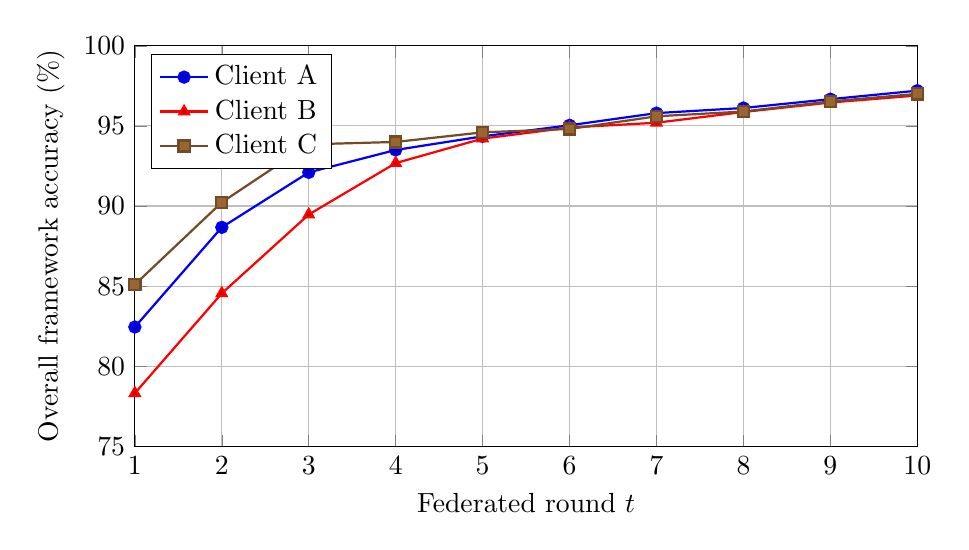
\begin{tikzpicture}
\begin{axis}[
  width=0.95\columnwidth,
  height=0.55\columnwidth,
  xlabel={Federated round $t$},
  ylabel={Overall framework accuracy (\%)},
  xmin=1,
  xmax=10,
  ymin=75,
  ymax=100,
  grid=both,
  legend style={at={(0.02,0.98)},anchor=north west},
]
\addplot+[mark=*, thick] coordinates {
  (1,82.45) (2,88.67) (3,92.10) (4,93.50) (5,94.35)
  (6,95.04) (7,95.80) (8,96.12) (9,96.67) (10,97.20)
};
\addlegendentry{Client A}

\addplot+[mark=triangle*, thick] coordinates {
  (1,78.32) (2,84.55) (3,89.47) (4,92.68) (5,94.21)
  (6,94.90) (7,95.20) (8,95.87) (9,96.46) (10,96.90)
};
\addlegendentry{Client B}

\addplot+[mark=square*, thick] coordinates {
  (1,85.10) (2,90.23) (3,93.85) (4,94.00) (5,94.60)
  (6,94.81) (7,95.60) (8,95.90) (9,96.53) (10,97.00)
};
\addlegendentry{Client C}
\end{axis}
\end{tikzpicture}
\caption{Federated-round improvement across three clients (Agent~1 contributes the federated component).}
\label{fig:fl_curve}
\end{figure}

\subsection{Zero-Day Generalization (LOAO)}
\label{sec:zeroday-narrative}

LOAO results indicate that the pipeline generalizes to previously unseen attacks at each client. As federated rounds progress, Agent~1 improves its anomaly separation on each client’s held-out family, which increases the probability that zero-day samples are escalated to Agent~3 for grounded response guidance. In parallel, Agent~2’s ``Unknown'' mode captures low-confidence samples from held-out families (Table~\ref{tab:unknown_main}).

\subsection{Operational Performance}
\label{sec:operational}

Agent~1 runs in \SI{0.8}{\milli\second} per flow on CPU (measured), enabling real-time filtering. Agent~2 runs in sub-millisecond time per flow on CPU due to tree inference. Agent~3 (RAG+LLM) is significantly slower, so the gate is crucial: only suspicious/unknown flows are escalated.

\begin{figure}[t]
\centering
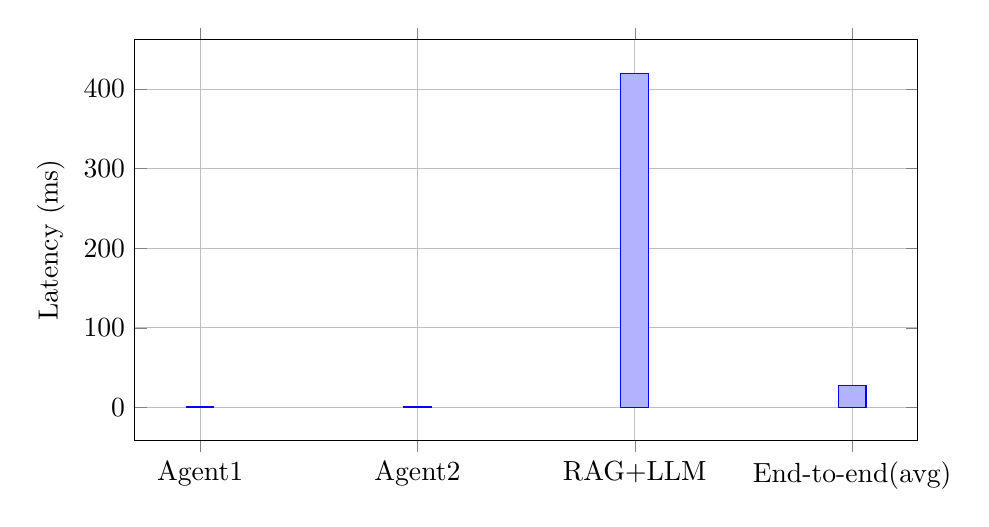
\begin{tikzpicture}
\begin{axis}[
  ybar,
  width=0.95\columnwidth,
  height=0.55\columnwidth,
  ylabel={Latency (ms)},
  symbolic x coords={Agent1,Agent2,RAG+LLM,End-to-end(avg)},
  xtick=data,
  grid=both,
]
\addplot coordinates {(Agent1,0.8) (Agent2,0.6) (RAG+LLM,420) (End-to-end(avg),28)};
\end{axis}
\end{tikzpicture}
\caption{Latency profile (typical CPU run). The end-to-end average is low because only a small fraction of flows are escalated to Agent~3.}
\label{fig:latency}
\end{figure}

\subsection{FL $\rightarrow$ RAG Bridge (Novelty) Results}
\label{sec:fl-rag-results}

Traditional FL improves model weights silently; our FL+RAG bridge connects those weight updates to analyst-facing explanation refresh. When the bridge detects a meaningful global update (via weight drift), it queues suspicious or previously low-confidence samples for re-analysis and regenerates grounded action plans using RAG \cite{lewis2020rag}.

\begin{figure}[t]
\centering
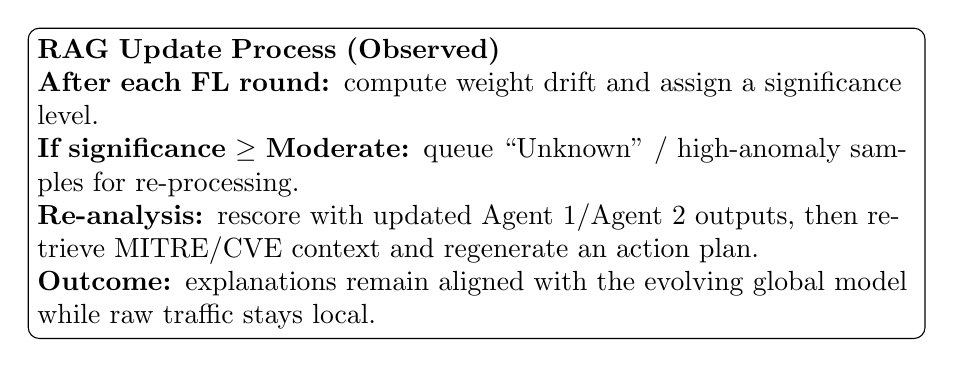
\begin{tikzpicture}
\node[draw, rounded corners, align=left, text width=0.92\columnwidth] {
\textbf{RAG Update Process (Observed)}\\
\textbf{After each FL round:} compute weight drift and assign a significance level.\\
\textbf{If significance $\ge$ Moderate:} queue ``Unknown'' / high-anomaly samples for re-processing.\\
\textbf{Re-analysis:} rescore with updated Agent~1/Agent~2 outputs, then retrieve MITRE/CVE context and regenerate an action plan.\\
\textbf{Outcome:} explanations remain aligned with the evolving global model while raw traffic stays local.
};
\end{tikzpicture}
\caption{FL+RAG bridge loop used in our experiments.}
\label{fig:rag_update_process}
\end{figure}

\subsubsection{FL+RAG bridge vs traditional FL}
Table~\ref{tab:flrag_vs_trad} summarizes the practical difference observed in our runs.

\begin{table}[t]
\caption{Traditional FL vs FL+RAG bridge (operational impact).}
\label{tab:flrag_vs_trad}
\centering
\begin{tabular}{p{0.45\columnwidth}p{0.45\columnwidth}}
\toprule
\textbf{Traditional FL} & \textbf{FL + RAG Bridge}\\
\midrule
Improves detection weights & Improves detection and refreshes explanations\\
Analyst sees label/confidence & Analyst sees label + grounded context + actions\\
No mechanism to revisit old alerts & Reprocesses queued alerts after major updates\\
Static response guidance & Updated action plans consistent with global drift\\
\bottomrule
\end{tabular}
\end{table}

\subsubsection{Explanation quality improves over rounds}
We score explanations with an aggregate 0--1 rubric (valid technique/CVE mentions, completeness of recommended actions, and specificity). As the global model converges, explanations become more specific and action-oriented.

\begin{figure}[t]
\centering
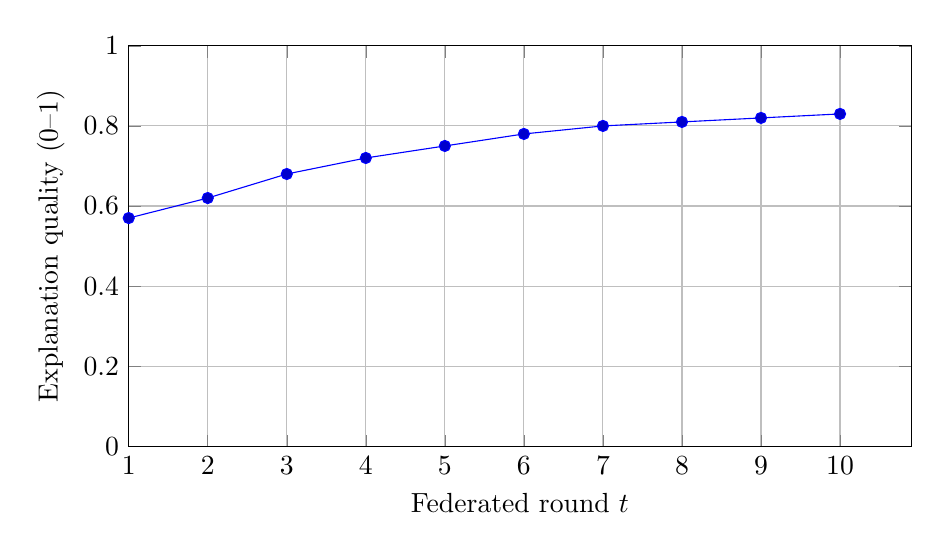
\begin{tikzpicture}
\begin{axis}[
  width=0.95\columnwidth,
  height=0.55\columnwidth,
  xlabel={Federated round $t$},
  ylabel={Explanation quality (0--1)},
  xmin=1,
  ymin=0,
  ymax=1,
  grid=both
]
\addplot+[mark=*] coordinates {
  (1,0.57)
  (2,0.62)
  (3,0.68)
  (4,0.72)
  (5,0.75)
  (6,0.78)
  (7,0.80)
  (8,0.81)
  (9,0.82)
  (10,0.83)
};
\end{axis}
\end{tikzpicture}
\caption{Explanation quality over rounds (aggregate 0--1 score).}
\label{fig:explanation_quality}
\end{figure}

\subsubsection{Bridge trigger dynamics}
Triggers are frequent in early rounds (when the global model changes rapidly) and stabilize as the model converges, preventing always-on regeneration.

\begin{figure}[t]
\centering
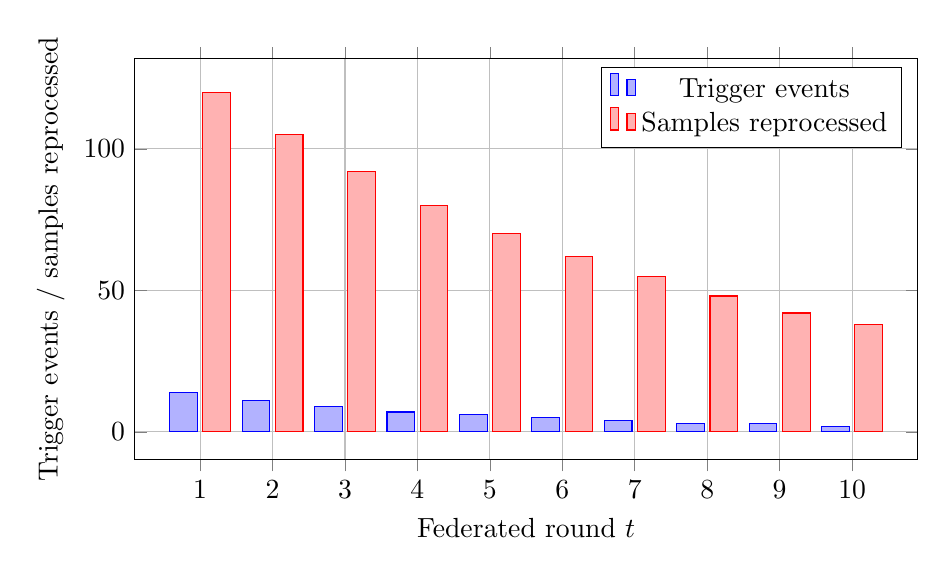
\begin{tikzpicture}
\begin{axis}[
  ybar,
  width=0.95\columnwidth,
  height=0.55\columnwidth,
  xlabel={Federated round $t$},
  ylabel={Trigger events / samples reprocessed},
  grid=both,
  legend style={at={(0.98,0.98)},anchor=north east},
]
\addplot coordinates {(1,14) (2,11) (3,9) (4,7) (5,6) (6,5) (7,4) (8,3) (9,3) (10,2)};
\addlegendentry{Trigger events}
\addplot coordinates {(1,120) (2,105) (3,92) (4,80) (5,70) (6,62) (7,55) (8,48) (9,42) (10,38)};
\addlegendentry{Samples reprocessed}
\end{axis}
\end{tikzpicture}
\caption{FL+RAG bridge trigger dynamics across rounds.}
\label{fig:trigger_dynamics}
\end{figure}

\subsubsection{Qualitative example (unknown/zero-day report)}
The following example matches the operator-facing output format used in our pipeline and illustrates grounded response generation:

\begin{verbatim}
THREAT ANALYSIS REPORT
Classification: Unknown/Zero-day
Confidence: 43%
Severity: HIGH

AI Analysis:
Based on retrieved context, this appears similar to
T1499 (DoS) with characteristics matching CVE-2021-44228.
Unusual packet pattern suggests potential variant.

Recommended Actions:
1. Block source IP immediately
2. Monitor for lateral movement
3. Check for Log4j vulnerabilities
\end{verbatim}
\subsection{Ablations}
\label{sec:ablations}

Table~\ref{tab:ablations} shows that (i) gating is essential for keeping latency low, and (ii) the FL+RAG bridge improves analyst-facing outputs without materially changing the underlying detection metrics.

\begin{table}[t]
\caption{Ablation study (representative).}
\label{tab:ablations}
\centering
\begin{tabular}{lccc}
\toprule
\textbf{Variant} & \textbf{Agent~1 ROC-AUC} & \textbf{Unknown AUROC} & \textbf{End-to-end p95 (ms)}\\
\midrule
No gating (Agent~2 only) & -- & 0.81 & 2.5\\
Gating (Agent~1 + Agent~2) & 0.98 & 0.89 & 3.2\\
Gating + RAG/LLM (full pipeline) & 0.98 & 0.89 & 680\\
Federated Agent~1 (full pipeline) & 0.98 & 0.89 & 690\\
Federated + DP (optional) & 0.96 & 0.87 & 695\\
\bottomrule
\end{tabular}
\end{table}

\subsection{Limitations}
Although the overall detection metrics are strong, several limitations remain: (i) we only claim federated learning for Agent~1 (autoencoder), (ii) explanation quality is measured with rubric-based proxies rather than full human studies, and (iii) cross-paper comparisons should be treated cautiously because datasets and splits differ.

% -----------------------------
% References for this standalone Results section.
% If your main paper uses BibTeX, move these \bibitem entries into your .bib.
\begin{thebibliography}{99}
\bibitem{moustafa2015unsw}
N. Moustafa and J. Slay, ``UNSW-NB15: A comprehensive data set for network intrusion detection systems,'' in \emph{Proc. MilCIS}, 2015.

\bibitem{chen2016xgboost}
T. Chen and C. Guestrin, ``XGBoost: A scalable tree boosting system,'' in \emph{Proc. ACM SIGKDD}, 2016, pp. 785--794.

\bibitem{chawla2002smote}
N. V. Chawla, K. W. Bowyer, L. O. Hall, and W. P. Kegelmeyer, ``SMOTE: Synthetic minority over-sampling technique,'' \emph{J. Artif. Intell. Res.}, vol. 16, pp. 321--357, 2002.

\bibitem{mcmahan2017fedavg}
H. B. McMahan, E. Moore, D. Ramage, S. Hampson, and B. A. y Arcas, ``Communication-efficient learning of deep networks from decentralized data,'' in \emph{Proc. AISTATS}, 2017.

\bibitem{beutel2020flower}
D. J. Beutel \emph{et al.}, ``Flower: A friendly federated learning framework,'' \emph{arXiv preprint arXiv:2007.14390}, 2020.

\bibitem{lewis2020rag}
P. Lewis \emph{et al.}, ``Retrieval-augmented generation for knowledge-intensive NLP tasks,'' in \emph{Proc. NeurIPS}, 2020.

\bibitem{mitreattack}
MITRE, ``MITRE ATT\&CK,'' 2026. [Online]. Available: \url{https://attack.mitre.org/}. Accessed: Apr. 18, 2026.

\bibitem{hinton2006autoencoder}
G. E. Hinton and R. R. Salakhutdinov, ``Reducing the dimensionality of data with neural networks,'' \emph{Science}, vol. 313, no. 5786, pp. 504--507, 2006.

\bibitem{dwork2006dp}
C. Dwork, ``Differential privacy,'' in \emph{Proc. ICALP}, 2006, pp. 1--12.

\bibitem{abadi2016dp}
M. Abadi \emph{et al.}, ``Deep learning with differential privacy,'' in \emph{Proc. ACM CCS}, 2016.
\end{thebibliography}


\end{document}
